
\section{\ref{PS:Q:Performance}}

\textit{Can we create a solution that scales such that the number of turbines does not impact the regulation cycle time?}

\subsection{Experiments}
\label{sec:Exper:perfom}

%Scalability is by Bondi\cite{Bondi:2000:CSI:350391.350432} defined as \textit{the systems ability to accommodate an increasing number of elements or objects, to process growing volumes of work gracefully, and/or to be susceptible to enlargement}.

The \ref{PS:Q:Performance} question asks if the proposed decentralized solution is able to keep a constant regulation cycle time independent from the number of turbines. This problem operates in a 3-dimensional space with regulation cycle time (ms), number of cache reads and number of turbines as parameters. To study the correlation between the parameters, we isolate two parameters by making the third constant.

Thus to fully address \ref{PS:Q:Performance} this experiment has been divided into two experiments:
 
\begin{description}
	\item[Experiment 1] aims to investigate the anti-correlation between the implemented sleep time of the regulation cycle and the number of cache reads for the decentralized system. This is relevant because changing the sleep time is expected to impact the number of cache reads, since an increase in sleep time increases the time Connext has to overwrite received states, thus decreasing the number of cache reads (as explained in \cref{sec:cachereads}: Cache reads). Thus the constant for this is experiment is the number of turbines.
	\item[Experiment 2] aims to investigate the impact on the regulation cycle time and the number of cache reads when increasing the number of turbines in the decentralized solution, and thus answer the \ref{PS:Q:Performance} problem. The constant for this experiment is the sleep time.
\end{description}

The cycle regulation time of the decentralized solution is defined as the difference between the receive timestamp of the oldest turbine state(tOldestState) received and the timestamp sampled right after, a new turbine state has been sent (tSent) (as illustrated on \cref{fig:timingDecentral}):

$$regulation~cycle~time=tSent-tOldestState$$

\begin{figure}[b]
	

{ %The brackets issolate the enviroment

\makeatletter
\ifcsname c@wavenum\endcsname %Only create one counter
\else
	\newcounter{wavenum}
\fi
\makeatother

\newcommand*{\bitvector}[3]{
  \draw[fill=#3] (t_cur) -- ++( .1, .3) -- ++(#2-.2,0) -- ++(.1, -.3)
                         -- ++(-.1,-.3) -- ++(.2-#2,0) -- cycle;
  \path (t_cur) -- node[anchor=mid](textNode) {#1} ++(#2,0) node[time] (t_cur) {};
}

% \known{val}{length}
\newcommand*{\known}[2]{
    \bitvector{#1}{#2}{white}
}

% \unknown{length}
\newcommand*{\unknown}[2]{
    \bitvector{#1}{#2}{black!20}
}

% \nextwave{name}
\newcommand{\nextwave}[1]{
  %\path (0,\value{wavenum}) node[left] {#1} node[time] (t_cur) {};
  \path (0,\value{wavenum}) node[time] (t_cur) {};
  \addtocounter{wavenum}{-1}
}

%\newcommand{\timeSpanLabel}{
%	\node (CycleTimeLabel) [rectangle, above = 0.25cm of textNode, inner sep=10pt] {CycleTime};	  
%}

\newcommand{\timeSpanLabel}{
	\node (CycleTimeLabel) [rectangle, above = 1.02cm of t_cur, inner sep=0pt] {Regulation cycle time};
}

\newcommand{\timeSpanA}{
	\node (t_timeSpanA) [point, above = 0 of t_cur] {};	  
}

\newcommand{\timeSpanB}{
	\node (t_timeSpanB) [point, above =0 of t_cur] {};
	
	\graph[use existing nodes]{
		t_timeSpanA --[time span=1cm] CycleTimeLabel;
		CycleTimeLabel.south --[time span=-0.24cm] t_timeSpanB;
	}; 
	
}

%%% End of timing.sty

\begin{tikzpicture}[
	point/.style={inner sep=0pt}, %circle,minimum size=2pt,fill=red},
	draw=black, 
	yscale=.8,
	xscale=1,
	hv path/.style={to path={-| (\tikztotarget)}},
	vh path/.style={to path={|- (\tikztotarget)}},
	skip loop v/.style={to path={-- ++(#1,0) |- (\tikztotarget)}},		
	skip loop h/.style={to path={-- ++(0,#1) -| (\tikztotarget)}},
	time span/.style={to path={-- ++(0,#1) -| (\tikztotarget)}},
	graphs/every graph/.style={edges=rounded corners}	
]
	
\tikzstyle{time}=[coordinate]
\setlength{\unitlength}{1cm}
\setcounter{wavenum}{0}

	\nextwave{} \timeSpanA \unknown{readStates}{3} \unknown{calculate}{3} \timeSpanLabel \unknown{setSetpoint}{3} \unknown{sendState}{3} \timeSpanB \known{wait}{2}
	\nextwave{} \known{reciveStates}{14}
\end{tikzpicture}
}

	\caption{Decentralized regulation time}
	\label{fig:timingDecentral}
\end{figure}

The timestamp of the oldest turbine state is used to include network traffic in the regulation cycle time, as opposed to just sampling the time locally. Note that by this definition, it is possible for regulation cycle time to be lower than the sleep time, even though the sleep operation is a part of the regulation cycle. 


\subsection{Experiment 1: How sleep time impacts the regulation cycle time and the number of cache reads}
\label{subsec:Exper:perfom:1}
The purpose of this experiment is to show how the sleep time affects the number of cache reads and the regulation cycle time for the decentralized solution (see \cref{sec:cachereads} for cache reads description).  
The experiment is performed with cycle time t=\testCycletimeNumbers.  

The following procedure is used each time the experiment is performed:
\begin{enumerate}
	\item Start the system with a cycle time of t ms and 50 turbines.
	\item Make sure the system is stable.
	\item Start logging the regulation cycle time and the number of cache reads.
	\item Stop logging after 50 seconds.
\end{enumerate}

50 seconds of logging provided 59000 data samples as the lowest amount of data samples for a single data set (the data set using 50 ms sleep time). Thus each data set of this experiment has been plotted using 59000 data samples.

\subsection{Experiment 2: How the number of turbines impacts the regulation cycle time and the number of cache reads}
\label{subsec:Exper:perfom:2}
The purpose of this experiment is to answer the \ref{PS:Q:Performance} problem, by showing how the number of turbines affects the regulation cycle time for the decentralized solution. To complete the picture we also investigate how the number of turbines affects the cache reads, since an expected side effect of increasing the number of turbines also increases the number of cache reads as described in \cref{sec:cachereads}.

The experiments are performed with n=\testTurbineNumbers ~turbines. The sleep time is set to 20 ms and is constant for this experiment.

The test system is expected to be running only one instance in a real life implementation, therefore the machine logging the data will only run one instance and the supporting machines will run the rest generating system load.

The following procedure is used each time the experiment is performed:
\begin{enumerate}
	\item Start the system with n turbines.
	\item Make sure the system is stable.
	\item Start logging the reported regulation run time and the number of cache reads.
	\item Stop logging after 50 seconds.
\end{enumerate}

50 seconds of logging provided 14500 data samples as the lowest amount of data samples for a single data set (the data using 5 turbines). Thus each data set of this experiment has been plotted using 14500 data samples.

\subsection{Results} \label{sec:exp:performance}

We use the following box plot type (for \cref{fig:exp:decen:sleep} and \cref{fig:exp:decen:turbines}): The central mark is the median, the edges of the box are the 25th and 75th percentiles, the whiskers extend to the most extreme data points not considered outliers, and outliers are plotted individually. The whisker length is denoted as 1.5 IQR. 

\subsubsection{\nameref{subsec:Exper:perfom:1}}

\begin{figure}[h!]
	\centering
%	\begin{tikzpicture}
\begin{axis}
[
width=\resultsFigureWidthScale\textwidth,
axis y line*=left,
xlabel=Sleeptime (ms),
ylabel=Regulation cycle time (ms),
ymin = 0,
xtick={1, 2, 3, 4, 5, 6, 7, 8, 9},
xticklabels={10, 15, 20, 25, 30, 35, 40, 45, 50},
boxplot/draw direction=y
]

%% /home/stefan/work/TestResults/Test6_Decentralized_12-7-2014_1327/nCycleTime/DecentralizedLog1.csv
\buildBoxPlot{10.578002}{15.286001}{9.942}{148.911}{0.415002}

%% /home/stefan/work/TestResults/Test6_Decentralized_12-7-2014_1327/nCycleTime/DecentralizedLog2.csv
\buildBoxPlot{15.026002}{15.383002}{14.312002}{26.729001}{1.379}

%% /home/stefan/work/TestResults/Test6_Decentralized_12-7-2014_1327/nCycleTime/DecentralizedLog3.csv
\buildBoxPlot{19.926}{20.380001}{18.979001}{29.932002}{0.435}

%% /home/stefan/work/TestResults/Test6_Decentralized_12-7-2014_1327/nCycleTime/DecentralizedLog4.csv
\buildBoxPlot{25.079001}{25.322}{24.637001}{32.794001}{12.225002}

%% /home/stefan/work/TestResults/Test6_Decentralized_12-7-2014_1327/nCycleTime/DecentralizedLog5.csv
\buildBoxPlot{30.099}{30.363}{29.565001}{42.436}{4.466}

%% /home/stefan/work/TestResults/Test6_Decentralized_12-7-2014_1327/nCycleTime/DecentralizedLog6.csv
\buildBoxPlot{35.153001}{35.328002}{34.853001}{45.836001}{10.347}

%% /home/stefan/work/TestResults/Test6_Decentralized_12-7-2014_1327/nCycleTime/DecentralizedLog7.csv
\buildBoxPlot{40.157001}{40.434001}{39.626}{58.338001}{6.398001}

%% /home/stefan/work/TestResults/Test6_Decentralized_12-7-2014_1327/nCycleTime/DecentralizedLog8.csv
\buildBoxPlot{45.185}{45.330001}{44.928002}{50.089}{29.313}

%% /home/stefan/work/TestResults/Test6_Decentralized_12-7-2014_1327/nCycleTime/DecentralizedLog9.csv
\buildBoxPlot{49.958002}{50.391001}{49.019}{64.611002}{4.846}


\addplot[thick, red!70] coordinates {
	(1 ,10.578002)
	(2 ,15.026002)
	(3 ,19.926)
	(4 ,25.079001)
	(5 ,30.099)
	(6 ,35.153001)
	(7 ,40.157001)
	(8 ,45.185)
	(9 ,49.958002)
	
};

\end{axis}
\end{tikzpicture}

	% This file was created by matlab2tikz.
% Minimal pgfplots version: 1.3
%
%The latest updates can be retrieved from
%  http://www.mathworks.com/matlabcentral/fileexchange/22022-matlab2tikz
%where you can also make suggestions and rate matlab2tikz.
%
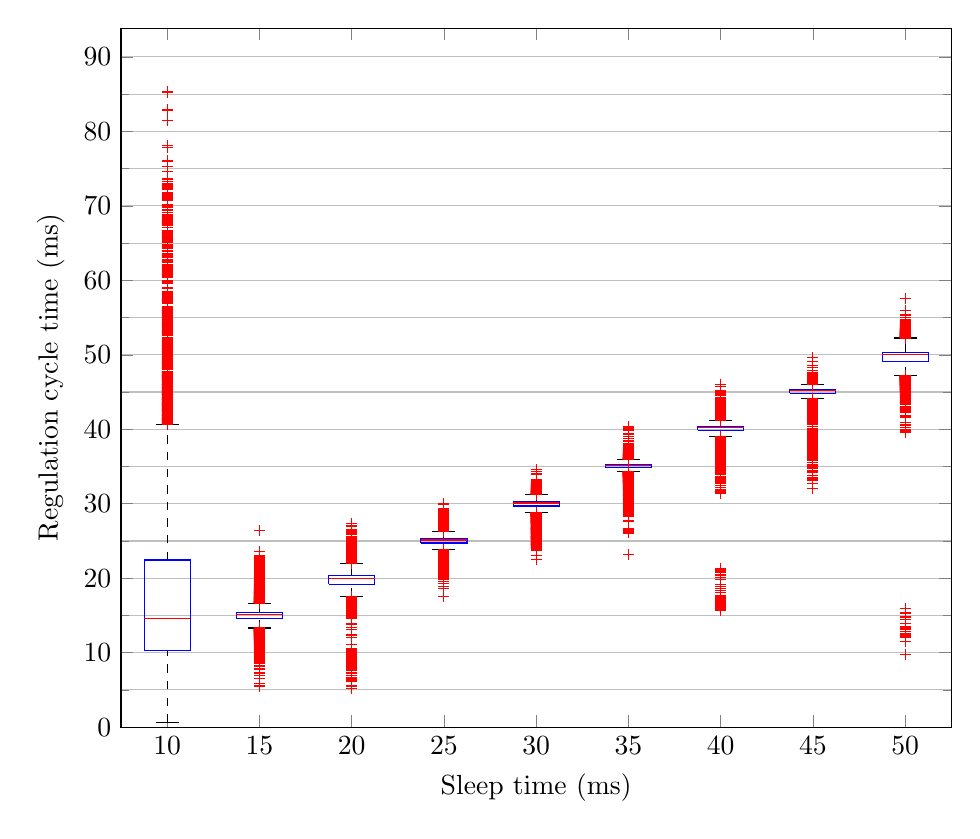
\begin{tikzpicture}

\begin{axis}[%
	width=\resultsPlotWidthScale\textwidth,
	xmin=0.5,
	xmax=9.5,
	ymin=0,
	xlabel=Sleep time (ms),
	ylabel=Regulation cycle time (ms),
	xtick={1, 2, 3, 4, 5, 6, 7, 8, 9},
	xticklabels={10, 15, 20, 25, 30, 35, 40, 45, 50},
	ymajorgrids=true,
	yminorgrids=true,
	minor y tick num=1
]
\addplot [color=black,dashed,forget plot]
  table[row sep=crcr]{%
1 22.4525015\\
1 40.601\\
};
\addplot [color=black,dashed,forget plot]
  table[row sep=crcr]{%
2 15.386001\\
2 16.628001\\
};
\addplot [color=black,dashed,forget plot]
  table[row sep=crcr]{%
3 20.328002\\
3 21.995001\\
};
\addplot [color=black,dashed,forget plot]
  table[row sep=crcr]{%
4 25.350001\\
4 26.279001\\
};
\addplot [color=black,dashed,forget plot]
  table[row sep=crcr]{%
5 30.312001\\
5 31.219001\\
};
\addplot [color=black,dashed,forget plot]
  table[row sep=crcr]{%
6 35.315001\\
6 35.919001\\
};
\addplot [color=black,dashed,forget plot]
  table[row sep=crcr]{%
7 40.380501\\
7 41.197\\
};
\addplot [color=black,dashed,forget plot]
  table[row sep=crcr]{%
8 45.316001\\
8 46.006001\\
};
\addplot [color=black,dashed,forget plot]
  table[row sep=crcr]{%
9 50.356\\
9 52.254001\\
};
\addplot [color=black,dashed,forget plot]
  table[row sep=crcr]{%
1 0.623001\\
1 10.3525005\\
};
\addplot [color=black,dashed,forget plot]
  table[row sep=crcr]{%
2 13.316001\\
2 14.558\\
};
\addplot [color=black,dashed,forget plot]
  table[row sep=crcr]{%
3 17.548001\\
3 19.215501\\
};
\addplot [color=black,dashed,forget plot]
  table[row sep=crcr]{%
4 23.8\\
4 24.73\\
};
\addplot [color=black,dashed,forget plot]
  table[row sep=crcr]{%
5 28.793002\\
5 29.704001\\
};
\addplot [color=black,dashed,forget plot]
  table[row sep=crcr]{%
6 34.306001\\
6 34.9110015\\
};
\addplot [color=black,dashed,forget plot]
  table[row sep=crcr]{%
7 39.023\\
7 39.836\\
};
\addplot [color=black,dashed,forget plot]
  table[row sep=crcr]{%
8 44.166001\\
8 44.855501\\
};
\addplot [color=black,dashed,forget plot]
  table[row sep=crcr]{%
9 47.193001\\
9 49.09\\
};
\addplot [color=black,solid,forget plot]
  table[row sep=crcr]{%
0.875 40.601\\
1.125 40.601\\
};
\addplot [color=black,solid,forget plot]
  table[row sep=crcr]{%
1.875 16.628001\\
2.125 16.628001\\
};
\addplot [color=black,solid,forget plot]
  table[row sep=crcr]{%
2.875 21.995001\\
3.125 21.995001\\
};
\addplot [color=black,solid,forget plot]
  table[row sep=crcr]{%
3.875 26.279001\\
4.125 26.279001\\
};
\addplot [color=black,solid,forget plot]
  table[row sep=crcr]{%
4.875 31.219001\\
5.125 31.219001\\
};
\addplot [color=black,solid,forget plot]
  table[row sep=crcr]{%
5.875 35.919001\\
6.125 35.919001\\
};
\addplot [color=black,solid,forget plot]
  table[row sep=crcr]{%
6.875 41.197\\
7.125 41.197\\
};
\addplot [color=black,solid,forget plot]
  table[row sep=crcr]{%
7.875 46.006001\\
8.125 46.006001\\
};
\addplot [color=black,solid,forget plot]
  table[row sep=crcr]{%
8.875 52.254001\\
9.125 52.254001\\
};
\addplot [color=black,solid,forget plot]
  table[row sep=crcr]{%
0.875 0.623001\\
1.125 0.623001\\
};
\addplot [color=black,solid,forget plot]
  table[row sep=crcr]{%
1.875 13.316001\\
2.125 13.316001\\
};
\addplot [color=black,solid,forget plot]
  table[row sep=crcr]{%
2.875 17.548001\\
3.125 17.548001\\
};
\addplot [color=black,solid,forget plot]
  table[row sep=crcr]{%
3.875 23.8\\
4.125 23.8\\
};
\addplot [color=black,solid,forget plot]
  table[row sep=crcr]{%
4.875 28.793002\\
5.125 28.793002\\
};
\addplot [color=black,solid,forget plot]
  table[row sep=crcr]{%
5.875 34.306001\\
6.125 34.306001\\
};
\addplot [color=black,solid,forget plot]
  table[row sep=crcr]{%
6.875 39.023\\
7.125 39.023\\
};
\addplot [color=black,solid,forget plot]
  table[row sep=crcr]{%
7.875 44.166001\\
8.125 44.166001\\
};
\addplot [color=black,solid,forget plot]
  table[row sep=crcr]{%
8.875 47.193001\\
9.125 47.193001\\
};
\addplot [color=blue,solid,forget plot]
  table[row sep=crcr]{%
0.75  10.3525005\\
0.75  22.4525015\\
1.25  22.4525015\\
1.25  10.3525005\\
0.75  10.3525005\\
};
\addplot [color=blue,solid,forget plot]
  table[row sep=crcr]{%
1.75  14.558\\
1.75  15.386001\\
2.25  15.386001\\
2.25  14.558\\
1.75  14.558\\
};
\addplot [color=blue,solid,forget plot]
  table[row sep=crcr]{%
2.75  19.215501\\
2.75  20.328002\\
3.25  20.328002\\
3.25  19.215501\\
2.75  19.215501\\
};
\addplot [color=blue,solid,forget plot]
  table[row sep=crcr]{%
3.75  24.73\\
3.75  25.350001\\
4.25  25.350001\\
4.25  24.73\\
3.75  24.73\\
};
\addplot [color=blue,solid,forget plot]
  table[row sep=crcr]{%
4.75  29.704001\\
4.75  30.312001\\
5.25  30.312001\\
5.25  29.704001\\
4.75  29.704001\\
};
\addplot [color=blue,solid,forget plot]
  table[row sep=crcr]{%
5.75  34.9110015\\
5.75  35.315001\\
6.25  35.315001\\
6.25  34.9110015\\
5.75  34.9110015\\
};
\addplot [color=blue,solid,forget plot]
  table[row sep=crcr]{%
6.75  39.836\\
6.75  40.380501\\
7.25  40.380501\\
7.25  39.836\\
6.75  39.836\\
};
\addplot [color=blue,solid,forget plot]
  table[row sep=crcr]{%
7.75  44.855501\\
7.75  45.316001\\
8.25  45.316001\\
8.25  44.855501\\
7.75  44.855501\\
};
\addplot [color=blue,solid,forget plot]
  table[row sep=crcr]{%
8.75  49.09\\
8.75  50.356\\
9.25  50.356\\
9.25  49.09\\
8.75  49.09\\
};
\addplot [color=red,solid,forget plot]
  table[row sep=crcr]{%
0.75  14.547501\\
1.25  14.547501\\
};
\addplot [color=red,solid,forget plot]
  table[row sep=crcr]{%
1.75  15.084002\\
2.25  15.084002\\
};
\addplot [color=red,solid,forget plot]
  table[row sep=crcr]{%
2.75  19.9260015\\
3.25  19.9260015\\
};
\addplot [color=red,solid,forget plot]
  table[row sep=crcr]{%
3.75  25.133\\
4.25  25.133\\
};
\addplot [color=red,solid,forget plot]
  table[row sep=crcr]{%
4.75  30.104501\\
5.25  30.104501\\
};
\addplot [color=red,solid,forget plot]
  table[row sep=crcr]{%
5.75  35.1650005\\
6.25  35.1650005\\
};
\addplot [color=red,solid,forget plot]
  table[row sep=crcr]{%
6.75  40.182001\\
7.25  40.182001\\
};
\addplot [color=red,solid,forget plot]
  table[row sep=crcr]{%
7.75  45.1500005\\
8.25  45.1500005\\
};
\addplot [color=red,solid,forget plot]
  table[row sep=crcr]{%
8.75  49.991\\
9.25  49.991\\
};
\addplot [color=blue,only marks,mark=+,mark options={solid,draw=red},forget plot]
  table[row sep=crcr]{%
1 40.603001\\
1 40.640001\\
1 40.642001\\
1 40.677001\\
1 40.685001\\
1 40.691001\\
1 40.698\\
1 40.701\\
1 40.731\\
1 40.74\\
1 40.770002\\
1 40.789\\
1 40.792\\
1 40.796\\
1 40.804001\\
1 40.946001\\
1 40.959001\\
1 40.960001\\
1 40.995002\\
1 41.007\\
1 41.061001\\
1 41.067\\
1 41.119\\
1 41.123\\
1 41.144001\\
1 41.152001\\
1 41.159\\
1 41.179\\
1 41.2\\
1 41.206\\
1 41.211001\\
1 41.226001\\
1 41.237\\
1 41.24\\
1 41.255001\\
1 41.299001\\
1 41.303001\\
1 41.362001\\
1 41.376\\
1 41.383001\\
1 41.400001\\
1 41.440001\\
1 41.443\\
1 41.446\\
1 41.477\\
1 41.489001\\
1 41.508\\
1 41.534001\\
1 41.559001\\
1 41.563001\\
1 41.621001\\
1 41.63\\
1 41.658\\
1 41.67\\
1 41.675\\
1 41.726\\
1 41.748\\
1 41.759\\
1 41.791\\
1 41.806\\
1 41.821001\\
1 41.824\\
1 41.842\\
1 41.858\\
1 41.86\\
1 41.863001\\
1 41.873001\\
1 41.922001\\
1 41.928\\
1 41.945001\\
1 41.972\\
1 41.995001\\
1 42.004\\
1 42.047\\
1 42.096\\
1 42.248\\
1 42.265001\\
1 42.274001\\
1 42.301\\
1 42.326\\
1 42.349001\\
1 42.349001\\
1 42.381001\\
1 42.403\\
1 42.451\\
1 42.453001\\
1 42.494\\
1 42.513001\\
1 42.521\\
1 42.526001\\
1 42.534\\
1 42.551001\\
1 42.574\\
1 42.599001\\
1 42.636001\\
1 42.651\\
1 42.652001\\
1 42.659\\
1 42.714\\
1 42.720001\\
1 42.734001\\
1 42.749\\
1 42.774\\
1 42.801001\\
1 42.819001\\
1 42.833001\\
1 42.868001\\
1 42.911\\
1 42.945\\
1 42.98\\
1 42.980001\\
1 42.996001\\
1 43.020001\\
1 43.042001\\
1 43.111\\
1 43.128001\\
1 43.131\\
1 43.139\\
1 43.141001\\
1 43.153002\\
1 43.175001\\
1 43.185001\\
1 43.225002\\
1 43.246\\
1 43.263001\\
1 43.279\\
1 43.320001\\
1 43.334\\
1 43.340001\\
1 43.349001\\
1 43.379001\\
1 43.381001\\
1 43.386001\\
1 43.392\\
1 43.392\\
1 43.405002\\
1 43.406\\
1 43.407001\\
1 43.454002\\
1 43.482\\
1 43.490001\\
1 43.492001\\
1 43.508\\
1 43.567001\\
1 43.585\\
1 43.609001\\
1 43.657\\
1 43.695\\
1 43.707001\\
1 43.71\\
1 43.746\\
1 43.815\\
1 43.819\\
1 43.825002\\
1 43.963\\
1 43.964\\
1 43.984002\\
1 43.986001\\
1 44.021002\\
1 44.025\\
1 44.027\\
1 44.055001\\
1 44.083001\\
1 44.109001\\
1 44.110001\\
1 44.117001\\
1 44.144001\\
1 44.159001\\
1 44.222001\\
1 44.294002\\
1 44.321001\\
1 44.384001\\
1 44.395\\
1 44.448\\
1 44.540001\\
1 44.594001\\
1 44.597001\\
1 44.607\\
1 44.625001\\
1 44.681001\\
1 44.682\\
1 44.696\\
1 44.696001\\
1 44.706001\\
1 44.708\\
1 44.711\\
1 44.739001\\
1 44.742001\\
1 44.746\\
1 44.781001\\
1 44.784\\
1 44.804\\
1 44.813001\\
1 44.822\\
1 44.837002\\
1 44.877001\\
1 44.919\\
1 44.932001\\
1 44.933001\\
1 44.947001\\
1 44.981001\\
1 45.005001\\
1 45.061001\\
1 45.086001\\
1 45.111001\\
1 45.111001\\
1 45.121001\\
1 45.171001\\
1 45.189001\\
1 45.206\\
1 45.241001\\
1 45.263001\\
1 45.266\\
1 45.288\\
1 45.349001\\
1 45.355001\\
1 45.365\\
1 45.448\\
1 45.485001\\
1 45.535\\
1 45.571\\
1 45.618\\
1 45.619001\\
1 45.630002\\
1 45.646001\\
1 45.658001\\
1 45.712001\\
1 45.762001\\
1 45.771001\\
1 45.876001\\
1 45.89\\
1 45.925001\\
1 45.939\\
1 45.963\\
1 45.963001\\
1 45.973001\\
1 46.003\\
1 46.009001\\
1 46.021001\\
1 46.032\\
1 46.041002\\
1 46.091001\\
1 46.110001\\
1 46.165001\\
1 46.197001\\
1 46.248001\\
1 46.319001\\
1 46.341001\\
1 46.366\\
1 46.41\\
1 46.475001\\
1 46.491001\\
1 46.496001\\
1 46.539\\
1 46.647001\\
1 46.650001\\
1 46.653001\\
1 46.687001\\
1 46.706\\
1 46.723001\\
1 46.763001\\
1 46.808\\
1 46.84\\
1 46.869\\
1 46.925\\
1 46.937\\
1 46.992001\\
1 46.998\\
1 47.004\\
1 47.011001\\
1 47.043\\
1 47.079002\\
1 47.131\\
1 47.14\\
1 47.142001\\
1 47.149\\
1 47.160001\\
1 47.169001\\
1 47.184001\\
1 47.189\\
1 47.194001\\
1 47.23\\
1 47.231001\\
1 47.276001\\
1 47.287001\\
1 47.345001\\
1 47.350001\\
1 47.377001\\
1 47.439001\\
1 47.459001\\
1 47.473001\\
1 47.559001\\
1 47.585\\
1 47.599002\\
1 47.612002\\
1 47.632\\
1 47.652001\\
1 47.697001\\
1 47.725\\
1 47.757001\\
1 47.777002\\
1 47.791001\\
1 47.975001\\
1 47.995\\
1 48.123002\\
1 48.127001\\
1 48.167001\\
1 48.187001\\
1 48.205001\\
1 48.239\\
1 48.256001\\
1 48.259\\
1 48.339001\\
1 48.349001\\
1 48.400001\\
1 48.466\\
1 48.543\\
1 48.556002\\
1 48.577\\
1 48.662001\\
1 48.739\\
1 48.739001\\
1 48.753001\\
1 48.766\\
1 48.832001\\
1 48.832001\\
1 48.858\\
1 48.913\\
1 49.012001\\
1 49.022001\\
1 49.044002\\
1 49.056001\\
1 49.066001\\
1 49.072001\\
1 49.125\\
1 49.204001\\
1 49.221001\\
1 49.226001\\
1 49.314001\\
1 49.316\\
1 49.323001\\
1 49.454001\\
1 49.484001\\
1 49.49\\
1 49.587\\
1 49.650001\\
1 49.702001\\
1 49.828\\
1 49.943001\\
1 49.999\\
1 50.076002\\
1 50.090001\\
1 50.131\\
1 50.164001\\
1 50.192\\
1 50.331\\
1 50.366\\
1 50.370002\\
1 50.379001\\
1 50.398\\
1 50.416\\
1 50.433\\
1 50.505001\\
1 50.520001\\
1 50.680002\\
1 50.681\\
1 50.697002\\
1 50.714\\
1 50.748001\\
1 50.759001\\
1 50.792\\
1 50.826\\
1 50.833001\\
1 50.868\\
1 50.91\\
1 50.916001\\
1 51.024\\
1 51.053001\\
1 51.076\\
1 51.227\\
1 51.239\\
1 51.275\\
1 51.289\\
1 51.294001\\
1 51.361001\\
1 51.392001\\
1 51.502001\\
1 51.512001\\
1 51.629001\\
1 51.725\\
1 51.729001\\
1 51.764001\\
1 51.775\\
1 51.904\\
1 52.108002\\
1 52.243001\\
1 52.267001\\
1 52.31\\
1 52.339001\\
1 52.616001\\
1 52.781001\\
1 52.791001\\
1 52.807\\
1 52.81\\
1 52.813001\\
1 52.997\\
1 53.021\\
1 53.031001\\
1 53.086001\\
1 53.098001\\
1 53.110001\\
1 53.131\\
1 53.134001\\
1 53.213001\\
1 53.29\\
1 53.426001\\
1 53.432001\\
1 53.472002\\
1 53.599001\\
1 53.685\\
1 53.695001\\
1 53.754001\\
1 53.795001\\
1 53.821\\
1 53.875\\
1 53.899\\
1 54.03\\
1 54.066001\\
1 54.085\\
1 54.098001\\
1 54.146001\\
1 54.153\\
1 54.192\\
1 54.203\\
1 54.342001\\
1 54.39\\
1 54.441001\\
1 54.483001\\
1 54.616\\
1 54.763001\\
1 54.822001\\
1 54.94\\
1 54.957\\
1 54.967\\
1 55.014\\
1 55.095001\\
1 55.115\\
1 55.137\\
1 55.139\\
1 55.296001\\
1 55.379\\
1 55.397001\\
1 55.427\\
1 55.593\\
1 55.612\\
1 55.622001\\
1 55.634\\
1 55.692001\\
1 55.704002\\
1 55.720001\\
1 55.835001\\
1 55.883001\\
1 55.965\\
1 55.988001\\
1 56.004001\\
1 56.074001\\
1 56.101\\
1 56.147001\\
1 56.168001\\
1 56.215\\
1 56.309\\
1 56.377\\
1 56.421001\\
1 56.536001\\
1 56.882001\\
1 56.950001\\
1 57.143\\
1 57.217001\\
1 57.258001\\
1 57.26\\
1 57.341001\\
1 57.379001\\
1 57.427001\\
1 57.431002\\
1 57.440001\\
1 57.461\\
1 57.487001\\
1 57.502001\\
1 57.525\\
1 57.544001\\
1 57.617001\\
1 57.684001\\
1 57.824\\
1 57.92\\
1 57.931001\\
1 58.108002\\
1 58.214001\\
1 58.272001\\
1 58.331\\
1 58.484001\\
1 58.490002\\
1 58.507001\\
1 58.856\\
1 58.862\\
1 58.874\\
1 58.916002\\
1 59.055001\\
1 59.070001\\
1 59.532001\\
1 59.675\\
1 59.786\\
1 59.793001\\
1 59.88\\
1 59.947\\
1 59.994001\\
1 60.407001\\
1 60.464001\\
1 60.668001\\
1 60.737001\\
1 60.788\\
1 60.971001\\
1 61.060001\\
1 61.208001\\
1 61.215\\
1 61.295\\
1 61.435\\
1 61.509\\
1 61.591001\\
1 61.698\\
1 61.714001\\
1 61.804001\\
1 61.951001\\
1 62.102\\
1 62.132\\
1 62.456001\\
1 62.485001\\
1 62.611001\\
1 62.846001\\
1 63.028001\\
1 63.052001\\
1 63.070001\\
1 63.183001\\
1 63.206\\
1 63.315001\\
1 63.374001\\
1 63.402001\\
1 63.405001\\
1 63.649001\\
1 63.656001\\
1 63.847001\\
1 63.991001\\
1 64.038001\\
1 64.311001\\
1 64.374001\\
1 64.376001\\
1 64.527\\
1 64.620001\\
1 64.824001\\
1 65.051001\\
1 65.108001\\
1 65.141001\\
1 65.245\\
1 65.317001\\
1 65.412\\
1 65.475\\
1 65.509001\\
1 65.644001\\
1 65.682\\
1 65.74\\
1 65.899001\\
1 65.934\\
1 66.071001\\
1 66.113001\\
1 66.244\\
1 66.280001\\
1 66.347001\\
1 66.366001\\
1 66.375001\\
1 66.406001\\
1 66.442001\\
1 66.624001\\
1 66.647001\\
1 66.66\\
1 66.677001\\
1 66.719\\
1 67.144001\\
1 67.422\\
1 67.470001\\
1 67.653001\\
1 67.690001\\
1 67.691001\\
1 67.741001\\
1 67.760001\\
1 67.806\\
1 67.832001\\
1 67.867001\\
1 67.901\\
1 67.907\\
1 67.979001\\
1 68.004\\
1 68.126001\\
1 68.264\\
1 68.284\\
1 68.417001\\
1 68.577\\
1 68.696\\
1 68.775001\\
1 68.847001\\
1 69.151001\\
1 69.394\\
1 69.509001\\
1 69.781001\\
1 69.893\\
1 70.088001\\
1 70.110001\\
1 70.200001\\
1 70.663001\\
1 70.806001\\
1 70.865001\\
1 70.890001\\
1 70.945001\\
1 71.154001\\
1 71.171001\\
1 71.203\\
1 71.291001\\
1 71.395001\\
1 71.548\\
1 71.622\\
1 71.816001\\
1 72.262001\\
1 72.519\\
1 72.543\\
1 72.671001\\
1 72.824001\\
1 72.889001\\
1 72.988001\\
1 73.255001\\
1 73.265001\\
1 73.565001\\
1 73.622001\\
1 74.571001\\
1 75.259001\\
1 76.02\\
1 77.85\\
1 78.153\\
1 81.436\\
1 82.867\\
1 85.236\\
1 85.32\\
};
\addplot [color=blue,only marks,mark=+,mark options={solid,draw=red},forget plot]
  table[row sep=crcr]{%
2 5.428002\\
2 5.453\\
2 5.581002\\
2 5.821\\
2 5.898\\
2 5.922\\
2 6.514001\\
2 6.987002\\
2 7.232002\\
2 7.342001\\
2 7.366001\\
2 7.690002\\
2 7.910002\\
2 8.108\\
2 8.146\\
2 8.279002\\
2 8.599001\\
2 8.615002\\
2 8.617\\
2 8.652\\
2 8.710002\\
2 8.756\\
2 8.825002\\
2 8.852002\\
2 9.013\\
2 9.201\\
2 9.217002\\
2 9.239002\\
2 9.249\\
2 9.288001\\
2 9.385002\\
2 9.396001\\
2 9.447001\\
2 9.476001\\
2 9.498\\
2 9.507\\
2 9.579002\\
2 9.689001\\
2 9.709\\
2 9.743002\\
2 9.800002\\
2 9.871\\
2 9.878001\\
2 9.903001\\
2 9.918001\\
2 9.944\\
2 9.945001\\
2 10.029002\\
2 10.064001\\
2 10.075001\\
2 10.076002\\
2 10.085\\
2 10.113001\\
2 10.115002\\
2 10.138002\\
2 10.16\\
2 10.172\\
2 10.205\\
2 10.273\\
2 10.292001\\
2 10.306\\
2 10.358\\
2 10.366\\
2 10.396\\
2 10.439\\
2 10.470002\\
2 10.478002\\
2 10.503002\\
2 10.505\\
2 10.541002\\
2 10.558002\\
2 10.568\\
2 10.578002\\
2 10.586\\
2 10.621002\\
2 10.646\\
2 10.646002\\
2 10.665001\\
2 10.679001\\
2 10.709\\
2 10.712002\\
2 10.720001\\
2 10.724001\\
2 10.733002\\
2 10.750002\\
2 10.76\\
2 10.761002\\
2 10.774001\\
2 10.779002\\
2 10.795\\
2 10.826\\
2 10.840001\\
2 10.844\\
2 10.846002\\
2 10.881001\\
2 10.899\\
2 10.93\\
2 10.960002\\
2 10.965001\\
2 11.016001\\
2 11.019\\
2 11.025\\
2 11.053002\\
2 11.060002\\
2 11.062\\
2 11.083002\\
2 11.091\\
2 11.095002\\
2 11.136\\
2 11.137\\
2 11.151002\\
2 11.152\\
2 11.154\\
2 11.156002\\
2 11.160001\\
2 11.163\\
2 11.193\\
2 11.201\\
2 11.208001\\
2 11.23\\
2 11.241001\\
2 11.246\\
2 11.25\\
2 11.251002\\
2 11.261\\
2 11.262002\\
2 11.269001\\
2 11.285\\
2 11.292001\\
2 11.292001\\
2 11.292002\\
2 11.294\\
2 11.300001\\
2 11.302002\\
2 11.303\\
2 11.314001\\
2 11.316\\
2 11.320002\\
2 11.324001\\
2 11.334002\\
2 11.337001\\
2 11.356001\\
2 11.368\\
2 11.371002\\
2 11.373001\\
2 11.391001\\
2 11.403\\
2 11.431001\\
2 11.465002\\
2 11.469001\\
2 11.472\\
2 11.473002\\
2 11.492002\\
2 11.493\\
2 11.494002\\
2 11.499001\\
2 11.515\\
2 11.533001\\
2 11.534001\\
2 11.538\\
2 11.542001\\
2 11.556001\\
2 11.556001\\
2 11.556001\\
2 11.586\\
2 11.611002\\
2 11.612\\
2 11.628001\\
2 11.629001\\
2 11.637002\\
2 11.641\\
2 11.644002\\
2 11.650001\\
2 11.654002\\
2 11.656002\\
2 11.661002\\
2 11.666\\
2 11.678\\
2 11.69\\
2 11.69\\
2 11.694002\\
2 11.721\\
2 11.723001\\
2 11.729001\\
2 11.732002\\
2 11.735002\\
2 11.741\\
2 11.745001\\
2 11.752\\
2 11.754001\\
2 11.757002\\
2 11.758001\\
2 11.763002\\
2 11.765001\\
2 11.773001\\
2 11.774002\\
2 11.777002\\
2 11.780002\\
2 11.783001\\
2 11.786\\
2 11.804001\\
2 11.806001\\
2 11.81\\
2 11.815002\\
2 11.816002\\
2 11.824001\\
2 11.832\\
2 11.836\\
2 11.836002\\
2 11.840001\\
2 11.844002\\
2 11.846001\\
2 11.852\\
2 11.853\\
2 11.862001\\
2 11.873001\\
2 11.879\\
2 11.889001\\
2 11.900001\\
2 11.907\\
2 11.907001\\
2 11.911001\\
2 11.912001\\
2 11.914\\
2 11.923001\\
2 11.924\\
2 11.930002\\
2 11.931002\\
2 11.933\\
2 11.934\\
2 11.936001\\
2 11.937001\\
2 11.941001\\
2 11.943001\\
2 11.950001\\
2 11.955002\\
2 11.957\\
2 11.958\\
2 11.963\\
2 11.963002\\
2 11.967001\\
2 11.969001\\
2 11.974\\
2 11.977\\
2 11.987001\\
2 11.992002\\
2 12.007\\
2 12.016001\\
2 12.033\\
2 12.033002\\
2 12.034\\
2 12.034002\\
2 12.036\\
2 12.042001\\
2 12.052001\\
2 12.055\\
2 12.061002\\
2 12.066001\\
2 12.069002\\
2 12.076002\\
2 12.081002\\
2 12.082\\
2 12.085\\
2 12.087001\\
2 12.090001\\
2 12.098\\
2 12.103\\
2 12.103002\\
2 12.105001\\
2 12.105002\\
2 12.11\\
2 12.113001\\
2 12.122\\
2 12.127001\\
2 12.133001\\
2 12.137001\\
2 12.144002\\
2 12.149001\\
2 12.149001\\
2 12.151\\
2 12.153001\\
2 12.153002\\
2 12.165001\\
2 12.166\\
2 12.166001\\
2 12.17\\
2 12.173001\\
2 12.182001\\
2 12.188002\\
2 12.189001\\
2 12.191002\\
2 12.193\\
2 12.194001\\
2 12.198\\
2 12.198001\\
2 12.200001\\
2 12.208002\\
2 12.214\\
2 12.214001\\
2 12.214002\\
2 12.219\\
2 12.221002\\
2 12.223001\\
2 12.226\\
2 12.227001\\
2 12.23\\
2 12.230002\\
2 12.241\\
2 12.243002\\
2 12.246001\\
2 12.249001\\
2 12.25\\
2 12.250002\\
2 12.256\\
2 12.259001\\
2 12.259002\\
2 12.264001\\
2 12.266002\\
2 12.267001\\
2 12.267001\\
2 12.269002\\
2 12.270001\\
2 12.270002\\
2 12.284\\
2 12.292001\\
2 12.292001\\
2 12.303\\
2 12.305002\\
2 12.307\\
2 12.317002\\
2 12.318\\
2 12.318002\\
2 12.330001\\
2 12.337\\
2 12.337\\
2 12.337002\\
2 12.338\\
2 12.34\\
2 12.343001\\
2 12.346\\
2 12.346001\\
2 12.348001\\
2 12.351\\
2 12.357001\\
2 12.359002\\
2 12.363002\\
2 12.366\\
2 12.372002\\
2 12.373001\\
2 12.373001\\
2 12.375\\
2 12.376\\
2 12.380001\\
2 12.384001\\
2 12.384001\\
2 12.387\\
2 12.388\\
2 12.395002\\
2 12.397001\\
2 12.400002\\
2 12.406\\
2 12.406001\\
2 12.407\\
2 12.409\\
2 12.409001\\
2 12.409002\\
2 12.411002\\
2 12.412001\\
2 12.419\\
2 12.419001\\
2 12.419001\\
2 12.419002\\
2 12.425002\\
2 12.427\\
2 12.427001\\
2 12.43\\
2 12.433001\\
2 12.440002\\
2 12.444\\
2 12.444002\\
2 12.445002\\
2 12.446\\
2 12.446002\\
2 12.447\\
2 12.449001\\
2 12.455002\\
2 12.458\\
2 12.462002\\
2 12.463002\\
2 12.464\\
2 12.466\\
2 12.468\\
2 12.468\\
2 12.468001\\
2 12.474001\\
2 12.480001\\
2 12.484\\
2 12.491001\\
2 12.493001\\
2 12.497\\
2 12.498002\\
2 12.499\\
2 12.500001\\
2 12.507001\\
2 12.509001\\
2 12.51\\
2 12.511001\\
2 12.512\\
2 12.517\\
2 12.518001\\
2 12.518002\\
2 12.524001\\
2 12.526\\
2 12.528001\\
2 12.528001\\
2 12.533002\\
2 12.533002\\
2 12.542002\\
2 12.543001\\
2 12.550001\\
2 12.561002\\
2 12.564\\
2 12.568\\
2 12.570001\\
2 12.571001\\
2 12.572\\
2 12.572001\\
2 12.574\\
2 12.579001\\
2 12.588\\
2 12.590002\\
2 12.596001\\
2 12.598\\
2 12.602\\
2 12.605002\\
2 12.606002\\
2 12.606002\\
2 12.608001\\
2 12.61\\
2 12.614002\\
2 12.615002\\
2 12.631001\\
2 12.634002\\
2 12.636\\
2 12.639\\
2 12.641001\\
2 12.645\\
2 12.652\\
2 12.653001\\
2 12.654\\
2 12.655\\
2 12.656\\
2 12.662002\\
2 12.665\\
2 12.666002\\
2 12.669001\\
2 12.67\\
2 12.671\\
2 12.672\\
2 12.672\\
2 12.675002\\
2 12.677\\
2 12.677001\\
2 12.68\\
2 12.686001\\
2 12.689\\
2 12.691002\\
2 12.693\\
2 12.693001\\
2 12.693002\\
2 12.694\\
2 12.696001\\
2 12.697002\\
2 12.699001\\
2 12.701002\\
2 12.708\\
2 12.709002\\
2 12.711002\\
2 12.713001\\
2 12.714\\
2 12.714\\
2 12.718002\\
2 12.721\\
2 12.723001\\
2 12.727\\
2 12.727002\\
2 12.745\\
2 12.746\\
2 12.746002\\
2 12.750001\\
2 12.751001\\
2 12.753001\\
2 12.760001\\
2 12.762001\\
2 12.763\\
2 12.769\\
2 12.770001\\
2 12.772\\
2 12.775002\\
2 12.778\\
2 12.778001\\
2 12.783002\\
2 12.784\\
2 12.785002\\
2 12.788\\
2 12.788\\
2 12.79\\
2 12.791002\\
2 12.792002\\
2 12.793001\\
2 12.798\\
2 12.802\\
2 12.807002\\
2 12.809001\\
2 12.813\\
2 12.813001\\
2 12.815\\
2 12.815002\\
2 12.817\\
2 12.818002\\
2 12.823001\\
2 12.823002\\
2 12.826001\\
2 12.827002\\
2 12.828002\\
2 12.829001\\
2 12.829002\\
2 12.830001\\
2 12.833\\
2 12.836\\
2 12.837001\\
2 12.837002\\
2 12.845001\\
2 12.847001\\
2 12.848002\\
2 12.858\\
2 12.858002\\
2 12.860001\\
2 12.860002\\
2 12.862\\
2 12.862002\\
2 12.865\\
2 12.865001\\
2 12.866\\
2 12.866001\\
2 12.867\\
2 12.874002\\
2 12.876\\
2 12.880001\\
2 12.883\\
2 12.884001\\
2 12.887002\\
2 12.888\\
2 12.888002\\
2 12.891001\\
2 12.892001\\
2 12.895\\
2 12.896001\\
2 12.897001\\
2 12.900002\\
2 12.904002\\
2 12.906001\\
2 12.908\\
2 12.908\\
2 12.911\\
2 12.911\\
2 12.911002\\
2 12.912002\\
2 12.913002\\
2 12.913002\\
2 12.917001\\
2 12.921\\
2 12.923\\
2 12.924\\
2 12.926002\\
2 12.929001\\
2 12.931\\
2 12.931002\\
2 12.932001\\
2 12.933002\\
2 12.934001\\
2 12.935001\\
2 12.937002\\
2 12.941002\\
2 12.944001\\
2 12.952001\\
2 12.953\\
2 12.954001\\
2 12.955002\\
2 12.956001\\
2 12.959001\\
2 12.961\\
2 12.963\\
2 12.963002\\
2 12.964\\
2 12.968\\
2 12.968001\\
2 12.969001\\
2 12.971\\
2 12.973001\\
2 12.975001\\
2 12.975001\\
2 12.978001\\
2 12.979\\
2 12.980002\\
2 12.984\\
2 12.988\\
2 12.988002\\
2 12.991001\\
2 12.991002\\
2 12.992\\
2 12.992\\
2 12.992001\\
2 12.994\\
2 12.994002\\
2 12.997002\\
2 13.001001\\
2 13.002\\
2 13.005001\\
2 13.005002\\
2 13.008001\\
2 13.012002\\
2 13.013\\
2 13.016\\
2 13.019001\\
2 13.022\\
2 13.023\\
2 13.027001\\
2 13.028001\\
2 13.029002\\
2 13.030001\\
2 13.031002\\
2 13.031002\\
2 13.033001\\
2 13.035\\
2 13.038002\\
2 13.04\\
2 13.04\\
2 13.041\\
2 13.043002\\
2 13.044001\\
2 13.044002\\
2 13.045\\
2 13.045\\
2 13.045001\\
2 13.051\\
2 13.052001\\
2 13.053002\\
2 13.055001\\
2 13.056001\\
2 13.058\\
2 13.061\\
2 13.061001\\
2 13.066001\\
2 13.069001\\
2 13.07\\
2 13.072\\
2 13.074002\\
2 13.076002\\
2 13.076002\\
2 13.083\\
2 13.088\\
2 13.088001\\
2 13.091001\\
2 13.096\\
2 13.096002\\
2 13.096002\\
2 13.098\\
2 13.099001\\
2 13.099002\\
2 13.101001\\
2 13.101001\\
2 13.102001\\
2 13.103\\
2 13.103\\
2 13.105002\\
2 13.106001\\
2 13.107001\\
2 13.11\\
2 13.110001\\
2 13.111001\\
2 13.113002\\
2 13.114\\
2 13.117001\\
2 13.117002\\
2 13.118001\\
2 13.118002\\
2 13.12\\
2 13.121\\
2 13.121001\\
2 13.122002\\
2 13.123001\\
2 13.123002\\
2 13.124002\\
2 13.125001\\
2 13.127\\
2 13.128\\
2 13.130001\\
2 13.131\\
2 13.131002\\
2 13.135002\\
2 13.136002\\
2 13.137001\\
2 13.137001\\
2 13.138001\\
2 13.139\\
2 13.14\\
2 13.14\\
2 13.142001\\
2 13.147002\\
2 13.148002\\
2 13.149002\\
2 13.149002\\
2 13.15\\
2 13.151\\
2 13.151002\\
2 13.153\\
2 13.153001\\
2 13.154\\
2 13.155001\\
2 13.156\\
2 13.156002\\
2 13.157001\\
2 13.157002\\
2 13.158\\
2 13.161\\
2 13.162\\
2 13.162001\\
2 13.162002\\
2 13.163001\\
2 13.165002\\
2 13.171002\\
2 13.172\\
2 13.173\\
2 13.173001\\
2 13.174002\\
2 13.176\\
2 13.176001\\
2 13.176002\\
2 13.178\\
2 13.178001\\
2 13.178002\\
2 13.18\\
2 13.18\\
2 13.180002\\
2 13.181\\
2 13.184\\
2 13.185\\
2 13.186001\\
2 13.187\\
2 13.189001\\
2 13.189001\\
2 13.19\\
2 13.19\\
2 13.191001\\
2 13.194\\
2 13.196\\
2 13.196\\
2 13.197002\\
2 13.198001\\
2 13.199002\\
2 13.200001\\
2 13.201002\\
2 13.202002\\
2 13.203\\
2 13.207001\\
2 13.208002\\
2 13.209\\
2 13.209\\
2 13.209\\
2 13.209002\\
2 13.210001\\
2 13.212\\
2 13.213\\
2 13.214001\\
2 13.218\\
2 13.221\\
2 13.221002\\
2 13.222001\\
2 13.225001\\
2 13.225002\\
2 13.226\\
2 13.226002\\
2 13.228001\\
2 13.229\\
2 13.230001\\
2 13.232\\
2 13.233001\\
2 13.235002\\
2 13.238002\\
2 13.239001\\
2 13.240001\\
2 13.240001\\
2 13.240002\\
2 13.240002\\
2 13.242\\
2 13.242001\\
2 13.242001\\
2 13.244001\\
2 13.245001\\
2 13.247\\
2 13.248\\
2 13.25\\
2 13.252\\
2 13.255\\
2 13.255002\\
2 13.259\\
2 13.259001\\
2 13.261001\\
2 13.264001\\
2 13.264001\\
2 13.265002\\
2 13.266002\\
2 13.267002\\
2 13.269001\\
2 13.269001\\
2 13.269001\\
2 13.275\\
2 13.276\\
2 13.28\\
2 13.280001\\
2 13.281002\\
2 13.283002\\
2 13.284\\
2 13.284001\\
2 13.284002\\
2 13.285\\
2 13.287\\
2 13.288001\\
2 13.288001\\
2 13.288002\\
2 13.293001\\
2 13.293001\\
2 13.296\\
2 13.296002\\
2 13.297001\\
2 13.297002\\
2 13.299001\\
2 13.299002\\
2 13.299002\\
2 13.3\\
2 13.301001\\
2 13.301002\\
2 13.302\\
2 13.302002\\
2 13.306\\
2 13.306001\\
2 13.308\\
2 13.309001\\
2 13.309002\\
2 13.314002\\
2 13.315\\
2 13.315\\
2 13.315001\\
2 16.631002\\
2 16.632001\\
2 16.635002\\
2 16.638002\\
2 16.639\\
2 16.640002\\
2 16.642001\\
2 16.642001\\
2 16.643001\\
2 16.644002\\
2 16.646001\\
2 16.647\\
2 16.647\\
2 16.650001\\
2 16.653\\
2 16.654001\\
2 16.655002\\
2 16.656\\
2 16.656001\\
2 16.657001\\
2 16.657001\\
2 16.659\\
2 16.660001\\
2 16.661001\\
2 16.663001\\
2 16.663001\\
2 16.665001\\
2 16.666\\
2 16.666\\
2 16.670002\\
2 16.677001\\
2 16.678001\\
2 16.680001\\
2 16.681002\\
2 16.682001\\
2 16.684\\
2 16.691002\\
2 16.692001\\
2 16.696\\
2 16.696\\
2 16.696001\\
2 16.696002\\
2 16.696002\\
2 16.698\\
2 16.7\\
2 16.702001\\
2 16.703001\\
2 16.705002\\
2 16.705002\\
2 16.706001\\
2 16.710002\\
2 16.710002\\
2 16.711001\\
2 16.713\\
2 16.714001\\
2 16.715001\\
2 16.718002\\
2 16.719001\\
2 16.719002\\
2 16.72\\
2 16.723001\\
2 16.723001\\
2 16.724\\
2 16.726\\
2 16.726001\\
2 16.731002\\
2 16.733002\\
2 16.735\\
2 16.735\\
2 16.735001\\
2 16.735001\\
2 16.738\\
2 16.738\\
2 16.741002\\
2 16.743002\\
2 16.745002\\
2 16.745002\\
2 16.749002\\
2 16.754002\\
2 16.755002\\
2 16.756001\\
2 16.757001\\
2 16.760002\\
2 16.761\\
2 16.762001\\
2 16.762002\\
2 16.763001\\
2 16.765\\
2 16.767\\
2 16.767001\\
2 16.772\\
2 16.777\\
2 16.777002\\
2 16.778002\\
2 16.779002\\
2 16.781001\\
2 16.782\\
2 16.782002\\
2 16.783001\\
2 16.783002\\
2 16.789001\\
2 16.79\\
2 16.791\\
2 16.792001\\
2 16.795001\\
2 16.797001\\
2 16.802002\\
2 16.804\\
2 16.809\\
2 16.809001\\
2 16.812001\\
2 16.814\\
2 16.815001\\
2 16.817\\
2 16.821001\\
2 16.822002\\
2 16.826\\
2 16.827\\
2 16.829002\\
2 16.831\\
2 16.832\\
2 16.834001\\
2 16.834001\\
2 16.834001\\
2 16.835001\\
2 16.837002\\
2 16.839\\
2 16.851\\
2 16.854002\\
2 16.857\\
2 16.857\\
2 16.861001\\
2 16.861002\\
2 16.863002\\
2 16.866\\
2 16.867\\
2 16.867001\\
2 16.867002\\
2 16.868\\
2 16.871001\\
2 16.873001\\
2 16.877\\
2 16.881002\\
2 16.884\\
2 16.886\\
2 16.888001\\
2 16.892001\\
2 16.896\\
2 16.896002\\
2 16.899001\\
2 16.9\\
2 16.900001\\
2 16.904\\
2 16.904001\\
2 16.909001\\
2 16.914\\
2 16.914001\\
2 16.914002\\
2 16.915\\
2 16.917001\\
2 16.918001\\
2 16.920001\\
2 16.920001\\
2 16.921002\\
2 16.923001\\
2 16.924001\\
2 16.926\\
2 16.926001\\
2 16.930001\\
2 16.932002\\
2 16.934001\\
2 16.935\\
2 16.937\\
2 16.939001\\
2 16.94\\
2 16.941\\
2 16.947001\\
2 16.948001\\
2 16.950001\\
2 16.955001\\
2 16.955002\\
2 16.956001\\
2 16.963001\\
2 16.964001\\
2 16.966001\\
2 16.966002\\
2 16.972002\\
2 16.973001\\
2 16.980001\\
2 16.980001\\
2 16.980001\\
2 16.980001\\
2 16.985001\\
2 16.986\\
2 16.995002\\
2 16.996\\
2 16.999\\
2 17.001001\\
2 17.002\\
2 17.003\\
2 17.009\\
2 17.009001\\
2 17.010001\\
2 17.014\\
2 17.024002\\
2 17.027001\\
2 17.028\\
2 17.036002\\
2 17.037001\\
2 17.043\\
2 17.048001\\
2 17.049\\
2 17.050002\\
2 17.053001\\
2 17.06\\
2 17.066\\
2 17.067002\\
2 17.068002\\
2 17.069001\\
2 17.069002\\
2 17.078001\\
2 17.080001\\
2 17.081\\
2 17.082001\\
2 17.092001\\
2 17.092001\\
2 17.095\\
2 17.098\\
2 17.101001\\
2 17.101001\\
2 17.102002\\
2 17.103\\
2 17.103001\\
2 17.104001\\
2 17.111002\\
2 17.113001\\
2 17.115001\\
2 17.127001\\
2 17.128001\\
2 17.132001\\
2 17.134001\\
2 17.137001\\
2 17.138\\
2 17.139002\\
2 17.142001\\
2 17.152001\\
2 17.157001\\
2 17.158\\
2 17.165001\\
2 17.165001\\
2 17.166002\\
2 17.167\\
2 17.171\\
2 17.172001\\
2 17.178001\\
2 17.179001\\
2 17.182\\
2 17.187\\
2 17.188001\\
2 17.189001\\
2 17.189002\\
2 17.19\\
2 17.196001\\
2 17.198001\\
2 17.202\\
2 17.203001\\
2 17.206\\
2 17.210001\\
2 17.211002\\
2 17.215001\\
2 17.216002\\
2 17.218002\\
2 17.222\\
2 17.225\\
2 17.227\\
2 17.227001\\
2 17.231001\\
2 17.236001\\
2 17.238\\
2 17.241002\\
2 17.243001\\
2 17.248001\\
2 17.25\\
2 17.251001\\
2 17.253\\
2 17.268\\
2 17.268\\
2 17.268001\\
2 17.271002\\
2 17.276\\
2 17.278\\
2 17.284\\
2 17.284\\
2 17.284001\\
2 17.291002\\
2 17.292001\\
2 17.292001\\
2 17.294002\\
2 17.299001\\
2 17.301002\\
2 17.303\\
2 17.316001\\
2 17.324001\\
2 17.329002\\
2 17.335001\\
2 17.34\\
2 17.34\\
2 17.345\\
2 17.353001\\
2 17.355001\\
2 17.356\\
2 17.357001\\
2 17.357001\\
2 17.357001\\
2 17.361001\\
2 17.361002\\
2 17.364001\\
2 17.370002\\
2 17.371001\\
2 17.376001\\
2 17.376001\\
2 17.377\\
2 17.377001\\
2 17.381002\\
2 17.383002\\
2 17.386002\\
2 17.387\\
2 17.391\\
2 17.391\\
2 17.394001\\
2 17.395\\
2 17.405001\\
2 17.406\\
2 17.407002\\
2 17.409001\\
2 17.409001\\
2 17.416\\
2 17.416001\\
2 17.421\\
2 17.422002\\
2 17.43\\
2 17.430002\\
2 17.431\\
2 17.431\\
2 17.433001\\
2 17.439002\\
2 17.441\\
2 17.442002\\
2 17.445\\
2 17.449\\
2 17.449\\
2 17.454\\
2 17.470001\\
2 17.471001\\
2 17.475001\\
2 17.482\\
2 17.488001\\
2 17.488001\\
2 17.489\\
2 17.489001\\
2 17.504002\\
2 17.517\\
2 17.52\\
2 17.531001\\
2 17.532001\\
2 17.534\\
2 17.536001\\
2 17.539001\\
2 17.539001\\
2 17.540001\\
2 17.544001\\
2 17.545001\\
2 17.559\\
2 17.563002\\
2 17.567002\\
2 17.572\\
2 17.575001\\
2 17.580002\\
2 17.582002\\
2 17.584\\
2 17.584\\
2 17.585\\
2 17.589\\
2 17.595\\
2 17.595002\\
2 17.6\\
2 17.615\\
2 17.619001\\
2 17.621\\
2 17.622\\
2 17.623001\\
2 17.624\\
2 17.626\\
2 17.626001\\
2 17.629002\\
2 17.63\\
2 17.63\\
2 17.631\\
2 17.635002\\
2 17.645001\\
2 17.646001\\
2 17.653001\\
2 17.654\\
2 17.661001\\
2 17.67\\
2 17.674002\\
2 17.675\\
2 17.683001\\
2 17.685\\
2 17.705\\
2 17.71\\
2 17.729001\\
2 17.738\\
2 17.741\\
2 17.751\\
2 17.762\\
2 17.768001\\
2 17.773\\
2 17.774001\\
2 17.774001\\
2 17.784002\\
2 17.796001\\
2 17.798001\\
2 17.8\\
2 17.806001\\
2 17.816002\\
2 17.824\\
2 17.827\\
2 17.837\\
2 17.843\\
2 17.843\\
2 17.844001\\
2 17.845\\
2 17.845001\\
2 17.846001\\
2 17.849002\\
2 17.866001\\
2 17.868\\
2 17.872001\\
2 17.881001\\
2 17.884\\
2 17.901\\
2 17.901001\\
2 17.907\\
2 17.908001\\
2 17.91\\
2 17.913002\\
2 17.916\\
2 17.919\\
2 17.92\\
2 17.922\\
2 17.924\\
2 17.925\\
2 17.94\\
2 17.94\\
2 17.94\\
2 17.95\\
2 17.951\\
2 17.951001\\
2 17.953\\
2 17.965\\
2 17.968002\\
2 17.973002\\
2 17.981\\
2 17.987002\\
2 17.991\\
2 17.991002\\
2 18.002\\
2 18.006\\
2 18.007\\
2 18.008\\
2 18.017\\
2 18.017002\\
2 18.018001\\
2 18.027001\\
2 18.028001\\
2 18.04\\
2 18.042\\
2 18.05\\
2 18.052\\
2 18.052001\\
2 18.053\\
2 18.054\\
2 18.055001\\
2 18.062\\
2 18.063002\\
2 18.064001\\
2 18.066001\\
2 18.071001\\
2 18.080002\\
2 18.085001\\
2 18.086\\
2 18.091\\
2 18.091001\\
2 18.093\\
2 18.101\\
2 18.102\\
2 18.109002\\
2 18.136001\\
2 18.149001\\
2 18.163\\
2 18.167001\\
2 18.173\\
2 18.181\\
2 18.194001\\
2 18.196\\
2 18.199001\\
2 18.202\\
2 18.207002\\
2 18.221\\
2 18.225\\
2 18.238001\\
2 18.241001\\
2 18.243001\\
2 18.245002\\
2 18.246002\\
2 18.248001\\
2 18.248002\\
2 18.253001\\
2 18.255001\\
2 18.256\\
2 18.260001\\
2 18.273\\
2 18.285001\\
2 18.287\\
2 18.296\\
2 18.305\\
2 18.306\\
2 18.311001\\
2 18.311002\\
2 18.326001\\
2 18.334\\
2 18.335001\\
2 18.35\\
2 18.371\\
2 18.372\\
2 18.374001\\
2 18.376002\\
2 18.385002\\
2 18.394\\
2 18.397\\
2 18.402\\
2 18.408\\
2 18.408001\\
2 18.421\\
2 18.426001\\
2 18.460001\\
2 18.462\\
2 18.465\\
2 18.465001\\
2 18.467\\
2 18.498002\\
2 18.519\\
2 18.531\\
2 18.575\\
2 18.589001\\
2 18.6\\
2 18.611\\
2 18.612\\
2 18.621001\\
2 18.624\\
2 18.635\\
2 18.636001\\
2 18.638002\\
2 18.652001\\
2 18.656001\\
2 18.66\\
2 18.661\\
2 18.661\\
2 18.663002\\
2 18.67\\
2 18.688\\
2 18.699002\\
2 18.74\\
2 18.753\\
2 18.772\\
2 18.774\\
2 18.774002\\
2 18.782001\\
2 18.782001\\
2 18.782002\\
2 18.783\\
2 18.791001\\
2 18.801001\\
2 18.821001\\
2 18.831001\\
2 18.838001\\
2 18.842001\\
2 18.845\\
2 18.885001\\
2 18.902001\\
2 18.920002\\
2 18.934\\
2 18.945\\
2 18.951\\
2 18.973002\\
2 18.981001\\
2 18.988002\\
2 18.997\\
2 19.023\\
2 19.053\\
2 19.055001\\
2 19.073002\\
2 19.083001\\
2 19.088001\\
2 19.089\\
2 19.095\\
2 19.118001\\
2 19.157\\
2 19.185\\
2 19.199\\
2 19.215001\\
2 19.217001\\
2 19.29\\
2 19.299\\
2 19.346002\\
2 19.354001\\
2 19.384\\
2 19.392\\
2 19.413001\\
2 19.436\\
2 19.486\\
2 19.508001\\
2 19.550002\\
2 19.572\\
2 19.588\\
2 19.608\\
2 19.626\\
2 19.651\\
2 19.659\\
2 19.664\\
2 19.677\\
2 19.68\\
2 19.688\\
2 19.692002\\
2 19.711\\
2 19.711\\
2 19.75\\
2 19.750001\\
2 19.771\\
2 19.798\\
2 19.841001\\
2 19.846\\
2 19.866\\
2 19.871\\
2 19.877002\\
2 19.889\\
2 19.89\\
2 19.972002\\
2 19.984001\\
2 19.998\\
2 20.014\\
2 20.031\\
2 20.035002\\
2 20.093002\\
2 20.113\\
2 20.115\\
2 20.207\\
2 20.279001\\
2 20.308001\\
2 20.372\\
2 20.414\\
2 20.460001\\
2 20.474\\
2 20.563\\
2 20.633\\
2 20.798002\\
2 20.951002\\
2 20.966\\
2 21.004\\
2 21.168\\
2 21.176\\
2 21.366\\
2 21.442001\\
2 21.448\\
2 21.452\\
2 21.630002\\
2 21.693\\
2 21.87\\
2 21.992002\\
2 22.040002\\
2 22.097\\
2 22.215\\
2 22.421002\\
2 22.582\\
2 22.656\\
2 22.731001\\
2 22.736002\\
2 22.92\\
2 22.983\\
2 23.001\\
2 23.595\\
2 26.348002\\
};
\addplot [color=blue,only marks,mark=+,mark options={solid,draw=red},forget plot]
  table[row sep=crcr]{%
3 5.134002\\
3 5.232002\\
3 5.468002\\
3 5.510002\\
3 5.556002\\
3 6.106\\
3 6.111002\\
3 6.141\\
3 6.213002\\
3 6.246002\\
3 6.428002\\
3 6.472001\\
3 6.518002\\
3 6.626001\\
3 6.678001\\
3 6.980002\\
3 7.160001\\
3 7.183\\
3 7.189\\
3 7.224002\\
3 7.294002\\
3 7.611001\\
3 7.692001\\
3 7.814001\\
3 7.823001\\
3 7.834001\\
3 7.855001\\
3 7.862\\
3 7.873001\\
3 7.876\\
3 7.88\\
3 7.899001\\
3 7.925001\\
3 8\\
3 8.039001\\
3 8.045001\\
3 8.096001\\
3 8.110001\\
3 8.153\\
3 8.287002\\
3 8.292001\\
3 8.322001\\
3 8.345001\\
3 8.346001\\
3 8.405\\
3 8.456002\\
3 8.460002\\
3 8.538\\
3 8.579002\\
3 8.607\\
3 8.609002\\
3 8.634\\
3 8.638001\\
3 8.650002\\
3 8.662\\
3 8.675002\\
3 8.701002\\
3 8.722002\\
3 8.736002\\
3 8.750002\\
3 8.758001\\
3 8.823\\
3 8.870002\\
3 8.878\\
3 8.942\\
3 8.955\\
3 8.961001\\
3 8.967001\\
3 8.970001\\
3 8.996002\\
3 9.002001\\
3 9.016002\\
3 9.016002\\
3 9.018002\\
3 9.026002\\
3 9.041\\
3 9.053\\
3 9.061002\\
3 9.082002\\
3 9.084\\
3 9.089001\\
3 9.091001\\
3 9.097001\\
3 9.107\\
3 9.191002\\
3 9.210001\\
3 9.217001\\
3 9.232001\\
3 9.31\\
3 9.34\\
3 9.362002\\
3 9.366001\\
3 9.402001\\
3 9.417002\\
3 9.431002\\
3 9.436001\\
3 9.439002\\
3 9.449\\
3 9.458002\\
3 9.460002\\
3 9.511\\
3 9.544001\\
3 9.557\\
3 9.557001\\
3 9.585002\\
3 9.602002\\
3 9.606001\\
3 9.616002\\
3 9.635\\
3 9.695001\\
3 9.751\\
3 9.754001\\
3 9.755001\\
3 9.757001\\
3 9.758001\\
3 9.808\\
3 9.814\\
3 9.821002\\
3 9.899001\\
3 9.993001\\
3 10.059001\\
3 10.060001\\
3 10.070001\\
3 10.126001\\
3 10.154002\\
3 10.161002\\
3 10.163001\\
3 10.260002\\
3 10.271002\\
3 10.299001\\
3 10.388001\\
3 10.480001\\
3 10.556002\\
3 11.054002\\
3 12.066002\\
3 12.369002\\
3 13.064\\
3 13.329\\
3 13.807002\\
3 13.880001\\
3 13.945002\\
3 14.629002\\
3 14.723001\\
3 14.782002\\
3 14.866001\\
3 14.88\\
3 14.929\\
3 15.068001\\
3 15.136\\
3 15.138\\
3 15.147\\
3 15.177002\\
3 15.192002\\
3 15.213\\
3 15.241001\\
3 15.314001\\
3 15.322\\
3 15.34\\
3 15.367\\
3 15.376\\
3 15.385\\
3 15.395001\\
3 15.403\\
3 15.434002\\
3 15.468\\
3 15.485002\\
3 15.510001\\
3 15.516\\
3 15.539002\\
3 15.545\\
3 15.564\\
3 15.567002\\
3 15.617\\
3 15.631001\\
3 15.638001\\
3 15.667002\\
3 15.689\\
3 15.712001\\
3 15.758001\\
3 15.804001\\
3 15.821001\\
3 15.823001\\
3 15.832\\
3 15.849\\
3 15.855001\\
3 15.925\\
3 15.925\\
3 15.926002\\
3 15.933001\\
3 15.934002\\
3 15.941\\
3 15.941002\\
3 15.955001\\
3 15.963\\
3 15.97\\
3 15.978002\\
3 15.984002\\
3 15.999\\
3 16.008001\\
3 16.012001\\
3 16.025001\\
3 16.030002\\
3 16.033\\
3 16.072001\\
3 16.107\\
3 16.109001\\
3 16.117001\\
3 16.118\\
3 16.122\\
3 16.134\\
3 16.137001\\
3 16.144002\\
3 16.158001\\
3 16.166001\\
3 16.173001\\
3 16.183\\
3 16.188\\
3 16.189001\\
3 16.215002\\
3 16.223001\\
3 16.247001\\
3 16.247001\\
3 16.248001\\
3 16.258002\\
3 16.286\\
3 16.296002\\
3 16.302002\\
3 16.310001\\
3 16.312001\\
3 16.328002\\
3 16.331\\
3 16.332002\\
3 16.340001\\
3 16.341\\
3 16.343001\\
3 16.366001\\
3 16.369002\\
3 16.373\\
3 16.379001\\
3 16.407\\
3 16.411001\\
3 16.411002\\
3 16.412001\\
3 16.421\\
3 16.421001\\
3 16.421001\\
3 16.424002\\
3 16.425001\\
3 16.428001\\
3 16.452\\
3 16.461001\\
3 16.475001\\
3 16.486\\
3 16.500001\\
3 16.503001\\
3 16.515001\\
3 16.517002\\
3 16.529002\\
3 16.530001\\
3 16.558001\\
3 16.560002\\
3 16.572\\
3 16.578\\
3 16.581\\
3 16.586002\\
3 16.587\\
3 16.588001\\
3 16.588001\\
3 16.617\\
3 16.619002\\
3 16.620002\\
3 16.621\\
3 16.626002\\
3 16.627002\\
3 16.635002\\
3 16.636001\\
3 16.641001\\
3 16.643002\\
3 16.652001\\
3 16.662001\\
3 16.671002\\
3 16.675\\
3 16.688001\\
3 16.706\\
3 16.710002\\
3 16.715\\
3 16.72\\
3 16.725002\\
3 16.726\\
3 16.733\\
3 16.735\\
3 16.735002\\
3 16.745001\\
3 16.747\\
3 16.751001\\
3 16.752\\
3 16.758\\
3 16.76\\
3 16.769001\\
3 16.772\\
3 16.772001\\
3 16.783002\\
3 16.784001\\
3 16.785001\\
3 16.788001\\
3 16.794\\
3 16.803002\\
3 16.809\\
3 16.825001\\
3 16.832\\
3 16.843\\
3 16.846002\\
3 16.847002\\
3 16.862002\\
3 16.863\\
3 16.875\\
3 16.877002\\
3 16.878\\
3 16.885001\\
3 16.892\\
3 16.895\\
3 16.896001\\
3 16.901001\\
3 16.903001\\
3 16.905\\
3 16.908001\\
3 16.913002\\
3 16.920001\\
3 16.924002\\
3 16.925001\\
3 16.93\\
3 16.931001\\
3 16.931002\\
3 16.937002\\
3 16.947001\\
3 16.947002\\
3 16.949001\\
3 16.953002\\
3 16.955001\\
3 16.962002\\
3 16.965001\\
3 16.966\\
3 16.966\\
3 16.969\\
3 16.971002\\
3 16.974\\
3 16.981\\
3 16.984002\\
3 16.986\\
3 16.986001\\
3 16.993002\\
3 16.995001\\
3 16.997002\\
3 17.000002\\
3 17.000002\\
3 17.005002\\
3 17.01\\
3 17.013002\\
3 17.015001\\
3 17.022001\\
3 17.026\\
3 17.029\\
3 17.041\\
3 17.042001\\
3 17.042002\\
3 17.043001\\
3 17.044001\\
3 17.050001\\
3 17.051\\
3 17.055\\
3 17.063\\
3 17.063001\\
3 17.068001\\
3 17.074\\
3 17.080002\\
3 17.085002\\
3 17.088001\\
3 17.089\\
3 17.097001\\
3 17.099002\\
3 17.1\\
3 17.108\\
3 17.109001\\
3 17.111001\\
3 17.113001\\
3 17.114002\\
3 17.117002\\
3 17.119\\
3 17.130001\\
3 17.139\\
3 17.142002\\
3 17.148002\\
3 17.152002\\
3 17.154\\
3 17.156001\\
3 17.161001\\
3 17.170002\\
3 17.172002\\
3 17.174\\
3 17.177\\
3 17.183001\\
3 17.183002\\
3 17.186001\\
3 17.19\\
3 17.192001\\
3 17.193001\\
3 17.198\\
3 17.199001\\
3 17.205001\\
3 17.209001\\
3 17.221002\\
3 17.221002\\
3 17.223002\\
3 17.231\\
3 17.244002\\
3 17.247002\\
3 17.248001\\
3 17.249001\\
3 17.250002\\
3 17.253\\
3 17.253\\
3 17.254002\\
3 17.263001\\
3 17.266\\
3 17.269\\
3 17.270001\\
3 17.275002\\
3 17.277\\
3 17.278002\\
3 17.28\\
3 17.281001\\
3 17.284001\\
3 17.285\\
3 17.288002\\
3 17.288002\\
3 17.304\\
3 17.305002\\
3 17.307002\\
3 17.308\\
3 17.308002\\
3 17.313\\
3 17.313001\\
3 17.314001\\
3 17.319002\\
3 17.323\\
3 17.323001\\
3 17.326001\\
3 17.328\\
3 17.329001\\
3 17.330001\\
3 17.332001\\
3 17.333\\
3 17.334002\\
3 17.335\\
3 17.335002\\
3 17.339002\\
3 17.340001\\
3 17.341002\\
3 17.345002\\
3 17.354001\\
3 17.355001\\
3 17.355002\\
3 17.358002\\
3 17.359\\
3 17.361001\\
3 17.363\\
3 17.368\\
3 17.369\\
3 17.375002\\
3 17.378\\
3 17.378001\\
3 17.379\\
3 17.380001\\
3 17.381001\\
3 17.384001\\
3 17.384001\\
3 17.387001\\
3 17.388\\
3 17.388002\\
3 17.390001\\
3 17.393001\\
3 17.397001\\
3 17.398001\\
3 17.398001\\
3 17.398002\\
3 17.398002\\
3 17.401\\
3 17.411001\\
3 17.415001\\
3 17.418001\\
3 17.418001\\
3 17.419001\\
3 17.420001\\
3 17.421001\\
3 17.422002\\
3 17.423002\\
3 17.425001\\
3 17.428002\\
3 17.432\\
3 17.433\\
3 17.433002\\
3 17.434001\\
3 17.442001\\
3 17.443001\\
3 17.443001\\
3 17.444001\\
3 17.446001\\
3 17.446001\\
3 17.447001\\
3 17.451001\\
3 17.452\\
3 17.453001\\
3 17.461001\\
3 17.461001\\
3 17.464001\\
3 17.467001\\
3 17.468\\
3 17.471001\\
3 17.471001\\
3 17.473002\\
3 17.474001\\
3 17.477\\
3 17.477\\
3 17.479\\
3 17.483002\\
3 17.486002\\
3 17.489001\\
3 17.490001\\
3 17.491001\\
3 17.491002\\
3 17.492001\\
3 17.494\\
3 17.496002\\
3 17.497001\\
3 17.498002\\
3 17.499002\\
3 17.503\\
3 17.503001\\
3 17.503002\\
3 17.505001\\
3 17.506\\
3 17.506001\\
3 17.507\\
3 17.512001\\
3 17.515\\
3 17.515001\\
3 17.515002\\
3 17.520001\\
3 17.521\\
3 17.523\\
3 17.524002\\
3 17.525002\\
3 17.529002\\
3 17.531\\
3 17.534001\\
3 17.535002\\
3 17.539001\\
3 17.540001\\
3 17.541002\\
3 17.542002\\
3 17.543\\
3 17.543001\\
3 17.544\\
3 17.545\\
3 17.545002\\
3 17.546\\
3 21.998002\\
3 21.999001\\
3 22.011002\\
3 22.011002\\
3 22.013001\\
3 22.015001\\
3 22.020002\\
3 22.024001\\
3 22.026\\
3 22.026\\
3 22.026001\\
3 22.029\\
3 22.035001\\
3 22.036\\
3 22.036001\\
3 22.037\\
3 22.037001\\
3 22.039001\\
3 22.042001\\
3 22.058002\\
3 22.059002\\
3 22.060001\\
3 22.062001\\
3 22.063001\\
3 22.063001\\
3 22.063002\\
3 22.065001\\
3 22.065001\\
3 22.076\\
3 22.081001\\
3 22.095002\\
3 22.096002\\
3 22.099001\\
3 22.101001\\
3 22.104002\\
3 22.105002\\
3 22.106001\\
3 22.109001\\
3 22.112001\\
3 22.114001\\
3 22.115\\
3 22.115001\\
3 22.118001\\
3 22.118002\\
3 22.123001\\
3 22.129001\\
3 22.132001\\
3 22.144001\\
3 22.155001\\
3 22.157\\
3 22.157\\
3 22.167\\
3 22.172001\\
3 22.176\\
3 22.179\\
3 22.183002\\
3 22.186001\\
3 22.193001\\
3 22.196\\
3 22.202001\\
3 22.202002\\
3 22.204001\\
3 22.213002\\
3 22.22\\
3 22.221001\\
3 22.225001\\
3 22.226002\\
3 22.226002\\
3 22.228001\\
3 22.232001\\
3 22.235001\\
3 22.236002\\
3 22.239001\\
3 22.241\\
3 22.243001\\
3 22.244\\
3 22.244002\\
3 22.248\\
3 22.252002\\
3 22.254001\\
3 22.261\\
3 22.267\\
3 22.269001\\
3 22.274\\
3 22.274\\
3 22.281001\\
3 22.284001\\
3 22.285001\\
3 22.289001\\
3 22.29\\
3 22.293001\\
3 22.294002\\
3 22.296\\
3 22.299002\\
3 22.302\\
3 22.304\\
3 22.310001\\
3 22.311\\
3 22.314002\\
3 22.316001\\
3 22.317001\\
3 22.325001\\
3 22.332001\\
3 22.335\\
3 22.336002\\
3 22.342002\\
3 22.358001\\
3 22.363001\\
3 22.367\\
3 22.384\\
3 22.386001\\
3 22.388\\
3 22.405002\\
3 22.420002\\
3 22.423002\\
3 22.429\\
3 22.429001\\
3 22.431\\
3 22.435\\
3 22.437002\\
3 22.441\\
3 22.442002\\
3 22.445001\\
3 22.450002\\
3 22.452002\\
3 22.456001\\
3 22.461001\\
3 22.465001\\
3 22.466001\\
3 22.47\\
3 22.470002\\
3 22.473002\\
3 22.474\\
3 22.477\\
3 22.483001\\
3 22.488001\\
3 22.500002\\
3 22.507001\\
3 22.509\\
3 22.509001\\
3 22.512\\
3 22.521002\\
3 22.524\\
3 22.526001\\
3 22.535002\\
3 22.538001\\
3 22.543\\
3 22.544002\\
3 22.549001\\
3 22.568001\\
3 22.569002\\
3 22.573\\
3 22.573001\\
3 22.579001\\
3 22.594001\\
3 22.607002\\
3 22.609002\\
3 22.612001\\
3 22.612001\\
3 22.612001\\
3 22.614001\\
3 22.621001\\
3 22.627001\\
3 22.633\\
3 22.635002\\
3 22.64\\
3 22.640002\\
3 22.642001\\
3 22.643001\\
3 22.655001\\
3 22.657002\\
3 22.663001\\
3 22.678001\\
3 22.706001\\
3 22.715001\\
3 22.728\\
3 22.75\\
3 22.754\\
3 22.771\\
3 22.772001\\
3 22.773001\\
3 22.775001\\
3 22.794001\\
3 22.799\\
3 22.809\\
3 22.822001\\
3 22.831\\
3 22.831002\\
3 22.836\\
3 22.845\\
3 22.846\\
3 22.853001\\
3 22.861002\\
3 22.886001\\
3 22.887002\\
3 22.891002\\
3 22.893\\
3 22.900001\\
3 22.907002\\
3 22.91\\
3 22.914\\
3 22.919002\\
3 22.920002\\
3 22.933\\
3 22.945001\\
3 22.977\\
3 22.983\\
3 22.997\\
3 23.002\\
3 23.003\\
3 23.014001\\
3 23.028\\
3 23.037001\\
3 23.061\\
3 23.106001\\
3 23.119\\
3 23.128\\
3 23.131001\\
3 23.137\\
3 23.145002\\
3 23.151001\\
3 23.171\\
3 23.173001\\
3 23.256001\\
3 23.270002\\
3 23.283002\\
3 23.306001\\
3 23.316001\\
3 23.382002\\
3 23.382002\\
3 23.389\\
3 23.410002\\
3 23.429002\\
3 23.433\\
3 23.439\\
3 23.453\\
3 23.462002\\
3 23.488\\
3 23.501001\\
3 23.511\\
3 23.519001\\
3 23.522\\
3 23.603\\
3 23.604\\
3 23.608\\
3 23.624001\\
3 23.665\\
3 23.698\\
3 23.708001\\
3 23.711002\\
3 23.726\\
3 23.744\\
3 23.776001\\
3 23.806002\\
3 23.835\\
3 23.848002\\
3 23.865\\
3 23.866\\
3 23.874\\
3 23.881002\\
3 23.927001\\
3 23.98\\
3 24.033001\\
3 24.09\\
3 24.260001\\
3 24.275001\\
3 24.331001\\
3 24.342001\\
3 24.347\\
3 24.430001\\
3 24.439\\
3 24.444001\\
3 24.498002\\
3 24.508001\\
3 24.509002\\
3 24.524001\\
3 24.543001\\
3 24.551002\\
3 24.715002\\
3 24.745002\\
3 24.838001\\
3 24.856002\\
3 24.933001\\
3 24.953002\\
3 25.079001\\
3 25.178001\\
3 25.192\\
3 25.234001\\
3 25.353001\\
3 25.383\\
3 25.430001\\
3 25.451002\\
3 25.465002\\
3 25.524\\
3 25.635002\\
3 25.827001\\
3 25.852001\\
3 25.976002\\
3 26.017001\\
3 26.093002\\
3 26.099001\\
3 26.124\\
3 26.295001\\
3 26.388001\\
3 26.405\\
3 26.491002\\
3 26.903001\\
3 26.915\\
3 26.938\\
3 26.955002\\
3 27.03\\
3 27.046\\
3 27.353001\\
};
\addplot [color=blue,only marks,mark=+,mark options={solid,draw=red},forget plot]
  table[row sep=crcr]{%
4 17.489\\
4 18.656\\
4 18.844002\\
4 18.939\\
4 19.283\\
4 19.347001\\
4 19.554\\
4 19.823\\
4 19.843002\\
4 19.879002\\
4 20.013002\\
4 20.077001\\
4 20.088002\\
4 20.155001\\
4 20.175001\\
4 20.181002\\
4 20.190002\\
4 20.193002\\
4 20.196002\\
4 20.243\\
4 20.259\\
4 20.294\\
4 20.296002\\
4 20.335001\\
4 20.338001\\
4 20.346002\\
4 20.360001\\
4 20.440002\\
4 20.449002\\
4 20.460001\\
4 20.466001\\
4 20.581001\\
4 20.599001\\
4 20.599002\\
4 20.645001\\
4 20.668001\\
4 20.693001\\
4 20.712002\\
4 20.721001\\
4 20.737\\
4 20.749002\\
4 20.789\\
4 20.796002\\
4 20.799001\\
4 20.839002\\
4 20.845002\\
4 20.876002\\
4 20.891001\\
4 20.902001\\
4 20.903002\\
4 20.904002\\
4 20.905001\\
4 20.915001\\
4 20.918002\\
4 20.928002\\
4 20.938001\\
4 20.948\\
4 20.990001\\
4 21.003\\
4 21.006\\
4 21.054002\\
4 21.057\\
4 21.058001\\
4 21.061001\\
4 21.079001\\
4 21.083001\\
4 21.123\\
4 21.129001\\
4 21.147\\
4 21.158001\\
4 21.182\\
4 21.182001\\
4 21.189001\\
4 21.217\\
4 21.217001\\
4 21.219002\\
4 21.235002\\
4 21.236002\\
4 21.247001\\
4 21.257\\
4 21.262002\\
4 21.284002\\
4 21.295001\\
4 21.297001\\
4 21.298001\\
4 21.308\\
4 21.310002\\
4 21.333001\\
4 21.336002\\
4 21.350002\\
4 21.377002\\
4 21.397001\\
4 21.405002\\
4 21.419\\
4 21.420001\\
4 21.425002\\
4 21.428\\
4 21.440001\\
4 21.448002\\
4 21.449001\\
4 21.456\\
4 21.456001\\
4 21.458001\\
4 21.46\\
4 21.484002\\
4 21.495002\\
4 21.528001\\
4 21.549\\
4 21.557001\\
4 21.558002\\
4 21.562002\\
4 21.569\\
4 21.571002\\
4 21.575001\\
4 21.577\\
4 21.578\\
4 21.581002\\
4 21.583001\\
4 21.591\\
4 21.593001\\
4 21.594\\
4 21.594\\
4 21.594\\
4 21.594001\\
4 21.604002\\
4 21.605001\\
4 21.608002\\
4 21.628\\
4 21.631\\
4 21.641002\\
4 21.645001\\
4 21.665001\\
4 21.672002\\
4 21.691\\
4 21.703002\\
4 21.703002\\
4 21.711001\\
4 21.713002\\
4 21.723002\\
4 21.729002\\
4 21.752001\\
4 21.761002\\
4 21.765\\
4 21.765002\\
4 21.773001\\
4 21.778001\\
4 21.781002\\
4 21.800002\\
4 21.807001\\
4 21.816002\\
4 21.834\\
4 21.877\\
4 21.882\\
4 21.890002\\
4 21.890002\\
4 21.892002\\
4 21.893\\
4 21.896001\\
4 21.898001\\
4 21.9\\
4 21.903001\\
4 21.924002\\
4 21.927002\\
4 21.931\\
4 21.937001\\
4 21.944\\
4 21.944001\\
4 21.957001\\
4 21.966\\
4 21.975\\
4 21.976\\
4 21.988\\
4 21.991001\\
4 21.994\\
4 21.995\\
4 22.000002\\
4 22.011001\\
4 22.023002\\
4 22.025001\\
4 22.034001\\
4 22.041002\\
4 22.048002\\
4 22.052\\
4 22.060002\\
4 22.064\\
4 22.066\\
4 22.072\\
4 22.078002\\
4 22.08\\
4 22.086002\\
4 22.091\\
4 22.091001\\
4 22.100001\\
4 22.113002\\
4 22.126\\
4 22.126001\\
4 22.13\\
4 22.136002\\
4 22.144\\
4 22.157\\
4 22.157002\\
4 22.159001\\
4 22.165002\\
4 22.168\\
4 22.168001\\
4 22.178\\
4 22.189001\\
4 22.195001\\
4 22.203002\\
4 22.205001\\
4 22.22\\
4 22.220002\\
4 22.227\\
4 22.228001\\
4 22.232001\\
4 22.233\\
4 22.233002\\
4 22.237002\\
4 22.239\\
4 22.243002\\
4 22.256001\\
4 22.259\\
4 22.261\\
4 22.265\\
4 22.27\\
4 22.278\\
4 22.279001\\
4 22.286\\
4 22.293002\\
4 22.294001\\
4 22.306\\
4 22.306\\
4 22.31\\
4 22.313002\\
4 22.328001\\
4 22.340002\\
4 22.344002\\
4 22.346001\\
4 22.348\\
4 22.353\\
4 22.353\\
4 22.357001\\
4 22.361\\
4 22.362\\
4 22.376001\\
4 22.376001\\
4 22.376001\\
4 22.380001\\
4 22.382\\
4 22.385001\\
4 22.386\\
4 22.393002\\
4 22.397\\
4 22.402001\\
4 22.405001\\
4 22.41\\
4 22.413002\\
4 22.418002\\
4 22.419002\\
4 22.428002\\
4 22.431002\\
4 22.436\\
4 22.436\\
4 22.445002\\
4 22.446002\\
4 22.448\\
4 22.449\\
4 22.45\\
4 22.451001\\
4 22.452\\
4 22.454001\\
4 22.457\\
4 22.457001\\
4 22.463\\
4 22.463001\\
4 22.464002\\
4 22.468002\\
4 22.476\\
4 22.477001\\
4 22.479\\
4 22.48\\
4 22.481\\
4 22.481\\
4 22.483002\\
4 22.484001\\
4 22.484002\\
4 22.486\\
4 22.494002\\
4 22.496001\\
4 22.506002\\
4 22.510002\\
4 22.517002\\
4 22.522001\\
4 22.523\\
4 22.524002\\
4 22.528\\
4 22.534001\\
4 22.534002\\
4 22.534002\\
4 22.536001\\
4 22.538002\\
4 22.542002\\
4 22.543\\
4 22.544\\
4 22.55\\
4 22.552002\\
4 22.558001\\
4 22.561002\\
4 22.562\\
4 22.566001\\
4 22.567002\\
4 22.573001\\
4 22.575001\\
4 22.575001\\
4 22.579\\
4 22.583001\\
4 22.584001\\
4 22.589002\\
4 22.593\\
4 22.595\\
4 22.596002\\
4 22.600002\\
4 22.603002\\
4 22.605002\\
4 22.609002\\
4 22.613\\
4 22.615001\\
4 22.616001\\
4 22.619001\\
4 22.620001\\
4 22.623002\\
4 22.623002\\
4 22.624\\
4 22.634002\\
4 22.642001\\
4 22.646001\\
4 22.649002\\
4 22.662002\\
4 22.664001\\
4 22.671002\\
4 22.673001\\
4 22.678\\
4 22.680001\\
4 22.682001\\
4 22.689001\\
4 22.693002\\
4 22.702001\\
4 22.709001\\
4 22.714001\\
4 22.714002\\
4 22.721002\\
4 22.726\\
4 22.730002\\
4 22.733\\
4 22.740002\\
4 22.741001\\
4 22.743\\
4 22.744001\\
4 22.748\\
4 22.752\\
4 22.753\\
4 22.762\\
4 22.763\\
4 22.763\\
4 22.767\\
4 22.769001\\
4 22.774001\\
4 22.776002\\
4 22.779\\
4 22.785001\\
4 22.791\\
4 22.791002\\
4 22.792001\\
4 22.792002\\
4 22.793\\
4 22.798\\
4 22.801\\
4 22.806002\\
4 22.813\\
4 22.817001\\
4 22.817002\\
4 22.819001\\
4 22.82\\
4 22.820002\\
4 22.822\\
4 22.831002\\
4 22.832001\\
4 22.832001\\
4 22.833001\\
4 22.836\\
4 22.837002\\
4 22.837002\\
4 22.838\\
4 22.840001\\
4 22.848001\\
4 22.852002\\
4 22.853\\
4 22.857001\\
4 22.859\\
4 22.86\\
4 22.864001\\
4 22.865001\\
4 22.865001\\
4 22.868\\
4 22.878001\\
4 22.882002\\
4 22.884\\
4 22.891001\\
4 22.892002\\
4 22.893002\\
4 22.894\\
4 22.896001\\
4 22.898001\\
4 22.903002\\
4 22.904001\\
4 22.906\\
4 22.907001\\
4 22.911002\\
4 22.912001\\
4 22.913\\
4 22.913002\\
4 22.914002\\
4 22.917\\
4 22.917001\\
4 22.919001\\
4 22.919002\\
4 22.92\\
4 22.920002\\
4 22.921\\
4 22.923001\\
4 22.926001\\
4 22.928001\\
4 22.932\\
4 22.934001\\
4 22.934001\\
4 22.934002\\
4 22.936002\\
4 22.937\\
4 22.938001\\
4 22.939001\\
4 22.940001\\
4 22.95\\
4 22.951\\
4 22.953\\
4 22.955\\
4 22.959002\\
4 22.962\\
4 22.963\\
4 22.965\\
4 22.969\\
4 22.971001\\
4 22.972\\
4 22.972\\
4 22.975001\\
4 22.976001\\
4 22.977\\
4 22.985002\\
4 22.986001\\
4 22.987\\
4 22.987002\\
4 22.987002\\
4 22.992001\\
4 22.998002\\
4 22.999\\
4 23.001\\
4 23.001001\\
4 23.002\\
4 23.002001\\
4 23.005001\\
4 23.005002\\
4 23.008\\
4 23.011001\\
4 23.012001\\
4 23.014002\\
4 23.018001\\
4 23.019\\
4 23.020001\\
4 23.021\\
4 23.024001\\
4 23.024001\\
4 23.033\\
4 23.034002\\
4 23.037002\\
4 23.039001\\
4 23.040001\\
4 23.040001\\
4 23.043\\
4 23.050002\\
4 23.052001\\
4 23.054001\\
4 23.055\\
4 23.057001\\
4 23.061002\\
4 23.067\\
4 23.067001\\
4 23.067002\\
4 23.070001\\
4 23.070002\\
4 23.074\\
4 23.079001\\
4 23.08\\
4 23.080002\\
4 23.080002\\
4 23.081002\\
4 23.083\\
4 23.086002\\
4 23.089\\
4 23.091001\\
4 23.093001\\
4 23.094001\\
4 23.096\\
4 23.096001\\
4 23.097\\
4 23.099\\
4 23.100001\\
4 23.103\\
4 23.104002\\
4 23.105002\\
4 23.106001\\
4 23.107002\\
4 23.109001\\
4 23.109002\\
4 23.111001\\
4 23.113\\
4 23.114002\\
4 23.118002\\
4 23.118002\\
4 23.119001\\
4 23.121\\
4 23.121001\\
4 23.122\\
4 23.123002\\
4 23.129\\
4 23.13\\
4 23.13\\
4 23.131001\\
4 23.134\\
4 23.138\\
4 23.138\\
4 23.140001\\
4 23.141002\\
4 23.144\\
4 23.151\\
4 23.154002\\
4 23.156001\\
4 23.157002\\
4 23.157002\\
4 23.161\\
4 23.163002\\
4 23.165002\\
4 23.165002\\
4 23.166002\\
4 23.172\\
4 23.172002\\
4 23.177002\\
4 23.178\\
4 23.179001\\
4 23.18\\
4 23.183\\
4 23.183001\\
4 23.184002\\
4 23.186\\
4 23.188\\
4 23.191002\\
4 23.193\\
4 23.198\\
4 23.198001\\
4 23.2\\
4 23.200002\\
4 23.200002\\
4 23.200002\\
4 23.201\\
4 23.201002\\
4 23.202\\
4 23.203001\\
4 23.208001\\
4 23.209001\\
4 23.212001\\
4 23.213\\
4 23.214001\\
4 23.215\\
4 23.217\\
4 23.219\\
4 23.220002\\
4 23.221\\
4 23.222001\\
4 23.222002\\
4 23.223001\\
4 23.233\\
4 23.234001\\
4 23.234001\\
4 23.235001\\
4 23.239001\\
4 23.239001\\
4 23.244002\\
4 23.247002\\
4 23.248002\\
4 23.249001\\
4 23.25\\
4 23.252\\
4 23.256\\
4 23.260001\\
4 23.260001\\
4 23.261\\
4 23.263001\\
4 23.264\\
4 23.264001\\
4 23.267001\\
4 23.268001\\
4 23.269\\
4 23.270001\\
4 23.271002\\
4 23.272001\\
4 23.274001\\
4 23.276002\\
4 23.277001\\
4 23.277001\\
4 23.277001\\
4 23.281001\\
4 23.282001\\
4 23.283\\
4 23.285001\\
4 23.285002\\
4 23.286\\
4 23.289\\
4 23.29\\
4 23.293\\
4 23.293\\
4 23.295001\\
4 23.295001\\
4 23.295001\\
4 23.298001\\
4 23.299001\\
4 23.300001\\
4 23.300001\\
4 23.300001\\
4 23.300002\\
4 23.310001\\
4 23.311002\\
4 23.312\\
4 23.313002\\
4 23.314002\\
4 23.317001\\
4 23.318001\\
4 23.32\\
4 23.321001\\
4 23.323001\\
4 23.324\\
4 23.324\\
4 23.327001\\
4 23.330002\\
4 23.331\\
4 23.331001\\
4 23.334\\
4 23.337002\\
4 23.338002\\
4 23.339\\
4 23.340002\\
4 23.341\\
4 23.341\\
4 23.342001\\
4 23.344\\
4 23.344001\\
4 23.347001\\
4 23.350001\\
4 23.351\\
4 23.351002\\
4 23.352\\
4 23.352\\
4 23.353\\
4 23.353002\\
4 23.354001\\
4 23.355001\\
4 23.355001\\
4 23.358001\\
4 23.359001\\
4 23.360001\\
4 23.361\\
4 23.362001\\
4 23.362001\\
4 23.364\\
4 23.365002\\
4 23.366001\\
4 23.370001\\
4 23.372\\
4 23.372001\\
4 23.372001\\
4 23.376001\\
4 23.377002\\
4 23.379001\\
4 23.380002\\
4 23.381002\\
4 23.382\\
4 23.382001\\
4 23.382001\\
4 23.382002\\
4 23.384001\\
4 23.386001\\
4 23.389001\\
4 23.390002\\
4 23.392001\\
4 23.392002\\
4 23.393\\
4 23.394002\\
4 23.396\\
4 23.399\\
4 23.401001\\
4 23.403001\\
4 23.406001\\
4 23.406002\\
4 23.407\\
4 23.408001\\
4 23.41\\
4 23.411\\
4 23.414002\\
4 23.415001\\
4 23.417\\
4 23.419\\
4 23.420002\\
4 23.421\\
4 23.421001\\
4 23.425\\
4 23.425001\\
4 23.427\\
4 23.427\\
4 23.428002\\
4 23.429001\\
4 23.431\\
4 23.431\\
4 23.431001\\
4 23.433\\
4 23.434\\
4 23.436\\
4 23.437001\\
4 23.438\\
4 23.438\\
4 23.439\\
4 23.44\\
4 23.440001\\
4 23.441001\\
4 23.441001\\
4 23.441002\\
4 23.442\\
4 23.444002\\
4 23.448002\\
4 23.450001\\
4 23.450001\\
4 23.452001\\
4 23.453\\
4 23.454002\\
4 23.455\\
4 23.455002\\
4 23.455002\\
4 23.456002\\
4 23.457\\
4 23.457001\\
4 23.457002\\
4 23.458001\\
4 23.459001\\
4 23.459001\\
4 23.46\\
4 23.46\\
4 23.460001\\
4 23.461\\
4 23.461\\
4 23.464\\
4 23.465001\\
4 23.466001\\
4 23.467001\\
4 23.467002\\
4 23.467002\\
4 23.468\\
4 23.470001\\
4 23.471\\
4 23.471001\\
4 23.473001\\
4 23.474\\
4 23.474002\\
4 23.475\\
4 23.475\\
4 23.475001\\
4 23.475002\\
4 23.477\\
4 23.479001\\
4 23.481\\
4 23.482001\\
4 23.484001\\
4 23.485001\\
4 23.488001\\
4 23.488001\\
4 23.489\\
4 23.490001\\
4 23.490001\\
4 23.492\\
4 23.494001\\
4 23.494001\\
4 23.496001\\
4 23.497001\\
4 23.498001\\
4 23.500001\\
4 23.502001\\
4 23.502001\\
4 23.503001\\
4 23.503001\\
4 23.503001\\
4 23.504\\
4 23.508\\
4 23.513001\\
4 23.514\\
4 23.516\\
4 23.516001\\
4 23.517\\
4 23.517\\
4 23.517001\\
4 23.521\\
4 23.523\\
4 23.523\\
4 23.523001\\
4 23.524\\
4 23.524\\
4 23.524001\\
4 23.524002\\
4 23.526\\
4 23.526002\\
4 23.527\\
4 23.528\\
4 23.528\\
4 23.530001\\
4 23.531\\
4 23.532\\
4 23.532002\\
4 23.533001\\
4 23.534\\
4 23.534002\\
4 23.536\\
4 23.539\\
4 23.539\\
4 23.541001\\
4 23.542002\\
4 23.543001\\
4 23.544001\\
4 23.544001\\
4 23.546001\\
4 23.547001\\
4 23.548\\
4 23.548001\\
4 23.551\\
4 23.551001\\
4 23.553\\
4 23.553002\\
4 23.554001\\
4 23.555\\
4 23.556\\
4 23.557\\
4 23.558\\
4 23.559002\\
4 23.561\\
4 23.561\\
4 23.561001\\
4 23.562\\
4 23.562\\
4 23.562001\\
4 23.562002\\
4 23.563\\
4 23.563001\\
4 23.568\\
4 23.568\\
4 23.568001\\
4 23.568001\\
4 23.569\\
4 23.573001\\
4 23.574001\\
4 23.574001\\
4 23.575002\\
4 23.578\\
4 23.578001\\
4 23.578001\\
4 23.583001\\
4 23.583001\\
4 23.583001\\
4 23.588\\
4 23.589\\
4 23.59\\
4 23.59\\
4 23.591001\\
4 23.592\\
4 23.592\\
4 23.592001\\
4 23.594001\\
4 23.595\\
4 23.595\\
4 23.595001\\
4 23.596001\\
4 23.596002\\
4 23.596002\\
4 23.596002\\
4 23.598\\
4 23.598\\
4 23.598001\\
4 23.599\\
4 23.601\\
4 23.603\\
4 23.605002\\
4 23.606\\
4 23.606001\\
4 23.607002\\
4 23.608001\\
4 23.608001\\
4 23.61\\
4 23.610002\\
4 23.613\\
4 23.613\\
4 23.614\\
4 23.614001\\
4 23.615001\\
4 23.615001\\
4 23.616002\\
4 23.618001\\
4 23.620002\\
4 23.622002\\
4 23.625\\
4 23.625002\\
4 23.625002\\
4 23.626002\\
4 23.628002\\
4 23.629001\\
4 23.632\\
4 23.633001\\
4 23.638\\
4 23.639002\\
4 23.642\\
4 23.642002\\
4 23.643\\
4 23.643001\\
4 23.643002\\
4 23.644001\\
4 23.644001\\
4 23.645\\
4 23.646001\\
4 23.647\\
4 23.648\\
4 23.651001\\
4 23.652\\
4 23.652002\\
4 23.654001\\
4 23.654002\\
4 23.655001\\
4 23.655001\\
4 23.655002\\
4 23.66\\
4 23.66\\
4 23.66\\
4 23.660001\\
4 23.660002\\
4 23.661001\\
4 23.661002\\
4 23.662001\\
4 23.664\\
4 23.665001\\
4 23.665001\\
4 23.666002\\
4 23.667001\\
4 23.671\\
4 23.671001\\
4 23.672\\
4 23.672001\\
4 23.673001\\
4 23.674\\
4 23.675001\\
4 23.675001\\
4 23.676001\\
4 23.679\\
4 23.679\\
4 23.680001\\
4 23.681002\\
4 23.682\\
4 23.683\\
4 23.683001\\
4 23.683001\\
4 23.683002\\
4 23.684001\\
4 23.685\\
4 23.685001\\
4 23.685002\\
4 23.690001\\
4 23.692\\
4 23.692002\\
4 23.693\\
4 23.693\\
4 23.693001\\
4 23.693002\\
4 23.694001\\
4 23.695001\\
4 23.695001\\
4 23.695001\\
4 23.696002\\
4 23.696002\\
4 23.697\\
4 23.698\\
4 23.698002\\
4 23.699\\
4 23.699001\\
4 23.701001\\
4 23.701001\\
4 23.702\\
4 23.703002\\
4 23.704\\
4 23.708\\
4 23.708001\\
4 23.708002\\
4 23.710001\\
4 23.710002\\
4 23.711002\\
4 23.713001\\
4 23.714\\
4 23.714001\\
4 23.717\\
4 23.717001\\
4 23.717001\\
4 23.718\\
4 23.719\\
4 23.720001\\
4 23.721002\\
4 23.722\\
4 23.723001\\
4 23.724002\\
4 23.725\\
4 23.725002\\
4 23.725002\\
4 23.725002\\
4 23.726\\
4 23.727\\
4 23.727001\\
4 23.728002\\
4 23.729001\\
4 23.73\\
4 23.730001\\
4 23.730002\\
4 23.731001\\
4 23.732\\
4 23.732001\\
4 23.734001\\
4 23.734002\\
4 23.734002\\
4 23.734002\\
4 23.737\\
4 23.737001\\
4 23.738001\\
4 23.739\\
4 23.740002\\
4 23.740002\\
4 23.741001\\
4 23.741001\\
4 23.741001\\
4 23.741002\\
4 23.742001\\
4 23.742002\\
4 23.743001\\
4 23.743001\\
4 23.746\\
4 23.746002\\
4 23.747001\\
4 23.749\\
4 23.749001\\
4 23.750001\\
4 23.751\\
4 23.753001\\
4 23.753001\\
4 23.753001\\
4 23.754\\
4 23.754001\\
4 23.754001\\
4 23.756\\
4 23.756001\\
4 23.756002\\
4 23.756002\\
4 23.757\\
4 23.757001\\
4 23.759001\\
4 23.759001\\
4 23.760002\\
4 23.761001\\
4 23.761001\\
4 23.762001\\
4 23.762002\\
4 23.763001\\
4 23.764001\\
4 23.765\\
4 23.765001\\
4 23.767\\
4 23.767001\\
4 23.767001\\
4 23.768\\
4 23.768002\\
4 23.769\\
4 23.772002\\
4 23.773\\
4 23.774001\\
4 23.774001\\
4 23.775002\\
4 23.777001\\
4 23.778001\\
4 23.779\\
4 23.779001\\
4 23.779001\\
4 23.779001\\
4 23.782\\
4 23.782\\
4 23.782001\\
4 23.782002\\
4 23.782002\\
4 23.784001\\
4 23.785001\\
4 23.786\\
4 23.786\\
4 23.786002\\
4 23.787001\\
4 23.787001\\
4 23.787001\\
4 23.788002\\
4 23.788002\\
4 23.789\\
4 23.789\\
4 23.789\\
4 23.791\\
4 23.791001\\
4 23.791002\\
4 23.792\\
4 23.792\\
4 23.792\\
4 23.795001\\
4 23.796001\\
4 23.796001\\
4 23.797002\\
4 23.798002\\
4 23.799001\\
4 26.281\\
4 26.281001\\
4 26.282\\
4 26.283\\
4 26.283001\\
4 26.283002\\
4 26.284002\\
4 26.285001\\
4 26.288001\\
4 26.290001\\
4 26.290001\\
4 26.292001\\
4 26.293001\\
4 26.294002\\
4 26.297\\
4 26.297002\\
4 26.298001\\
4 26.299001\\
4 26.3\\
4 26.3\\
4 26.301\\
4 26.302001\\
4 26.303\\
4 26.305001\\
4 26.305001\\
4 26.305002\\
4 26.306001\\
4 26.307001\\
4 26.307001\\
4 26.31\\
4 26.31\\
4 26.311001\\
4 26.312001\\
4 26.312001\\
4 26.312002\\
4 26.314\\
4 26.315\\
4 26.315\\
4 26.315001\\
4 26.316001\\
4 26.316002\\
4 26.317001\\
4 26.320002\\
4 26.320002\\
4 26.322\\
4 26.324001\\
4 26.324002\\
4 26.325002\\
4 26.326\\
4 26.327\\
4 26.327001\\
4 26.329002\\
4 26.330001\\
4 26.330002\\
4 26.330002\\
4 26.332001\\
4 26.333\\
4 26.333\\
4 26.333002\\
4 26.334001\\
4 26.335001\\
4 26.335002\\
4 26.336002\\
4 26.338001\\
4 26.338002\\
4 26.339002\\
4 26.341\\
4 26.342\\
4 26.342001\\
4 26.342001\\
4 26.347\\
4 26.348001\\
4 26.348002\\
4 26.349\\
4 26.350001\\
4 26.351\\
4 26.352\\
4 26.352001\\
4 26.352002\\
4 26.353002\\
4 26.354001\\
4 26.354002\\
4 26.359\\
4 26.359001\\
4 26.36\\
4 26.362\\
4 26.362002\\
4 26.363\\
4 26.367\\
4 26.368\\
4 26.368001\\
4 26.368001\\
4 26.369001\\
4 26.37\\
4 26.371002\\
4 26.373\\
4 26.373001\\
4 26.373001\\
4 26.375002\\
4 26.376\\
4 26.378\\
4 26.378001\\
4 26.380001\\
4 26.382\\
4 26.382001\\
4 26.383\\
4 26.383002\\
4 26.385\\
4 26.387001\\
4 26.39\\
4 26.392002\\
4 26.393001\\
4 26.394002\\
4 26.399\\
4 26.399001\\
4 26.399001\\
4 26.399001\\
4 26.400002\\
4 26.402001\\
4 26.403\\
4 26.404002\\
4 26.405001\\
4 26.407\\
4 26.408001\\
4 26.411\\
4 26.411002\\
4 26.414\\
4 26.415\\
4 26.415002\\
4 26.415002\\
4 26.418\\
4 26.420002\\
4 26.422\\
4 26.423\\
4 26.423001\\
4 26.424\\
4 26.427001\\
4 26.429\\
4 26.432001\\
4 26.432001\\
4 26.434001\\
4 26.435001\\
4 26.437\\
4 26.440001\\
4 26.443002\\
4 26.444\\
4 26.449\\
4 26.455001\\
4 26.455002\\
4 26.456002\\
4 26.46\\
4 26.462\\
4 26.462002\\
4 26.463\\
4 26.465\\
4 26.466002\\
4 26.467\\
4 26.474\\
4 26.475\\
4 26.475002\\
4 26.475002\\
4 26.476\\
4 26.476001\\
4 26.477001\\
4 26.478\\
4 26.485\\
4 26.487002\\
4 26.488001\\
4 26.489\\
4 26.489\\
4 26.494\\
4 26.496001\\
4 26.499001\\
4 26.499001\\
4 26.5\\
4 26.503001\\
4 26.504001\\
4 26.504001\\
4 26.505001\\
4 26.505001\\
4 26.507001\\
4 26.509001\\
4 26.512001\\
4 26.512002\\
4 26.513001\\
4 26.515\\
4 26.517002\\
4 26.52\\
4 26.520001\\
4 26.520002\\
4 26.521001\\
4 26.522\\
4 26.522\\
4 26.523\\
4 26.523\\
4 26.524\\
4 26.525\\
4 26.526001\\
4 26.530002\\
4 26.531\\
4 26.533\\
4 26.537001\\
4 26.539\\
4 26.541\\
4 26.545\\
4 26.546\\
4 26.550002\\
4 26.552\\
4 26.553001\\
4 26.555\\
4 26.557001\\
4 26.558002\\
4 26.559\\
4 26.560001\\
4 26.561001\\
4 26.566\\
4 26.566001\\
4 26.567002\\
4 26.568\\
4 26.569001\\
4 26.570002\\
4 26.572001\\
4 26.572001\\
4 26.577\\
4 26.577\\
4 26.579001\\
4 26.580001\\
4 26.581\\
4 26.581002\\
4 26.586\\
4 26.586\\
4 26.587001\\
4 26.589\\
4 26.597001\\
4 26.598001\\
4 26.599\\
4 26.606001\\
4 26.607\\
4 26.610002\\
4 26.612002\\
4 26.618\\
4 26.619002\\
4 26.620002\\
4 26.622001\\
4 26.622001\\
4 26.623001\\
4 26.627001\\
4 26.628001\\
4 26.629\\
4 26.629002\\
4 26.632001\\
4 26.634\\
4 26.635001\\
4 26.636001\\
4 26.637001\\
4 26.637002\\
4 26.638001\\
4 26.641001\\
4 26.644001\\
4 26.644002\\
4 26.646001\\
4 26.648002\\
4 26.648002\\
4 26.652\\
4 26.658002\\
4 26.66\\
4 26.662\\
4 26.662001\\
4 26.664001\\
4 26.664002\\
4 26.665001\\
4 26.666001\\
4 26.668002\\
4 26.669001\\
4 26.670002\\
4 26.671001\\
4 26.672\\
4 26.673\\
4 26.673\\
4 26.677001\\
4 26.678\\
4 26.680001\\
4 26.682\\
4 26.687001\\
4 26.688001\\
4 26.689002\\
4 26.690002\\
4 26.692001\\
4 26.693001\\
4 26.701001\\
4 26.703001\\
4 26.704\\
4 26.705002\\
4 26.708002\\
4 26.708002\\
4 26.709\\
4 26.710001\\
4 26.714002\\
4 26.717\\
4 26.721001\\
4 26.723001\\
4 26.724\\
4 26.724001\\
4 26.726\\
4 26.726002\\
4 26.732\\
4 26.734\\
4 26.734\\
4 26.739\\
4 26.747\\
4 26.749\\
4 26.751002\\
4 26.752\\
4 26.754001\\
4 26.756\\
4 26.757\\
4 26.758001\\
4 26.758002\\
4 26.758002\\
4 26.759\\
4 26.759001\\
4 26.761\\
4 26.762\\
4 26.763\\
4 26.764\\
4 26.766\\
4 26.770002\\
4 26.772001\\
4 26.774\\
4 26.776001\\
4 26.779\\
4 26.789\\
4 26.790001\\
4 26.792001\\
4 26.793001\\
4 26.794001\\
4 26.794001\\
4 26.796001\\
4 26.801002\\
4 26.802\\
4 26.807\\
4 26.81\\
4 26.820001\\
4 26.820001\\
4 26.824001\\
4 26.826001\\
4 26.831\\
4 26.835\\
4 26.837002\\
4 26.839\\
4 26.843\\
4 26.843001\\
4 26.849002\\
4 26.849002\\
4 26.85\\
4 26.850001\\
4 26.853\\
4 26.854\\
4 26.855001\\
4 26.858002\\
4 26.861002\\
4 26.862001\\
4 26.863001\\
4 26.871001\\
4 26.871002\\
4 26.878\\
4 26.879001\\
4 26.883001\\
4 26.883002\\
4 26.886001\\
4 26.887\\
4 26.892001\\
4 26.893001\\
4 26.894001\\
4 26.895002\\
4 26.899001\\
4 26.904\\
4 26.906\\
4 26.909\\
4 26.913001\\
4 26.913002\\
4 26.916001\\
4 26.916002\\
4 26.918002\\
4 26.92\\
4 26.921001\\
4 26.922001\\
4 26.925002\\
4 26.928\\
4 26.930001\\
4 26.932002\\
4 26.936001\\
4 26.937002\\
4 26.941002\\
4 26.947001\\
4 26.947001\\
4 26.948\\
4 26.949001\\
4 26.95\\
4 26.954001\\
4 26.955002\\
4 26.956001\\
4 26.956001\\
4 26.959\\
4 26.968\\
4 26.968\\
4 26.973001\\
4 26.978\\
4 26.978001\\
4 26.981\\
4 26.993001\\
4 26.994\\
4 26.998\\
4 27.000002\\
4 27.006001\\
4 27.009001\\
4 27.013001\\
4 27.019\\
4 27.021\\
4 27.026\\
4 27.028002\\
4 27.038\\
4 27.039\\
4 27.039001\\
4 27.041001\\
4 27.043\\
4 27.044001\\
4 27.044002\\
4 27.052001\\
4 27.059001\\
4 27.061002\\
4 27.071002\\
4 27.072\\
4 27.075001\\
4 27.077001\\
4 27.079002\\
4 27.08\\
4 27.08\\
4 27.081\\
4 27.087\\
4 27.088\\
4 27.088\\
4 27.099002\\
4 27.100001\\
4 27.101001\\
4 27.109001\\
4 27.117002\\
4 27.122\\
4 27.122\\
4 27.123001\\
4 27.124001\\
4 27.124002\\
4 27.129002\\
4 27.137001\\
4 27.139001\\
4 27.144001\\
4 27.145001\\
4 27.146001\\
4 27.148\\
4 27.157001\\
4 27.159001\\
4 27.162001\\
4 27.164001\\
4 27.164002\\
4 27.165\\
4 27.165002\\
4 27.174001\\
4 27.175\\
4 27.177002\\
4 27.178\\
4 27.180002\\
4 27.188\\
4 27.191001\\
4 27.197\\
4 27.2\\
4 27.214001\\
4 27.22\\
4 27.226001\\
4 27.229\\
4 27.229001\\
4 27.229002\\
4 27.231002\\
4 27.243001\\
4 27.245\\
4 27.247001\\
4 27.247001\\
4 27.247001\\
4 27.250002\\
4 27.253\\
4 27.257\\
4 27.259\\
4 27.259002\\
4 27.262\\
4 27.262002\\
4 27.263001\\
4 27.269001\\
4 27.275\\
4 27.279002\\
4 27.283001\\
4 27.288\\
4 27.299\\
4 27.299002\\
4 27.300001\\
4 27.302001\\
4 27.306001\\
4 27.308001\\
4 27.310001\\
4 27.311\\
4 27.326001\\
4 27.331\\
4 27.339001\\
4 27.348001\\
4 27.356\\
4 27.358001\\
4 27.377001\\
4 27.396\\
4 27.399\\
4 27.405001\\
4 27.408001\\
4 27.408002\\
4 27.412002\\
4 27.413002\\
4 27.42\\
4 27.420001\\
4 27.422\\
4 27.433\\
4 27.436\\
4 27.447002\\
4 27.453002\\
4 27.454001\\
4 27.458\\
4 27.459001\\
4 27.461\\
4 27.461002\\
4 27.463001\\
4 27.467001\\
4 27.468\\
4 27.468001\\
4 27.468001\\
4 27.468002\\
4 27.476001\\
4 27.483\\
4 27.492002\\
4 27.499\\
4 27.5\\
4 27.513001\\
4 27.514002\\
4 27.522001\\
4 27.527002\\
4 27.528001\\
4 27.532001\\
4 27.535001\\
4 27.537002\\
4 27.575\\
4 27.590001\\
4 27.594002\\
4 27.595001\\
4 27.607002\\
4 27.608\\
4 27.608001\\
4 27.609\\
4 27.633001\\
4 27.636\\
4 27.641\\
4 27.641001\\
4 27.661001\\
4 27.662001\\
4 27.672\\
4 27.672001\\
4 27.687\\
4 27.691\\
4 27.692\\
4 27.698001\\
4 27.705001\\
4 27.711002\\
4 27.716002\\
4 27.726\\
4 27.727001\\
4 27.736001\\
4 27.746\\
4 27.750001\\
4 27.750002\\
4 27.751001\\
4 27.753001\\
4 27.755\\
4 27.779001\\
4 27.787001\\
4 27.798\\
4 27.799\\
4 27.815001\\
4 27.833001\\
4 27.837\\
4 27.839001\\
4 27.849\\
4 27.853\\
4 27.882\\
4 27.900001\\
4 27.904002\\
4 27.915002\\
4 27.927\\
4 27.937001\\
4 27.943001\\
4 27.943001\\
4 27.946\\
4 27.980001\\
4 27.995\\
4 28.011002\\
4 28.013001\\
4 28.026\\
4 28.034001\\
4 28.046\\
4 28.055001\\
4 28.059\\
4 28.062001\\
4 28.066001\\
4 28.082001\\
4 28.083\\
4 28.090001\\
4 28.111002\\
4 28.120001\\
4 28.123002\\
4 28.126001\\
4 28.128\\
4 28.13\\
4 28.133002\\
4 28.142001\\
4 28.167001\\
4 28.171\\
4 28.181001\\
4 28.194\\
4 28.199\\
4 28.205001\\
4 28.216\\
4 28.221\\
4 28.222001\\
4 28.237\\
4 28.239\\
4 28.254001\\
4 28.256\\
4 28.260001\\
4 28.266002\\
4 28.273\\
4 28.281002\\
4 28.289\\
4 28.293\\
4 28.298001\\
4 28.332001\\
4 28.344002\\
4 28.355001\\
4 28.358001\\
4 28.362\\
4 28.377001\\
4 28.383001\\
4 28.388001\\
4 28.419001\\
4 28.455002\\
4 28.462\\
4 28.489001\\
4 28.501\\
4 28.512\\
4 28.593002\\
4 28.613\\
4 28.621001\\
4 28.656\\
4 28.677\\
4 28.699001\\
4 28.711001\\
4 28.735001\\
4 28.747002\\
4 28.762001\\
4 28.762001\\
4 28.776001\\
4 28.79\\
4 28.806001\\
4 28.806001\\
4 28.852001\\
4 28.860001\\
4 28.872001\\
4 28.893001\\
4 28.970001\\
4 28.988\\
4 29.008002\\
4 29.148\\
4 29.182002\\
4 29.324002\\
4 29.888001\\
4 29.955002\\
4 29.975001\\
};
\addplot [color=blue,only marks,mark=+,mark options={solid,draw=red},forget plot]
  table[row sep=crcr]{%
5 22.556002\\
5 22.992002\\
5 23.064\\
5 23.769\\
5 23.87\\
5 23.925001\\
5 23.949\\
5 24.021\\
5 24.055001\\
5 24.060001\\
5 24.063002\\
5 24.069001\\
5 24.074001\\
5 24.318002\\
5 24.331002\\
5 24.356002\\
5 24.375\\
5 24.386001\\
5 24.39\\
5 24.4\\
5 24.419\\
5 24.420001\\
5 24.451\\
5 24.465\\
5 24.503002\\
5 24.542002\\
5 24.543\\
5 24.550001\\
5 24.57\\
5 24.58\\
5 24.580001\\
5 24.586001\\
5 24.593002\\
5 24.621002\\
5 24.654001\\
5 24.659\\
5 24.676001\\
5 24.682002\\
5 24.719001\\
5 24.725001\\
5 24.729\\
5 24.742\\
5 24.773001\\
5 24.775\\
5 24.808001\\
5 24.822001\\
5 24.843002\\
5 24.852\\
5 24.857001\\
5 24.857001\\
5 24.859001\\
5 24.872002\\
5 24.9\\
5 24.908\\
5 24.937001\\
5 24.966\\
5 24.985\\
5 24.991\\
5 25.028\\
5 25.028\\
5 25.061002\\
5 25.075002\\
5 25.094001\\
5 25.098001\\
5 25.127\\
5 25.144001\\
5 25.165001\\
5 25.174002\\
5 25.181001\\
5 25.198002\\
5 25.239001\\
5 25.239001\\
5 25.240001\\
5 25.244002\\
5 25.257001\\
5 25.257002\\
5 25.285001\\
5 25.290002\\
5 25.297\\
5 25.333002\\
5 25.338001\\
5 25.344001\\
5 25.365001\\
5 25.379002\\
5 25.385002\\
5 25.386002\\
5 25.391001\\
5 25.395001\\
5 25.397\\
5 25.4\\
5 25.402002\\
5 25.408\\
5 25.421001\\
5 25.43\\
5 25.43\\
5 25.435001\\
5 25.462001\\
5 25.462002\\
5 25.463\\
5 25.465002\\
5 25.479\\
5 25.479\\
5 25.480001\\
5 25.484002\\
5 25.488\\
5 25.491\\
5 25.507001\\
5 25.52\\
5 25.534001\\
5 25.536001\\
5 25.546\\
5 25.552001\\
5 25.561001\\
5 25.569001\\
5 25.588001\\
5 25.595001\\
5 25.596002\\
5 25.6\\
5 25.6\\
5 25.622\\
5 25.635001\\
5 25.643001\\
5 25.655002\\
5 25.7\\
5 25.705001\\
5 25.706001\\
5 25.725002\\
5 25.735001\\
5 25.768002\\
5 25.806001\\
5 25.823\\
5 25.840002\\
5 25.841\\
5 25.841\\
5 25.845\\
5 25.863\\
5 25.865001\\
5 25.869002\\
5 25.909\\
5 25.918\\
5 25.924\\
5 25.934002\\
5 25.969001\\
5 25.969001\\
5 25.976\\
5 25.980001\\
5 25.984001\\
5 25.987\\
5 26.012\\
5 26.023\\
5 26.038002\\
5 26.047001\\
5 26.055\\
5 26.06\\
5 26.077001\\
5 26.093\\
5 26.094\\
5 26.113001\\
5 26.128\\
5 26.128001\\
5 26.134\\
5 26.146\\
5 26.161\\
5 26.179\\
5 26.186001\\
5 26.193001\\
5 26.197001\\
5 26.218\\
5 26.227\\
5 26.233\\
5 26.242\\
5 26.249001\\
5 26.253\\
5 26.264\\
5 26.285\\
5 26.287002\\
5 26.295001\\
5 26.302002\\
5 26.315\\
5 26.316002\\
5 26.330001\\
5 26.348\\
5 26.35\\
5 26.351002\\
5 26.352\\
5 26.379001\\
5 26.386001\\
5 26.387\\
5 26.39\\
5 26.393\\
5 26.402001\\
5 26.414001\\
5 26.416001\\
5 26.441001\\
5 26.481001\\
5 26.486\\
5 26.487002\\
5 26.505002\\
5 26.506001\\
5 26.510001\\
5 26.513001\\
5 26.528\\
5 26.539\\
5 26.546002\\
5 26.548001\\
5 26.551002\\
5 26.559001\\
5 26.571001\\
5 26.576001\\
5 26.583001\\
5 26.589001\\
5 26.598001\\
5 26.620002\\
5 26.636001\\
5 26.639002\\
5 26.655001\\
5 26.657002\\
5 26.660001\\
5 26.661001\\
5 26.663002\\
5 26.667001\\
5 26.667001\\
5 26.673001\\
5 26.682001\\
5 26.694001\\
5 26.696001\\
5 26.707\\
5 26.708001\\
5 26.709001\\
5 26.720001\\
5 26.723001\\
5 26.724\\
5 26.727001\\
5 26.729001\\
5 26.732001\\
5 26.755001\\
5 26.758001\\
5 26.765001\\
5 26.778001\\
5 26.786001\\
5 26.787001\\
5 26.791002\\
5 26.801\\
5 26.804\\
5 26.832\\
5 26.842001\\
5 26.856002\\
5 26.858\\
5 26.869001\\
5 26.879002\\
5 26.903\\
5 26.903\\
5 26.905\\
5 26.911001\\
5 26.914001\\
5 26.920001\\
5 26.935\\
5 26.951\\
5 26.953001\\
5 26.957\\
5 26.967\\
5 26.968\\
5 26.971001\\
5 26.987\\
5 27.002001\\
5 27.04\\
5 27.084002\\
5 27.117001\\
5 27.119001\\
5 27.12\\
5 27.125\\
5 27.141001\\
5 27.141001\\
5 27.172002\\
5 27.174\\
5 27.185001\\
5 27.195\\
5 27.204\\
5 27.21\\
5 27.218\\
5 27.221002\\
5 27.228002\\
5 27.229002\\
5 27.255002\\
5 27.265\\
5 27.266\\
5 27.268\\
5 27.275002\\
5 27.276001\\
5 27.280002\\
5 27.281001\\
5 27.282\\
5 27.284\\
5 27.287\\
5 27.299002\\
5 27.302001\\
5 27.307002\\
5 27.327001\\
5 27.345\\
5 27.351002\\
5 27.355002\\
5 27.356002\\
5 27.36\\
5 27.37\\
5 27.370001\\
5 27.372002\\
5 27.379\\
5 27.388001\\
5 27.388002\\
5 27.408001\\
5 27.413\\
5 27.415\\
5 27.423\\
5 27.428\\
5 27.429\\
5 27.435\\
5 27.435001\\
5 27.451001\\
5 27.452001\\
5 27.456001\\
5 27.462002\\
5 27.463002\\
5 27.466001\\
5 27.469\\
5 27.474002\\
5 27.48\\
5 27.482001\\
5 27.488001\\
5 27.496\\
5 27.502\\
5 27.512001\\
5 27.514001\\
5 27.518002\\
5 27.52\\
5 27.526\\
5 27.528\\
5 27.530001\\
5 27.537\\
5 27.544\\
5 27.549001\\
5 27.569001\\
5 27.571\\
5 27.574002\\
5 27.581001\\
5 27.595\\
5 27.599\\
5 27.601\\
5 27.602001\\
5 27.611001\\
5 27.613\\
5 27.613\\
5 27.616001\\
5 27.623001\\
5 27.625001\\
5 27.627\\
5 27.636001\\
5 27.64\\
5 27.642001\\
5 27.647\\
5 27.650001\\
5 27.655001\\
5 27.676002\\
5 27.680002\\
5 27.680002\\
5 27.681002\\
5 27.682002\\
5 27.694001\\
5 27.697001\\
5 27.707002\\
5 27.710002\\
5 27.712001\\
5 27.712001\\
5 27.713001\\
5 27.719002\\
5 27.746001\\
5 27.747001\\
5 27.751002\\
5 27.757001\\
5 27.758001\\
5 27.765\\
5 27.767001\\
5 27.773001\\
5 27.774001\\
5 27.776\\
5 27.780002\\
5 27.784001\\
5 27.788002\\
5 27.793\\
5 27.798002\\
5 27.799\\
5 27.8\\
5 27.801\\
5 27.802001\\
5 27.806001\\
5 27.808\\
5 27.813001\\
5 27.819\\
5 27.823001\\
5 27.837\\
5 27.849002\\
5 27.852002\\
5 27.859001\\
5 27.859001\\
5 27.863001\\
5 27.867001\\
5 27.868001\\
5 27.872001\\
5 27.875001\\
5 27.880001\\
5 27.892001\\
5 27.895\\
5 27.901001\\
5 27.907001\\
5 27.909002\\
5 27.919001\\
5 27.924001\\
5 27.926\\
5 27.928001\\
5 27.928002\\
5 27.933\\
5 27.946002\\
5 27.948001\\
5 27.957\\
5 27.958001\\
5 27.988002\\
5 27.993001\\
5 27.997\\
5 27.997002\\
5 27.998001\\
5 28.001\\
5 28.006001\\
5 28.007001\\
5 28.011\\
5 28.015001\\
5 28.017\\
5 28.023\\
5 28.023001\\
5 28.032001\\
5 28.044001\\
5 28.048\\
5 28.05\\
5 28.052001\\
5 28.052002\\
5 28.055002\\
5 28.059001\\
5 28.063\\
5 28.067002\\
5 28.072\\
5 28.073001\\
5 28.074001\\
5 28.077002\\
5 28.079\\
5 28.083001\\
5 28.091001\\
5 28.094002\\
5 28.100001\\
5 28.105\\
5 28.105002\\
5 28.115\\
5 28.117001\\
5 28.126\\
5 28.127002\\
5 28.131\\
5 28.140001\\
5 28.146001\\
5 28.149001\\
5 28.156001\\
5 28.157\\
5 28.157002\\
5 28.17\\
5 28.173002\\
5 28.185\\
5 28.188\\
5 28.199001\\
5 28.201\\
5 28.208001\\
5 28.212001\\
5 28.215\\
5 28.216001\\
5 28.217\\
5 28.223002\\
5 28.223002\\
5 28.225002\\
5 28.231\\
5 28.232001\\
5 28.232001\\
5 28.232002\\
5 28.233002\\
5 28.235002\\
5 28.235002\\
5 28.240001\\
5 28.243\\
5 28.249001\\
5 28.251\\
5 28.251001\\
5 28.257\\
5 28.257\\
5 28.261\\
5 28.261001\\
5 28.262001\\
5 28.263001\\
5 28.273002\\
5 28.274\\
5 28.274001\\
5 28.292\\
5 28.308\\
5 28.311001\\
5 28.313001\\
5 28.314001\\
5 28.318002\\
5 28.319\\
5 28.320002\\
5 28.324\\
5 28.331001\\
5 28.332002\\
5 28.333002\\
5 28.334001\\
5 28.335001\\
5 28.337\\
5 28.34\\
5 28.340002\\
5 28.343\\
5 28.343\\
5 28.346\\
5 28.349002\\
5 28.35\\
5 28.352001\\
5 28.352001\\
5 28.353001\\
5 28.354001\\
5 28.354002\\
5 28.355\\
5 28.356001\\
5 28.363002\\
5 28.365\\
5 28.366\\
5 28.37\\
5 28.370002\\
5 28.371\\
5 28.373002\\
5 28.375\\
5 28.38\\
5 28.381001\\
5 28.384002\\
5 28.385002\\
5 28.387001\\
5 28.388\\
5 28.394\\
5 28.398001\\
5 28.400001\\
5 28.407002\\
5 28.408\\
5 28.411001\\
5 28.412\\
5 28.412001\\
5 28.415\\
5 28.422\\
5 28.422002\\
5 28.422002\\
5 28.423002\\
5 28.426\\
5 28.428002\\
5 28.429001\\
5 28.43\\
5 28.435001\\
5 28.436001\\
5 28.439002\\
5 28.449001\\
5 28.451\\
5 28.451001\\
5 28.46\\
5 28.461\\
5 28.462\\
5 28.462\\
5 28.463\\
5 28.467\\
5 28.468002\\
5 28.473\\
5 28.478\\
5 28.484\\
5 28.484001\\
5 28.487002\\
5 28.489001\\
5 28.490002\\
5 28.491\\
5 28.491\\
5 28.492\\
5 28.493001\\
5 28.496\\
5 28.497001\\
5 28.498001\\
5 28.500001\\
5 28.500001\\
5 28.502001\\
5 28.504\\
5 28.505\\
5 28.507002\\
5 28.509\\
5 28.509001\\
5 28.511001\\
5 28.515001\\
5 28.517002\\
5 28.522002\\
5 28.530002\\
5 28.530002\\
5 28.531\\
5 28.536002\\
5 28.537\\
5 28.54\\
5 28.545002\\
5 28.549002\\
5 28.551002\\
5 28.558001\\
5 28.559002\\
5 28.561001\\
5 28.565\\
5 28.565001\\
5 28.569001\\
5 28.572001\\
5 28.572002\\
5 28.576\\
5 28.576\\
5 28.577002\\
5 28.581001\\
5 28.583001\\
5 28.583002\\
5 28.587\\
5 28.595\\
5 28.595\\
5 28.597002\\
5 28.600001\\
5 28.600002\\
5 28.600002\\
5 28.602\\
5 28.603\\
5 28.603002\\
5 28.608001\\
5 28.610001\\
5 28.611001\\
5 28.612001\\
5 28.613\\
5 28.613001\\
5 28.619\\
5 28.624001\\
5 28.625001\\
5 28.625002\\
5 28.626001\\
5 28.627\\
5 28.627002\\
5 28.627002\\
5 28.628\\
5 28.632\\
5 28.632001\\
5 28.632002\\
5 28.641\\
5 28.641001\\
5 28.642\\
5 28.648001\\
5 28.650002\\
5 28.651\\
5 28.652002\\
5 28.656\\
5 28.656001\\
5 28.656002\\
5 28.658\\
5 28.659001\\
5 28.660001\\
5 28.661001\\
5 28.663\\
5 28.663001\\
5 28.664\\
5 28.665\\
5 28.666001\\
5 28.670001\\
5 28.671001\\
5 28.672002\\
5 28.672002\\
5 28.673\\
5 28.674002\\
5 28.677\\
5 28.678001\\
5 28.679002\\
5 28.685001\\
5 28.686\\
5 28.687\\
5 28.688\\
5 28.688001\\
5 28.689001\\
5 28.689001\\
5 28.689001\\
5 28.693001\\
5 28.693001\\
5 28.694002\\
5 28.697001\\
5 28.697001\\
5 28.699\\
5 28.699001\\
5 28.701\\
5 28.702\\
5 28.702001\\
5 28.702001\\
5 28.703001\\
5 28.704\\
5 28.705001\\
5 28.708001\\
5 28.710002\\
5 28.710002\\
5 28.711002\\
5 28.712001\\
5 28.714\\
5 28.715001\\
5 28.717\\
5 28.717001\\
5 28.720001\\
5 28.721\\
5 28.722001\\
5 28.723001\\
5 28.724\\
5 28.727\\
5 28.727\\
5 28.727001\\
5 28.727002\\
5 28.729\\
5 28.729\\
5 28.73\\
5 28.736\\
5 28.736\\
5 28.737001\\
5 28.738002\\
5 28.739\\
5 28.741001\\
5 28.742001\\
5 28.743\\
5 28.743\\
5 28.744\\
5 28.747\\
5 28.747001\\
5 28.749\\
5 28.749\\
5 28.749001\\
5 28.749001\\
5 28.751\\
5 28.751001\\
5 28.752\\
5 28.752001\\
5 28.756002\\
5 28.759\\
5 28.761002\\
5 28.761002\\
5 28.762001\\
5 28.767002\\
5 28.768001\\
5 28.769002\\
5 28.770001\\
5 28.770002\\
5 28.771\\
5 28.771001\\
5 28.772002\\
5 28.772002\\
5 28.773\\
5 28.773\\
5 28.776\\
5 28.776002\\
5 28.779002\\
5 28.78\\
5 28.781\\
5 28.782\\
5 28.783\\
5 28.783001\\
5 28.784002\\
5 28.785001\\
5 28.786001\\
5 28.787\\
5 28.79\\
5 28.791001\\
5 31.224001\\
5 31.235\\
5 31.236002\\
5 31.243001\\
5 31.245\\
5 31.249001\\
5 31.249002\\
5 31.260001\\
5 31.261001\\
5 31.263\\
5 31.264002\\
5 31.265001\\
5 31.274001\\
5 31.28\\
5 31.280002\\
5 31.287\\
5 31.289\\
5 31.290001\\
5 31.298002\\
5 31.299\\
5 31.301001\\
5 31.304002\\
5 31.306002\\
5 31.311002\\
5 31.320001\\
5 31.326\\
5 31.328001\\
5 31.335001\\
5 31.335002\\
5 31.335002\\
5 31.340001\\
5 31.344002\\
5 31.357002\\
5 31.358002\\
5 31.364002\\
5 31.370002\\
5 31.371\\
5 31.375002\\
5 31.380001\\
5 31.383001\\
5 31.383002\\
5 31.384\\
5 31.393\\
5 31.394001\\
5 31.398\\
5 31.399001\\
5 31.401\\
5 31.405\\
5 31.405001\\
5 31.407001\\
5 31.410002\\
5 31.411001\\
5 31.413001\\
5 31.414001\\
5 31.416001\\
5 31.419001\\
5 31.420001\\
5 31.424002\\
5 31.427001\\
5 31.431\\
5 31.435\\
5 31.435001\\
5 31.444002\\
5 31.453001\\
5 31.462001\\
5 31.463\\
5 31.464\\
5 31.469\\
5 31.469\\
5 31.471001\\
5 31.474001\\
5 31.483002\\
5 31.505001\\
5 31.507002\\
5 31.508\\
5 31.512\\
5 31.519001\\
5 31.521001\\
5 31.538001\\
5 31.543001\\
5 31.569\\
5 31.576001\\
5 31.593\\
5 31.605002\\
5 31.610002\\
5 31.615002\\
5 31.616001\\
5 31.619001\\
5 31.623001\\
5 31.630001\\
5 31.631002\\
5 31.632001\\
5 31.632001\\
5 31.640001\\
5 31.642002\\
5 31.643\\
5 31.645001\\
5 31.65\\
5 31.655001\\
5 31.658\\
5 31.669\\
5 31.673002\\
5 31.686002\\
5 31.692002\\
5 31.722\\
5 31.731001\\
5 31.731001\\
5 31.733001\\
5 31.733002\\
5 31.746\\
5 31.747001\\
5 31.760002\\
5 31.762002\\
5 31.769001\\
5 31.786001\\
5 31.804\\
5 31.812\\
5 31.819002\\
5 31.826001\\
5 31.827002\\
5 31.828\\
5 31.836001\\
5 31.841001\\
5 31.864002\\
5 31.865001\\
5 31.867001\\
5 31.872002\\
5 31.880001\\
5 31.886001\\
5 31.898001\\
5 31.922\\
5 31.923\\
5 31.923001\\
5 31.939001\\
5 31.947\\
5 31.950001\\
5 31.964001\\
5 31.972001\\
5 31.975\\
5 31.977001\\
5 31.990001\\
5 31.992\\
5 32.000001\\
5 32.020001\\
5 32.043\\
5 32.043001\\
5 32.067\\
5 32.084002\\
5 32.124\\
5 32.173001\\
5 32.185001\\
5 32.193002\\
5 32.204\\
5 32.244001\\
5 32.251001\\
5 32.274002\\
5 32.287\\
5 32.288\\
5 32.315002\\
5 32.323001\\
5 32.333\\
5 32.339002\\
5 32.370001\\
5 32.375\\
5 32.432001\\
5 32.448\\
5 32.460001\\
5 32.463002\\
5 32.487001\\
5 32.504\\
5 32.532001\\
5 32.547002\\
5 32.569001\\
5 32.601\\
5 32.632001\\
5 32.640002\\
5 32.668001\\
5 32.685001\\
5 32.736002\\
5 32.740002\\
5 32.879001\\
5 32.914001\\
5 33.009\\
5 33.128\\
5 33.295001\\
5 33.995002\\
5 34.329001\\
5 34.553001\\
};
\addplot [color=blue,only marks,mark=+,mark options={solid,draw=red},forget plot]
  table[row sep=crcr]{%
6 23.187001\\
6 26.078\\
6 26.258001\\
6 26.263\\
6 26.414001\\
6 26.449\\
6 26.511\\
6 26.538002\\
6 26.635\\
6 26.650001\\
6 26.695\\
6 27.603001\\
6 27.625001\\
6 27.719002\\
6 28.266002\\
6 28.330001\\
6 28.391001\\
6 28.407001\\
6 28.426001\\
6 28.525001\\
6 28.570001\\
6 28.622002\\
6 28.876001\\
6 28.988002\\
6 29.042001\\
6 29.176002\\
6 29.333\\
6 29.378\\
6 29.52\\
6 29.548\\
6 29.623\\
6 29.694001\\
6 29.735002\\
6 29.799002\\
6 29.885\\
6 29.968002\\
6 30.017002\\
6 30.045\\
6 30.063002\\
6 30.102001\\
6 30.122002\\
6 30.142002\\
6 30.165\\
6 30.223\\
6 30.243001\\
6 30.252\\
6 30.389002\\
6 30.484001\\
6 30.507001\\
6 30.531001\\
6 30.588002\\
6 30.615001\\
6 30.639\\
6 30.643001\\
6 30.669\\
6 30.677001\\
6 30.71\\
6 30.713\\
6 30.723001\\
6 30.723001\\
6 30.739002\\
6 30.744001\\
6 30.755\\
6 30.757\\
6 30.837001\\
6 30.844001\\
6 30.885002\\
6 30.896002\\
6 30.921\\
6 30.994001\\
6 31.008001\\
6 31.040001\\
6 31.058001\\
6 31.060002\\
6 31.065\\
6 31.07\\
6 31.078\\
6 31.081\\
6 31.082\\
6 31.085001\\
6 31.099002\\
6 31.145001\\
6 31.172\\
6 31.189\\
6 31.214\\
6 31.222002\\
6 31.232001\\
6 31.245\\
6 31.259\\
6 31.291001\\
6 31.308002\\
6 31.335001\\
6 31.349\\
6 31.367001\\
6 31.465\\
6 31.471002\\
6 31.505002\\
6 31.508001\\
6 31.514\\
6 31.532001\\
6 31.533001\\
6 31.559\\
6 31.560001\\
6 31.634002\\
6 31.654\\
6 31.665001\\
6 31.709\\
6 31.711001\\
6 31.723002\\
6 31.735001\\
6 31.747002\\
6 31.75\\
6 31.753001\\
6 31.768001\\
6 31.786002\\
6 31.805001\\
6 31.828\\
6 31.833\\
6 31.857002\\
6 31.862002\\
6 31.890001\\
6 31.893001\\
6 31.898002\\
6 31.908001\\
6 31.939002\\
6 31.939002\\
6 31.954001\\
6 31.979001\\
6 31.984001\\
6 31.989\\
6 31.994002\\
6 31.996\\
6 32.003001\\
6 32.009002\\
6 32.046001\\
6 32.049001\\
6 32.066002\\
6 32.073001\\
6 32.074\\
6 32.089002\\
6 32.093002\\
6 32.100001\\
6 32.108002\\
6 32.132\\
6 32.145001\\
6 32.151001\\
6 32.188002\\
6 32.194002\\
6 32.201\\
6 32.208002\\
6 32.238002\\
6 32.260001\\
6 32.282\\
6 32.289\\
6 32.291001\\
6 32.311001\\
6 32.322002\\
6 32.327001\\
6 32.339001\\
6 32.344\\
6 32.345\\
6 32.349002\\
6 32.361001\\
6 32.363001\\
6 32.364001\\
6 32.376002\\
6 32.381001\\
6 32.393001\\
6 32.407001\\
6 32.417\\
6 32.420002\\
6 32.432\\
6 32.434002\\
6 32.436001\\
6 32.447\\
6 32.508001\\
6 32.513\\
6 32.517\\
6 32.522\\
6 32.543002\\
6 32.546\\
6 32.566\\
6 32.568002\\
6 32.588001\\
6 32.61\\
6 32.612002\\
6 32.643002\\
6 32.647\\
6 32.653002\\
6 32.668002\\
6 32.670001\\
6 32.677001\\
6 32.679\\
6 32.679001\\
6 32.68\\
6 32.697002\\
6 32.711002\\
6 32.717\\
6 32.719\\
6 32.721001\\
6 32.721001\\
6 32.724\\
6 32.725\\
6 32.725001\\
6 32.733\\
6 32.733001\\
6 32.733001\\
6 32.744001\\
6 32.759002\\
6 32.769001\\
6 32.771001\\
6 32.773\\
6 32.781002\\
6 32.787001\\
6 32.794002\\
6 32.803001\\
6 32.812001\\
6 32.814001\\
6 32.832001\\
6 32.832002\\
6 32.833\\
6 32.835001\\
6 32.836\\
6 32.839001\\
6 32.842002\\
6 32.846002\\
6 32.847001\\
6 32.853002\\
6 32.855\\
6 32.856\\
6 32.868002\\
6 32.871001\\
6 32.878\\
6 32.883\\
6 32.885002\\
6 32.889\\
6 32.889\\
6 32.891\\
6 32.892001\\
6 32.896001\\
6 32.899\\
6 32.899001\\
6 32.901\\
6 32.907002\\
6 32.919\\
6 32.921\\
6 32.934002\\
6 32.935\\
6 32.935001\\
6 32.935002\\
6 32.936001\\
6 32.939\\
6 32.939001\\
6 32.942\\
6 32.945001\\
6 32.946001\\
6 32.954\\
6 32.963002\\
6 32.968\\
6 32.968\\
6 32.982\\
6 32.983\\
6 32.986001\\
6 32.999002\\
6 33\\
6 33.000001\\
6 33.008001\\
6 33.013002\\
6 33.016\\
6 33.021001\\
6 33.028\\
6 33.029\\
6 33.036001\\
6 33.040001\\
6 33.041002\\
6 33.043001\\
6 33.044\\
6 33.045\\
6 33.052001\\
6 33.056002\\
6 33.057002\\
6 33.058001\\
6 33.063\\
6 33.063002\\
6 33.07\\
6 33.070002\\
6 33.074001\\
6 33.082\\
6 33.082001\\
6 33.083\\
6 33.083002\\
6 33.094\\
6 33.097\\
6 33.102002\\
6 33.108001\\
6 33.108002\\
6 33.111\\
6 33.112\\
6 33.112001\\
6 33.118001\\
6 33.121\\
6 33.123002\\
6 33.129001\\
6 33.133001\\
6 33.139002\\
6 33.140001\\
6 33.142\\
6 33.142001\\
6 33.145\\
6 33.145\\
6 33.145001\\
6 33.145002\\
6 33.156001\\
6 33.161002\\
6 33.164001\\
6 33.166001\\
6 33.166001\\
6 33.170001\\
6 33.170001\\
6 33.174001\\
6 33.18\\
6 33.180001\\
6 33.188002\\
6 33.209001\\
6 33.219001\\
6 33.220001\\
6 33.228001\\
6 33.229001\\
6 33.229001\\
6 33.232002\\
6 33.239002\\
6 33.241002\\
6 33.247002\\
6 33.248001\\
6 33.248001\\
6 33.248001\\
6 33.254\\
6 33.256001\\
6 33.256002\\
6 33.268\\
6 33.273001\\
6 33.286\\
6 33.286001\\
6 33.287\\
6 33.290002\\
6 33.291001\\
6 33.292001\\
6 33.293\\
6 33.295001\\
6 33.295001\\
6 33.304001\\
6 33.307001\\
6 33.308\\
6 33.309002\\
6 33.311\\
6 33.311002\\
6 33.314001\\
6 33.316001\\
6 33.324001\\
6 33.325002\\
6 33.331002\\
6 33.332002\\
6 33.333001\\
6 33.340001\\
6 33.342001\\
6 33.343001\\
6 33.348\\
6 33.352\\
6 33.358\\
6 33.359\\
6 33.363001\\
6 33.363001\\
6 33.364\\
6 33.367002\\
6 33.368001\\
6 33.368002\\
6 33.377\\
6 33.377001\\
6 33.377002\\
6 33.384\\
6 33.384002\\
6 33.385001\\
6 33.39\\
6 33.394\\
6 33.394\\
6 33.398001\\
6 33.399001\\
6 33.399001\\
6 33.399002\\
6 33.406002\\
6 33.407002\\
6 33.410001\\
6 33.415\\
6 33.417001\\
6 33.419002\\
6 33.423002\\
6 33.427001\\
6 33.428001\\
6 33.428001\\
6 33.429001\\
6 33.429002\\
6 33.437002\\
6 33.439001\\
6 33.446001\\
6 33.452\\
6 33.452\\
6 33.453001\\
6 33.454\\
6 33.462\\
6 33.462002\\
6 33.463002\\
6 33.464\\
6 33.464\\
6 33.465002\\
6 33.469002\\
6 33.476\\
6 33.478\\
6 33.479\\
6 33.480001\\
6 33.480001\\
6 33.484\\
6 33.489\\
6 33.491001\\
6 33.496\\
6 33.496001\\
6 33.501\\
6 33.508\\
6 33.519\\
6 33.52\\
6 33.524001\\
6 33.525\\
6 33.525002\\
6 33.527\\
6 33.531\\
6 33.532001\\
6 33.532002\\
6 33.533002\\
6 33.540001\\
6 33.542001\\
6 33.546001\\
6 33.547001\\
6 33.551\\
6 33.551002\\
6 33.552\\
6 33.554001\\
6 33.555002\\
6 33.557\\
6 33.558002\\
6 33.561\\
6 33.563001\\
6 33.568\\
6 33.574002\\
6 33.576001\\
6 33.578001\\
6 33.579001\\
6 33.579001\\
6 33.580001\\
6 33.584001\\
6 33.588002\\
6 33.590001\\
6 33.591001\\
6 33.595001\\
6 33.596\\
6 33.598002\\
6 33.599002\\
6 33.600001\\
6 33.606\\
6 33.606001\\
6 33.607\\
6 33.611001\\
6 33.611002\\
6 33.612002\\
6 33.616001\\
6 33.62\\
6 33.62\\
6 33.621001\\
6 33.625001\\
6 33.625001\\
6 33.625002\\
6 33.625002\\
6 33.626\\
6 33.627002\\
6 33.629\\
6 33.632\\
6 33.633\\
6 33.637001\\
6 33.638\\
6 33.639002\\
6 33.641001\\
6 33.641002\\
6 33.645001\\
6 33.65\\
6 33.651002\\
6 33.653001\\
6 33.659002\\
6 33.660001\\
6 33.665001\\
6 33.671001\\
6 33.674001\\
6 33.676\\
6 33.676001\\
6 33.676002\\
6 33.678001\\
6 33.681002\\
6 33.683002\\
6 33.684\\
6 33.686002\\
6 33.687\\
6 33.687\\
6 33.687001\\
6 33.688001\\
6 33.688002\\
6 33.690002\\
6 33.691002\\
6 33.694\\
6 33.695\\
6 33.695002\\
6 33.697001\\
6 33.698\\
6 33.701002\\
6 33.705\\
6 33.705\\
6 33.705\\
6 33.706002\\
6 33.706002\\
6 33.708\\
6 33.712002\\
6 33.713002\\
6 33.714001\\
6 33.715\\
6 33.715\\
6 33.716001\\
6 33.716002\\
6 33.720001\\
6 33.721001\\
6 33.722\\
6 33.722\\
6 33.722001\\
6 33.723001\\
6 33.724\\
6 33.724002\\
6 33.725\\
6 33.727\\
6 33.727\\
6 33.727\\
6 33.727002\\
6 33.728001\\
6 33.73\\
6 33.730001\\
6 33.731\\
6 33.731002\\
6 33.732\\
6 33.733001\\
6 33.734001\\
6 33.734002\\
6 33.735001\\
6 33.74\\
6 33.740001\\
6 33.740002\\
6 33.745001\\
6 33.746002\\
6 33.747\\
6 33.747\\
6 33.756\\
6 33.760001\\
6 33.760002\\
6 33.765\\
6 33.765\\
6 33.765001\\
6 33.765002\\
6 33.77\\
6 33.770001\\
6 33.776\\
6 33.776\\
6 33.779002\\
6 33.779002\\
6 33.786001\\
6 33.787\\
6 33.789002\\
6 33.790002\\
6 33.796001\\
6 33.8\\
6 33.802002\\
6 33.803\\
6 33.803002\\
6 33.806001\\
6 33.807001\\
6 33.807001\\
6 33.808\\
6 33.808001\\
6 33.808001\\
6 33.814\\
6 33.815\\
6 33.815002\\
6 33.818\\
6 33.819001\\
6 33.823002\\
6 33.824002\\
6 33.826001\\
6 33.826002\\
6 33.83\\
6 33.831\\
6 33.831001\\
6 33.832001\\
6 33.833002\\
6 33.836\\
6 33.836002\\
6 33.836002\\
6 33.838001\\
6 33.838002\\
6 33.841001\\
6 33.842\\
6 33.844001\\
6 33.847\\
6 33.847001\\
6 33.847002\\
6 33.848002\\
6 33.849\\
6 33.852001\\
6 33.852002\\
6 33.853\\
6 33.853001\\
6 33.854002\\
6 33.855002\\
6 33.856001\\
6 33.856002\\
6 33.861\\
6 33.861002\\
6 33.862001\\
6 33.864\\
6 33.865\\
6 33.866\\
6 33.866002\\
6 33.867001\\
6 33.867002\\
6 33.868002\\
6 33.869001\\
6 33.870002\\
6 33.871002\\
6 33.871002\\
6 33.872\\
6 33.872001\\
6 33.875001\\
6 33.876\\
6 33.877\\
6 33.877\\
6 33.878002\\
6 33.879\\
6 33.880002\\
6 33.881\\
6 33.885002\\
6 33.886\\
6 33.886001\\
6 33.886001\\
6 33.886002\\
6 33.889\\
6 33.890001\\
6 33.891001\\
6 33.894001\\
6 33.895002\\
6 33.897\\
6 33.898002\\
6 33.899001\\
6 33.901002\\
6 33.902001\\
6 33.904\\
6 33.904002\\
6 33.905\\
6 33.905\\
6 33.907\\
6 33.908\\
6 33.909001\\
6 33.91\\
6 33.910002\\
6 33.912\\
6 33.913\\
6 33.913001\\
6 33.913001\\
6 33.913002\\
6 33.915001\\
6 33.915001\\
6 33.917001\\
6 33.923\\
6 33.925002\\
6 33.927\\
6 33.927002\\
6 33.927002\\
6 33.928001\\
6 33.928001\\
6 33.929001\\
6 33.930002\\
6 33.934\\
6 33.935\\
6 33.935001\\
6 33.936002\\
6 33.936002\\
6 33.939001\\
6 33.941001\\
6 33.942\\
6 33.942001\\
6 33.945001\\
6 33.947\\
6 33.949002\\
6 33.950001\\
6 33.951\\
6 33.952001\\
6 33.953\\
6 33.953\\
6 33.956\\
6 33.960001\\
6 33.961001\\
6 33.962001\\
6 33.962001\\
6 33.963\\
6 33.963001\\
6 33.966001\\
6 33.966002\\
6 33.967\\
6 33.968001\\
6 33.968002\\
6 33.970001\\
6 33.970002\\
6 33.971002\\
6 33.974002\\
6 33.978001\\
6 33.979\\
6 33.981002\\
6 33.983\\
6 33.984\\
6 33.984002\\
6 33.985001\\
6 33.986001\\
6 33.986002\\
6 33.988002\\
6 33.989002\\
6 33.992\\
6 33.995002\\
6 33.997\\
6 33.998002\\
6 33.999\\
6 34.001002\\
6 34.002001\\
6 34.004\\
6 34.004002\\
6 34.005\\
6 34.006001\\
6 34.006002\\
6 34.008\\
6 34.009\\
6 34.010001\\
6 34.012002\\
6 34.013001\\
6 34.014002\\
6 34.015001\\
6 34.020002\\
6 34.021001\\
6 34.023\\
6 34.024002\\
6 34.025001\\
6 34.028002\\
6 34.03\\
6 34.032\\
6 34.033001\\
6 34.035001\\
6 34.036\\
6 34.037\\
6 34.037002\\
6 34.038\\
6 34.039\\
6 34.039\\
6 34.039001\\
6 34.04\\
6 34.041001\\
6 34.042\\
6 34.044\\
6 34.044\\
6 34.044001\\
6 34.045001\\
6 34.049002\\
6 34.05\\
6 34.050001\\
6 34.052\\
6 34.052\\
6 34.052001\\
6 34.053\\
6 34.053001\\
6 34.053001\\
6 34.053002\\
6 34.054001\\
6 34.055001\\
6 34.056\\
6 34.06\\
6 34.061001\\
6 34.061002\\
6 34.062002\\
6 34.064001\\
6 34.064001\\
6 34.065\\
6 34.065001\\
6 34.065002\\
6 34.066001\\
6 34.066001\\
6 34.067002\\
6 34.070001\\
6 34.073002\\
6 34.077002\\
6 34.078001\\
6 34.079\\
6 34.081\\
6 34.082001\\
6 34.082001\\
6 34.083002\\
6 34.088\\
6 34.088002\\
6 34.089\\
6 34.089001\\
6 34.091\\
6 34.091002\\
6 34.092\\
6 34.092001\\
6 34.094001\\
6 34.095\\
6 34.097001\\
6 34.104002\\
6 34.105\\
6 34.105\\
6 34.106\\
6 34.109\\
6 34.113001\\
6 34.113002\\
6 34.114002\\
6 34.115\\
6 34.117002\\
6 34.119001\\
6 34.119002\\
6 34.120001\\
6 34.120002\\
6 34.123\\
6 34.123\\
6 34.124\\
6 34.124001\\
6 34.126001\\
6 34.127\\
6 34.128\\
6 34.129\\
6 34.129001\\
6 34.129001\\
6 34.129002\\
6 34.131\\
6 34.131002\\
6 34.132\\
6 34.132001\\
6 34.134001\\
6 34.134001\\
6 34.134002\\
6 34.136\\
6 34.136001\\
6 34.137001\\
6 34.139001\\
6 34.14\\
6 34.141001\\
6 34.142\\
6 34.142001\\
6 34.144001\\
6 34.145\\
6 34.145\\
6 34.145\\
6 34.145\\
6 34.146001\\
6 34.146002\\
6 34.147\\
6 34.149\\
6 34.15\\
6 34.153001\\
6 34.154001\\
6 34.154002\\
6 34.155001\\
6 34.156\\
6 34.156\\
6 34.158002\\
6 34.159001\\
6 34.16\\
6 34.160002\\
6 34.161002\\
6 34.163\\
6 34.163001\\
6 34.163002\\
6 34.164\\
6 34.164001\\
6 34.164002\\
6 34.167\\
6 34.169\\
6 34.17\\
6 34.17\\
6 34.170001\\
6 34.172001\\
6 34.173\\
6 34.173\\
6 34.173002\\
6 34.175\\
6 34.177\\
6 34.177\\
6 34.177001\\
6 34.178\\
6 34.179002\\
6 34.180001\\
6 34.180002\\
6 34.181001\\
6 34.182001\\
6 34.182001\\
6 34.183\\
6 34.183001\\
6 34.185001\\
6 34.186\\
6 34.187\\
6 34.188001\\
6 34.190002\\
6 34.191\\
6 34.191002\\
6 34.192001\\
6 34.193002\\
6 34.194001\\
6 34.195002\\
6 34.196001\\
6 34.197\\
6 34.197001\\
6 34.197001\\
6 34.198\\
6 34.198002\\
6 34.199001\\
6 34.2\\
6 34.2\\
6 34.201001\\
6 34.201001\\
6 34.203\\
6 34.204\\
6 34.204001\\
6 34.204002\\
6 34.205\\
6 34.205001\\
6 34.205001\\
6 34.209\\
6 34.209\\
6 34.209001\\
6 34.209001\\
6 34.210001\\
6 34.211\\
6 34.211\\
6 34.211001\\
6 34.213\\
6 34.213001\\
6 34.215001\\
6 34.216\\
6 34.217001\\
6 34.217002\\
6 34.217002\\
6 34.218002\\
6 34.219\\
6 34.22\\
6 34.22\\
6 34.22\\
6 34.220001\\
6 34.220002\\
6 34.222\\
6 34.222001\\
6 34.223\\
6 34.223\\
6 34.223001\\
6 34.223002\\
6 34.223002\\
6 34.225002\\
6 34.226\\
6 34.226\\
6 34.226001\\
6 34.226002\\
6 34.227001\\
6 34.227001\\
6 34.227002\\
6 34.228001\\
6 34.229\\
6 34.229001\\
6 34.230002\\
6 34.232\\
6 34.235\\
6 34.235\\
6 34.236\\
6 34.236001\\
6 34.236001\\
6 34.237\\
6 34.237\\
6 34.238001\\
6 34.238002\\
6 34.239001\\
6 34.240001\\
6 34.242\\
6 34.242001\\
6 34.242001\\
6 34.242002\\
6 34.244001\\
6 34.245\\
6 34.245\\
6 34.246\\
6 34.249\\
6 34.249001\\
6 34.251001\\
6 34.252\\
6 34.252001\\
6 34.254002\\
6 34.255001\\
6 34.255001\\
6 34.255002\\
6 34.257001\\
6 34.258\\
6 34.258\\
6 34.258001\\
6 34.259002\\
6 34.26\\
6 34.261\\
6 34.262001\\
6 34.263001\\
6 34.264002\\
6 34.265001\\
6 34.266\\
6 34.266\\
6 34.266\\
6 34.266002\\
6 34.267\\
6 34.267\\
6 34.267002\\
6 34.268001\\
6 34.268002\\
6 34.269\\
6 34.269001\\
6 34.269002\\
6 34.269002\\
6 34.270001\\
6 34.270002\\
6 34.273\\
6 34.274\\
6 34.276002\\
6 34.277002\\
6 34.278002\\
6 34.278002\\
6 34.279\\
6 34.279\\
6 34.279001\\
6 34.280001\\
6 34.281\\
6 34.281001\\
6 34.282\\
6 34.283\\
6 34.283001\\
6 34.284001\\
6 34.285002\\
6 34.286\\
6 34.286\\
6 34.286001\\
6 34.286002\\
6 34.288001\\
6 34.288001\\
6 34.288002\\
6 34.288002\\
6 34.289001\\
6 34.289001\\
6 34.290001\\
6 34.290002\\
6 34.291001\\
6 34.292001\\
6 34.292002\\
6 34.294\\
6 34.294\\
6 34.294\\
6 34.294002\\
6 34.295\\
6 34.296001\\
6 34.296001\\
6 34.297\\
6 34.297001\\
6 34.297001\\
6 34.298\\
6 34.298001\\
6 34.298002\\
6 34.299\\
6 34.3\\
6 34.3\\
6 34.300001\\
6 34.300002\\
6 34.300002\\
6 34.301\\
6 34.301001\\
6 34.301002\\
6 34.303\\
6 34.303001\\
6 34.304\\
6 34.304001\\
6 34.304001\\
6 34.305001\\
6 34.305001\\
6 35.924001\\
6 35.925001\\
6 35.926\\
6 35.927\\
6 35.928001\\
6 35.928002\\
6 35.929\\
6 35.930001\\
6 35.932\\
6 35.934\\
6 35.935001\\
6 35.937001\\
6 35.937001\\
6 35.937001\\
6 35.938001\\
6 35.939002\\
6 35.941\\
6 35.941001\\
6 35.942001\\
6 35.943002\\
6 35.944\\
6 35.944002\\
6 35.947\\
6 35.947001\\
6 35.950001\\
6 35.951002\\
6 35.955001\\
6 35.958001\\
6 35.960002\\
6 35.961\\
6 35.961001\\
6 35.961001\\
6 35.963002\\
6 35.964\\
6 35.965001\\
6 35.967002\\
6 35.969\\
6 35.969001\\
6 35.970001\\
6 35.972\\
6 35.973001\\
6 35.973002\\
6 35.974\\
6 35.975\\
6 35.975001\\
6 35.977\\
6 35.977\\
6 35.979\\
6 35.979002\\
6 35.98\\
6 35.980001\\
6 35.982\\
6 35.986\\
6 35.987\\
6 35.989\\
6 35.99\\
6 35.991\\
6 35.994001\\
6 35.996\\
6 35.997\\
6 35.999001\\
6 36\\
6 36.001\\
6 36.003\\
6 36.005002\\
6 36.006001\\
6 36.006001\\
6 36.006002\\
6 36.007001\\
6 36.007002\\
6 36.008\\
6 36.009002\\
6 36.014\\
6 36.017001\\
6 36.020001\\
6 36.021\\
6 36.021\\
6 36.025002\\
6 36.026001\\
6 36.028\\
6 36.028001\\
6 36.029001\\
6 36.029001\\
6 36.029002\\
6 36.034001\\
6 36.035001\\
6 36.039\\
6 36.039002\\
6 36.043001\\
6 36.044001\\
6 36.044001\\
6 36.044002\\
6 36.047\\
6 36.047002\\
6 36.049002\\
6 36.053001\\
6 36.053001\\
6 36.055\\
6 36.060001\\
6 36.062001\\
6 36.065\\
6 36.065\\
6 36.066\\
6 36.071001\\
6 36.071001\\
6 36.076\\
6 36.078001\\
6 36.081001\\
6 36.081001\\
6 36.082\\
6 36.085001\\
6 36.087001\\
6 36.087002\\
6 36.093\\
6 36.093\\
6 36.095\\
6 36.097\\
6 36.099002\\
6 36.101001\\
6 36.108\\
6 36.114001\\
6 36.120001\\
6 36.120001\\
6 36.122002\\
6 36.123001\\
6 36.123002\\
6 36.128001\\
6 36.129\\
6 36.129001\\
6 36.130002\\
6 36.131001\\
6 36.132002\\
6 36.134\\
6 36.134001\\
6 36.138001\\
6 36.139002\\
6 36.140001\\
6 36.146\\
6 36.154\\
6 36.154002\\
6 36.161\\
6 36.161\\
6 36.162\\
6 36.166001\\
6 36.167\\
6 36.169001\\
6 36.175\\
6 36.180001\\
6 36.181\\
6 36.185\\
6 36.188001\\
6 36.191\\
6 36.195001\\
6 36.197001\\
6 36.197001\\
6 36.199002\\
6 36.200001\\
6 36.200002\\
6 36.202\\
6 36.202\\
6 36.204\\
6 36.208002\\
6 36.211001\\
6 36.212\\
6 36.212\\
6 36.218\\
6 36.223001\\
6 36.224001\\
6 36.224001\\
6 36.229\\
6 36.230001\\
6 36.232\\
6 36.235\\
6 36.239002\\
6 36.241\\
6 36.243\\
6 36.251001\\
6 36.253\\
6 36.254\\
6 36.256\\
6 36.256001\\
6 36.256001\\
6 36.260001\\
6 36.260002\\
6 36.264001\\
6 36.266002\\
6 36.267\\
6 36.267001\\
6 36.271\\
6 36.273002\\
6 36.282002\\
6 36.286\\
6 36.286\\
6 36.286001\\
6 36.288001\\
6 36.292\\
6 36.295\\
6 36.298001\\
6 36.309\\
6 36.309001\\
6 36.309001\\
6 36.315001\\
6 36.317\\
6 36.317\\
6 36.319001\\
6 36.328001\\
6 36.336001\\
6 36.339002\\
6 36.343002\\
6 36.351002\\
6 36.353002\\
6 36.355\\
6 36.356001\\
6 36.364002\\
6 36.365001\\
6 36.370002\\
6 36.375\\
6 36.376001\\
6 36.384001\\
6 36.390001\\
6 36.393\\
6 36.399002\\
6 36.400001\\
6 36.400001\\
6 36.406001\\
6 36.417001\\
6 36.423\\
6 36.424001\\
6 36.431001\\
6 36.431002\\
6 36.432\\
6 36.433001\\
6 36.434001\\
6 36.436\\
6 36.437002\\
6 36.440001\\
6 36.440002\\
6 36.442001\\
6 36.445\\
6 36.457\\
6 36.457001\\
6 36.469002\\
6 36.470002\\
6 36.476\\
6 36.483002\\
6 36.492\\
6 36.493001\\
6 36.496002\\
6 36.497001\\
6 36.508\\
6 36.511001\\
6 36.517\\
6 36.517001\\
6 36.527\\
6 36.533002\\
6 36.538\\
6 36.543001\\
6 36.545001\\
6 36.548001\\
6 36.556001\\
6 36.556001\\
6 36.558\\
6 36.559002\\
6 36.565\\
6 36.565001\\
6 36.578\\
6 36.580001\\
6 36.583\\
6 36.587002\\
6 36.596\\
6 36.61\\
6 36.612001\\
6 36.613001\\
6 36.614002\\
6 36.620001\\
6 36.629\\
6 36.631\\
6 36.637001\\
6 36.643\\
6 36.647\\
6 36.649002\\
6 36.654\\
6 36.670002\\
6 36.672002\\
6 36.682\\
6 36.686001\\
6 36.699\\
6 36.714\\
6 36.734002\\
6 36.738001\\
6 36.739001\\
6 36.74\\
6 36.748002\\
6 36.75\\
6 36.752\\
6 36.772001\\
6 36.788\\
6 36.789001\\
6 36.803\\
6 36.824001\\
6 36.83\\
6 36.836\\
6 36.841\\
6 36.844\\
6 36.845002\\
6 36.859001\\
6 36.860001\\
6 36.863\\
6 36.865\\
6 36.882\\
6 36.886002\\
6 36.894\\
6 36.895001\\
6 36.914\\
6 36.927\\
6 36.932\\
6 36.934001\\
6 36.959001\\
6 36.962\\
6 36.962\\
6 36.966001\\
6 36.988002\\
6 36.991\\
6 36.994001\\
6 36.994002\\
6 37.009001\\
6 37.023001\\
6 37.039\\
6 37.045001\\
6 37.061001\\
6 37.067\\
6 37.079\\
6 37.098001\\
6 37.110001\\
6 37.112001\\
6 37.124001\\
6 37.126001\\
6 37.139\\
6 37.144001\\
6 37.2\\
6 37.207\\
6 37.208001\\
6 37.212002\\
6 37.267001\\
6 37.302\\
6 37.318\\
6 37.327001\\
6 37.329\\
6 37.333\\
6 37.350001\\
6 37.384\\
6 37.385001\\
6 37.424002\\
6 37.442\\
6 37.484\\
6 37.492001\\
6 37.507\\
6 37.564\\
6 37.568\\
6 37.576\\
6 37.578001\\
6 37.606001\\
6 37.625\\
6 37.658002\\
6 37.740001\\
6 37.775001\\
6 37.904001\\
6 37.916001\\
6 38.024001\\
6 38.056001\\
6 38.104002\\
6 38.409001\\
6 38.438002\\
6 38.471001\\
6 38.739002\\
6 38.991001\\
6 39.286001\\
6 39.363001\\
6 39.434001\\
6 39.826001\\
6 39.938001\\
6 40.046001\\
6 40.192001\\
6 40.387001\\
};
\addplot [color=blue,only marks,mark=+,mark options={solid,draw=red},forget plot]
  table[row sep=crcr]{%
7 15.737001\\
7 15.866\\
7 15.875\\
7 15.971001\\
7 16.036001\\
7 16.07\\
7 16.152001\\
7 16.167001\\
7 16.405001\\
7 16.585002\\
7 16.719001\\
7 16.738002\\
7 16.837001\\
7 16.993001\\
7 17.099\\
7 17.203002\\
7 17.224002\\
7 17.348\\
7 17.492002\\
7 17.669001\\
7 17.71\\
7 18.135001\\
7 18.409001\\
7 18.639001\\
7 18.849\\
7 19.100002\\
7 19.808\\
7 19.875002\\
7 20.039001\\
7 20.428\\
7 20.811\\
7 20.83\\
7 21.005002\\
7 21.100001\\
7 21.16\\
7 21.277001\\
7 31.369\\
7 31.574\\
7 31.838001\\
7 31.914001\\
7 32.21\\
7 32.230001\\
7 32.471\\
7 32.484002\\
7 32.734\\
7 32.747002\\
7 32.768001\\
7 32.774002\\
7 32.829\\
7 32.836002\\
7 32.838002\\
7 32.906\\
7 32.927\\
7 32.947002\\
7 33.004\\
7 33.009001\\
7 33.011001\\
7 33.032\\
7 33.069\\
7 33.1\\
7 33.132\\
7 33.144001\\
7 33.189\\
7 33.195\\
7 33.2\\
7 33.267001\\
7 33.319001\\
7 33.343\\
7 33.372\\
7 33.419002\\
7 33.434002\\
7 33.439001\\
7 33.56\\
7 33.598\\
7 33.649\\
7 33.654\\
7 33.654001\\
7 33.666001\\
7 33.668001\\
7 33.705\\
7 33.899002\\
7 33.967\\
7 33.968001\\
7 33.987\\
7 34.011001\\
7 34.028001\\
7 34.055\\
7 34.118001\\
7 34.123001\\
7 34.195001\\
7 34.212001\\
7 34.215001\\
7 34.216\\
7 34.301002\\
7 34.332\\
7 34.355002\\
7 34.37\\
7 34.372001\\
7 34.393\\
7 34.401002\\
7 34.417\\
7 34.444002\\
7 34.503002\\
7 34.504\\
7 34.552001\\
7 34.597002\\
7 34.619001\\
7 34.625\\
7 34.653\\
7 34.662002\\
7 34.666002\\
7 34.671\\
7 34.676\\
7 34.676\\
7 34.679001\\
7 34.723\\
7 34.76\\
7 34.768001\\
7 34.803002\\
7 34.810002\\
7 34.825\\
7 34.827\\
7 34.831002\\
7 34.848\\
7 34.858\\
7 34.859001\\
7 34.864001\\
7 34.865\\
7 34.876001\\
7 34.876002\\
7 34.897002\\
7 34.946001\\
7 34.948001\\
7 34.955001\\
7 34.963\\
7 34.965\\
7 34.972001\\
7 34.983\\
7 34.999001\\
7 35.02\\
7 35.045002\\
7 35.071001\\
7 35.076\\
7 35.096\\
7 35.108\\
7 35.126001\\
7 35.157\\
7 35.164\\
7 35.194\\
7 35.218\\
7 35.233001\\
7 35.236001\\
7 35.244\\
7 35.253001\\
7 35.31\\
7 35.338\\
7 35.354\\
7 35.365001\\
7 35.373001\\
7 35.422\\
7 35.435\\
7 35.447001\\
7 35.465001\\
7 35.486001\\
7 35.494\\
7 35.556002\\
7 35.563\\
7 35.584002\\
7 35.595001\\
7 35.611001\\
7 35.622002\\
7 35.625002\\
7 35.626001\\
7 35.636002\\
7 35.643\\
7 35.648002\\
7 35.669001\\
7 35.671001\\
7 35.675\\
7 35.675\\
7 35.682\\
7 35.693002\\
7 35.697002\\
7 35.700001\\
7 35.707001\\
7 35.714001\\
7 35.714002\\
7 35.727001\\
7 35.739\\
7 35.760002\\
7 35.77\\
7 35.790001\\
7 35.790002\\
7 35.815002\\
7 35.817001\\
7 35.818\\
7 35.826001\\
7 35.857\\
7 35.866001\\
7 35.867001\\
7 35.877001\\
7 35.906001\\
7 35.91\\
7 35.918002\\
7 35.927\\
7 35.931\\
7 35.942002\\
7 35.945\\
7 35.957001\\
7 35.973\\
7 35.986002\\
7 36.012001\\
7 36.033\\
7 36.035001\\
7 36.043002\\
7 36.043002\\
7 36.057\\
7 36.081\\
7 36.082001\\
7 36.085001\\
7 36.091001\\
7 36.092001\\
7 36.094001\\
7 36.108002\\
7 36.115001\\
7 36.117001\\
7 36.123001\\
7 36.126\\
7 36.137001\\
7 36.153002\\
7 36.154\\
7 36.191\\
7 36.193001\\
7 36.216\\
7 36.228\\
7 36.239\\
7 36.241001\\
7 36.249001\\
7 36.261\\
7 36.278001\\
7 36.28\\
7 36.28\\
7 36.286002\\
7 36.287002\\
7 36.314001\\
7 36.314001\\
7 36.324\\
7 36.330002\\
7 36.332001\\
7 36.335001\\
7 36.337\\
7 36.344002\\
7 36.351002\\
7 36.354002\\
7 36.366\\
7 36.377002\\
7 36.397002\\
7 36.401\\
7 36.405\\
7 36.409001\\
7 36.409002\\
7 36.410002\\
7 36.414\\
7 36.415\\
7 36.415002\\
7 36.427\\
7 36.429\\
7 36.441\\
7 36.451\\
7 36.457\\
7 36.460001\\
7 36.47\\
7 36.475\\
7 36.491001\\
7 36.509002\\
7 36.527\\
7 36.538002\\
7 36.546\\
7 36.548002\\
7 36.555\\
7 36.557002\\
7 36.560001\\
7 36.581\\
7 36.588001\\
7 36.602\\
7 36.621\\
7 36.628\\
7 36.628001\\
7 36.630001\\
7 36.644001\\
7 36.647002\\
7 36.649001\\
7 36.651002\\
7 36.670002\\
7 36.692\\
7 36.710002\\
7 36.717\\
7 36.730001\\
7 36.735001\\
7 36.739\\
7 36.742001\\
7 36.767\\
7 36.775\\
7 36.785002\\
7 36.795001\\
7 36.796\\
7 36.801002\\
7 36.802002\\
7 36.803002\\
7 36.812\\
7 36.812002\\
7 36.836001\\
7 36.862001\\
7 36.88\\
7 36.885002\\
7 36.892\\
7 36.904\\
7 36.913002\\
7 36.916\\
7 36.921002\\
7 36.926\\
7 36.929002\\
7 36.944\\
7 36.947001\\
7 36.974\\
7 36.974\\
7 36.976\\
7 37.002\\
7 37.010001\\
7 37.035\\
7 37.049\\
7 37.055001\\
7 37.057002\\
7 37.064\\
7 37.087\\
7 37.120001\\
7 37.143\\
7 37.144\\
7 37.150001\\
7 37.157001\\
7 37.161001\\
7 37.167\\
7 37.167001\\
7 37.169\\
7 37.17\\
7 37.175002\\
7 37.182\\
7 37.183001\\
7 37.212002\\
7 37.216002\\
7 37.225\\
7 37.225002\\
7 37.227\\
7 37.227001\\
7 37.253001\\
7 37.261001\\
7 37.265\\
7 37.267\\
7 37.27\\
7 37.270001\\
7 37.29\\
7 37.292001\\
7 37.297001\\
7 37.302001\\
7 37.309002\\
7 37.311\\
7 37.314002\\
7 37.316001\\
7 37.336002\\
7 37.343001\\
7 37.344001\\
7 37.346001\\
7 37.349\\
7 37.354\\
7 37.362\\
7 37.363\\
7 37.368\\
7 37.386\\
7 37.391002\\
7 37.393001\\
7 37.396\\
7 37.401001\\
7 37.404001\\
7 37.405\\
7 37.406\\
7 37.407002\\
7 37.414\\
7 37.414001\\
7 37.416\\
7 37.420002\\
7 37.432001\\
7 37.433\\
7 37.434\\
7 37.449002\\
7 37.453001\\
7 37.455\\
7 37.460002\\
7 37.465\\
7 37.466\\
7 37.469002\\
7 37.479001\\
7 37.489001\\
7 37.493001\\
7 37.495001\\
7 37.523\\
7 37.536001\\
7 37.546\\
7 37.547002\\
7 37.549\\
7 37.558\\
7 37.560002\\
7 37.561002\\
7 37.565\\
7 37.566001\\
7 37.58\\
7 37.586\\
7 37.586\\
7 37.589\\
7 37.599\\
7 37.614001\\
7 37.618\\
7 37.629001\\
7 37.637001\\
7 37.639001\\
7 37.644\\
7 37.647002\\
7 37.651001\\
7 37.655\\
7 37.660002\\
7 37.663\\
7 37.667\\
7 37.667\\
7 37.668001\\
7 37.670001\\
7 37.673001\\
7 37.673001\\
7 37.676001\\
7 37.677\\
7 37.677001\\
7 37.697\\
7 37.697001\\
7 37.703001\\
7 37.714001\\
7 37.716001\\
7 37.721\\
7 37.728002\\
7 37.731001\\
7 37.736001\\
7 37.744\\
7 37.746\\
7 37.75\\
7 37.752002\\
7 37.768\\
7 37.773\\
7 37.781002\\
7 37.786001\\
7 37.788001\\
7 37.796001\\
7 37.8\\
7 37.817\\
7 37.818\\
7 37.822002\\
7 37.828\\
7 37.831001\\
7 37.842\\
7 37.844\\
7 37.847\\
7 37.858001\\
7 37.866002\\
7 37.867\\
7 37.874\\
7 37.878002\\
7 37.883001\\
7 37.890002\\
7 37.896001\\
7 37.9\\
7 37.906\\
7 37.908\\
7 37.910002\\
7 37.916001\\
7 37.924\\
7 37.925\\
7 37.931002\\
7 37.934\\
7 37.937001\\
7 37.946001\\
7 37.947\\
7 37.950001\\
7 37.957001\\
7 37.962002\\
7 37.965001\\
7 37.969002\\
7 37.972\\
7 37.983002\\
7 37.984\\
7 37.986\\
7 37.991002\\
7 37.993\\
7 37.997002\\
7 38.001002\\
7 38.004\\
7 38.004001\\
7 38.007\\
7 38.013001\\
7 38.014\\
7 38.04\\
7 38.042002\\
7 38.054002\\
7 38.055002\\
7 38.061002\\
7 38.067002\\
7 38.068002\\
7 38.069001\\
7 38.071002\\
7 38.074001\\
7 38.075002\\
7 38.078001\\
7 38.079002\\
7 38.082001\\
7 38.087\\
7 38.087001\\
7 38.09\\
7 38.094\\
7 38.100002\\
7 38.101002\\
7 38.109002\\
7 38.110001\\
7 38.118001\\
7 38.121002\\
7 38.13\\
7 38.137\\
7 38.137001\\
7 38.148\\
7 38.148001\\
7 38.152001\\
7 38.155\\
7 38.156\\
7 38.157002\\
7 38.16\\
7 38.161\\
7 38.162\\
7 38.162\\
7 38.162001\\
7 38.166001\\
7 38.167001\\
7 38.177002\\
7 38.178001\\
7 38.190001\\
7 38.190002\\
7 38.191\\
7 38.202\\
7 38.202002\\
7 38.205002\\
7 38.211001\\
7 38.216\\
7 38.225\\
7 38.228001\\
7 38.231001\\
7 38.232\\
7 38.232002\\
7 38.234\\
7 38.240002\\
7 38.241002\\
7 38.243\\
7 38.245\\
7 38.245001\\
7 38.249001\\
7 38.252002\\
7 38.256\\
7 38.256001\\
7 38.258001\\
7 38.261\\
7 38.261\\
7 38.263\\
7 38.267\\
7 38.271\\
7 38.272002\\
7 38.273002\\
7 38.274001\\
7 38.28\\
7 38.281\\
7 38.281001\\
7 38.283002\\
7 38.284\\
7 38.287002\\
7 38.290001\\
7 38.295002\\
7 38.297002\\
7 38.299002\\
7 38.301\\
7 38.302\\
7 38.302001\\
7 38.308001\\
7 38.316001\\
7 38.325001\\
7 38.326\\
7 38.327002\\
7 38.327002\\
7 38.330002\\
7 38.332001\\
7 38.333\\
7 38.334\\
7 38.335\\
7 38.336\\
7 38.337002\\
7 38.338\\
7 38.346\\
7 38.348\\
7 38.349001\\
7 38.349002\\
7 38.352\\
7 38.354\\
7 38.355001\\
7 38.355002\\
7 38.356\\
7 38.358002\\
7 38.36\\
7 38.360001\\
7 38.361001\\
7 38.365001\\
7 38.366001\\
7 38.366002\\
7 38.37\\
7 38.370001\\
7 38.371001\\
7 38.371001\\
7 38.378002\\
7 38.383001\\
7 38.385001\\
7 38.388001\\
7 38.389001\\
7 38.390001\\
7 38.391\\
7 38.394\\
7 38.394001\\
7 38.395002\\
7 38.398002\\
7 38.403002\\
7 38.407\\
7 38.408\\
7 38.414\\
7 38.414001\\
7 38.415\\
7 38.415001\\
7 38.417002\\
7 38.419001\\
7 38.421001\\
7 38.424001\\
7 38.428\\
7 38.428001\\
7 38.433\\
7 38.437002\\
7 38.438002\\
7 38.446002\\
7 38.448\\
7 38.450001\\
7 38.450002\\
7 38.454002\\
7 38.460002\\
7 38.464\\
7 38.464001\\
7 38.464001\\
7 38.465001\\
7 38.471001\\
7 38.471002\\
7 38.474\\
7 38.475\\
7 38.475001\\
7 38.478002\\
7 38.485002\\
7 38.488002\\
7 38.492002\\
7 38.494\\
7 38.494\\
7 38.495001\\
7 38.497\\
7 38.497001\\
7 38.497002\\
7 38.499\\
7 38.5\\
7 38.501\\
7 38.501002\\
7 38.504\\
7 38.507002\\
7 38.51\\
7 38.513\\
7 38.513\\
7 38.515\\
7 38.518001\\
7 38.518002\\
7 38.52\\
7 38.524\\
7 38.525002\\
7 38.531002\\
7 38.533001\\
7 38.533001\\
7 38.537\\
7 38.539001\\
7 38.544001\\
7 38.549\\
7 38.55\\
7 38.553001\\
7 38.555002\\
7 38.562\\
7 38.562\\
7 38.562001\\
7 38.562001\\
7 38.562002\\
7 38.564001\\
7 38.570002\\
7 38.572002\\
7 38.573\\
7 38.574\\
7 38.574001\\
7 38.575001\\
7 38.576001\\
7 38.576001\\
7 38.577\\
7 38.58\\
7 38.580001\\
7 38.581002\\
7 38.584\\
7 38.586001\\
7 38.587\\
7 38.590001\\
7 38.592\\
7 38.592001\\
7 38.596\\
7 38.597001\\
7 38.600002\\
7 38.600002\\
7 38.602\\
7 38.606\\
7 38.606002\\
7 38.608002\\
7 38.609\\
7 38.610001\\
7 38.613\\
7 38.618001\\
7 38.621001\\
7 38.623\\
7 38.623\\
7 38.623001\\
7 38.624001\\
7 38.625001\\
7 38.628001\\
7 38.629\\
7 38.630001\\
7 38.631001\\
7 38.633\\
7 38.633001\\
7 38.634001\\
7 38.635\\
7 38.635001\\
7 38.636001\\
7 38.637002\\
7 38.640002\\
7 38.641001\\
7 38.641001\\
7 38.642002\\
7 38.643002\\
7 38.644002\\
7 38.646001\\
7 38.646002\\
7 38.649001\\
7 38.654\\
7 38.656001\\
7 38.657002\\
7 38.658\\
7 38.658001\\
7 38.659001\\
7 38.66\\
7 38.66\\
7 38.663001\\
7 38.664002\\
7 38.667\\
7 38.667001\\
7 38.667001\\
7 38.667002\\
7 38.668\\
7 38.669002\\
7 38.67\\
7 38.671001\\
7 38.676002\\
7 38.678001\\
7 38.680001\\
7 38.685001\\
7 38.686001\\
7 38.687\\
7 38.692\\
7 38.692002\\
7 38.693001\\
7 38.694001\\
7 38.696\\
7 38.696002\\
7 38.698002\\
7 38.699\\
7 38.699\\
7 38.699002\\
7 38.699002\\
7 38.701001\\
7 38.702001\\
7 38.703001\\
7 38.705001\\
7 38.706\\
7 38.706002\\
7 38.707\\
7 38.709\\
7 38.712002\\
7 38.716\\
7 38.717001\\
7 38.717002\\
7 38.718\\
7 38.718001\\
7 38.720002\\
7 38.722001\\
7 38.725\\
7 38.726\\
7 38.727\\
7 38.729\\
7 38.729\\
7 38.730001\\
7 38.734\\
7 38.736001\\
7 38.737001\\
7 38.737002\\
7 38.737002\\
7 38.738002\\
7 38.738002\\
7 38.741002\\
7 38.742\\
7 38.743001\\
7 38.743001\\
7 38.745\\
7 38.746001\\
7 38.748\\
7 38.748\\
7 38.748001\\
7 38.748001\\
7 38.751001\\
7 38.752\\
7 38.755002\\
7 38.756001\\
7 38.756002\\
7 38.757\\
7 38.758\\
7 38.758\\
7 38.761\\
7 38.762001\\
7 38.769\\
7 38.769001\\
7 38.770001\\
7 38.774001\\
7 38.777002\\
7 38.778\\
7 38.778001\\
7 38.779001\\
7 38.783002\\
7 38.785002\\
7 38.787\\
7 38.787001\\
7 38.792002\\
7 38.792002\\
7 38.794\\
7 38.796002\\
7 38.798001\\
7 38.801\\
7 38.802\\
7 38.804002\\
7 38.806\\
7 38.806001\\
7 38.810002\\
7 38.811\\
7 38.811001\\
7 38.811002\\
7 38.812001\\
7 38.813\\
7 38.815\\
7 38.815001\\
7 38.816\\
7 38.816\\
7 38.816001\\
7 38.816002\\
7 38.817\\
7 38.817\\
7 38.818\\
7 38.819\\
7 38.819001\\
7 38.821002\\
7 38.822002\\
7 38.824001\\
7 38.824002\\
7 38.826002\\
7 38.827001\\
7 38.828001\\
7 38.828002\\
7 38.832\\
7 38.832001\\
7 38.833001\\
7 38.834\\
7 38.836\\
7 38.836001\\
7 38.836001\\
7 38.837\\
7 38.837001\\
7 38.837002\\
7 38.839001\\
7 38.839002\\
7 38.842001\\
7 38.842002\\
7 38.843\\
7 38.843002\\
7 38.845001\\
7 38.846002\\
7 38.846002\\
7 38.848001\\
7 38.85\\
7 38.851001\\
7 38.854001\\
7 38.854001\\
7 38.856001\\
7 38.856002\\
7 38.857001\\
7 38.86\\
7 38.863\\
7 38.864001\\
7 38.866\\
7 38.866\\
7 38.866002\\
7 38.867\\
7 38.867001\\
7 38.869001\\
7 38.870001\\
7 38.873\\
7 38.873002\\
7 38.875\\
7 38.877\\
7 38.877002\\
7 38.878\\
7 38.878\\
7 38.879001\\
7 38.881002\\
7 38.882002\\
7 38.883002\\
7 38.887001\\
7 38.887002\\
7 38.888001\\
7 38.890001\\
7 38.890002\\
7 38.891002\\
7 38.892001\\
7 38.892002\\
7 38.895001\\
7 38.896002\\
7 38.898001\\
7 38.899001\\
7 38.901001\\
7 38.902002\\
7 38.903002\\
7 38.904001\\
7 38.908\\
7 38.908002\\
7 38.908002\\
7 38.911001\\
7 38.912\\
7 38.912001\\
7 38.913\\
7 38.913002\\
7 38.916\\
7 38.920001\\
7 38.922\\
7 38.922002\\
7 38.923001\\
7 38.924\\
7 38.924\\
7 38.926\\
7 38.926\\
7 38.926002\\
7 38.927\\
7 38.927\\
7 38.928002\\
7 38.929001\\
7 38.929001\\
7 38.93\\
7 38.934\\
7 38.935\\
7 38.936\\
7 38.936\\
7 38.937002\\
7 38.938002\\
7 38.939\\
7 38.94\\
7 38.941001\\
7 38.942\\
7 38.943\\
7 38.944001\\
7 38.946002\\
7 38.946002\\
7 38.947\\
7 38.947\\
7 38.947\\
7 38.948001\\
7 38.949\\
7 38.951\\
7 38.952002\\
7 38.952002\\
7 38.953\\
7 38.954001\\
7 38.955\\
7 38.955\\
7 38.955001\\
7 38.958\\
7 38.958001\\
7 38.959\\
7 38.959\\
7 38.961001\\
7 38.962001\\
7 38.963002\\
7 38.963002\\
7 38.964\\
7 38.966001\\
7 38.966001\\
7 38.966002\\
7 38.968001\\
7 38.968002\\
7 38.969\\
7 38.969\\
7 38.969\\
7 38.969\\
7 38.969001\\
7 38.97\\
7 38.971\\
7 38.972\\
7 38.972001\\
7 38.972001\\
7 38.974002\\
7 38.978001\\
7 38.979\\
7 38.979\\
7 38.98\\
7 38.980001\\
7 38.982\\
7 38.982\\
7 38.985001\\
7 38.985002\\
7 38.991\\
7 38.991001\\
7 38.993001\\
7 38.995001\\
7 38.995002\\
7 38.998\\
7 39.000001\\
7 39.001001\\
7 39.001001\\
7 39.001001\\
7 39.001001\\
7 39.002002\\
7 39.003\\
7 39.004002\\
7 39.006\\
7 39.009001\\
7 39.010002\\
7 39.011\\
7 39.011002\\
7 39.012\\
7 39.012001\\
7 39.012002\\
7 39.014002\\
7 39.015\\
7 39.015\\
7 39.015\\
7 39.015001\\
7 39.015002\\
7 39.016\\
7 39.016\\
7 39.017\\
7 39.019\\
7 41.198002\\
7 41.199001\\
7 41.199002\\
7 41.200002\\
7 41.202002\\
7 41.203\\
7 41.205001\\
7 41.206\\
7 41.207001\\
7 41.209002\\
7 41.212002\\
7 41.214\\
7 41.214001\\
7 41.216001\\
7 41.216002\\
7 41.218001\\
7 41.218001\\
7 41.220001\\
7 41.220001\\
7 41.221001\\
7 41.222002\\
7 41.222002\\
7 41.224001\\
7 41.225001\\
7 41.225002\\
7 41.226\\
7 41.226001\\
7 41.228\\
7 41.228\\
7 41.228001\\
7 41.229\\
7 41.229001\\
7 41.23\\
7 41.230001\\
7 41.230002\\
7 41.231001\\
7 41.232002\\
7 41.234001\\
7 41.237\\
7 41.242002\\
7 41.242002\\
7 41.244\\
7 41.245001\\
7 41.248001\\
7 41.251001\\
7 41.252001\\
7 41.255\\
7 41.255002\\
7 41.256002\\
7 41.257\\
7 41.257001\\
7 41.257002\\
7 41.258001\\
7 41.260002\\
7 41.262\\
7 41.264001\\
7 41.264001\\
7 41.267002\\
7 41.270001\\
7 41.272\\
7 41.273001\\
7 41.276001\\
7 41.276002\\
7 41.277002\\
7 41.278002\\
7 41.279001\\
7 41.282001\\
7 41.283\\
7 41.283001\\
7 41.284\\
7 41.284002\\
7 41.287\\
7 41.287001\\
7 41.287002\\
7 41.289002\\
7 41.290002\\
7 41.291\\
7 41.294001\\
7 41.295\\
7 41.295001\\
7 41.297001\\
7 41.298\\
7 41.302001\\
7 41.303\\
7 41.304001\\
7 41.308001\\
7 41.308001\\
7 41.308002\\
7 41.309002\\
7 41.312002\\
7 41.312002\\
7 41.315001\\
7 41.322\\
7 41.327\\
7 41.327001\\
7 41.327001\\
7 41.327002\\
7 41.328001\\
7 41.330001\\
7 41.331\\
7 41.334\\
7 41.336\\
7 41.339001\\
7 41.34\\
7 41.340002\\
7 41.341001\\
7 41.341001\\
7 41.342\\
7 41.343001\\
7 41.343002\\
7 41.345001\\
7 41.349002\\
7 41.352002\\
7 41.354002\\
7 41.356001\\
7 41.356002\\
7 41.357001\\
7 41.359002\\
7 41.36\\
7 41.361\\
7 41.361001\\
7 41.361001\\
7 41.362002\\
7 41.364001\\
7 41.365002\\
7 41.366\\
7 41.367001\\
7 41.369\\
7 41.369002\\
7 41.37\\
7 41.370001\\
7 41.371\\
7 41.371\\
7 41.371001\\
7 41.372001\\
7 41.373002\\
7 41.375\\
7 41.375001\\
7 41.376\\
7 41.380001\\
7 41.380001\\
7 41.381002\\
7 41.382002\\
7 41.383\\
7 41.383002\\
7 41.384\\
7 41.391001\\
7 41.394002\\
7 41.395\\
7 41.396\\
7 41.396001\\
7 41.397002\\
7 41.402001\\
7 41.405\\
7 41.406\\
7 41.407002\\
7 41.408\\
7 41.408001\\
7 41.409002\\
7 41.412001\\
7 41.413002\\
7 41.414002\\
7 41.416001\\
7 41.418001\\
7 41.419001\\
7 41.419002\\
7 41.421001\\
7 41.424\\
7 41.426\\
7 41.427\\
7 41.429001\\
7 41.430001\\
7 41.431001\\
7 41.431001\\
7 41.432002\\
7 41.433\\
7 41.436002\\
7 41.437\\
7 41.440002\\
7 41.440002\\
7 41.441002\\
7 41.442001\\
7 41.442002\\
7 41.443001\\
7 41.451001\\
7 41.452002\\
7 41.455\\
7 41.455\\
7 41.455001\\
7 41.457001\\
7 41.459\\
7 41.462002\\
7 41.465\\
7 41.466001\\
7 41.467002\\
7 41.468002\\
7 41.471001\\
7 41.481001\\
7 41.483\\
7 41.485\\
7 41.486001\\
7 41.487\\
7 41.488001\\
7 41.490001\\
7 41.491001\\
7 41.492001\\
7 41.496001\\
7 41.496002\\
7 41.497\\
7 41.497002\\
7 41.498001\\
7 41.502001\\
7 41.504\\
7 41.505\\
7 41.505001\\
7 41.512\\
7 41.512\\
7 41.516001\\
7 41.519\\
7 41.520001\\
7 41.522001\\
7 41.523\\
7 41.523001\\
7 41.526\\
7 41.528\\
7 41.529\\
7 41.529001\\
7 41.530002\\
7 41.533001\\
7 41.537001\\
7 41.54\\
7 41.540001\\
7 41.546001\\
7 41.547001\\
7 41.552002\\
7 41.555001\\
7 41.559\\
7 41.562001\\
7 41.568001\\
7 41.568002\\
7 41.569001\\
7 41.569001\\
7 41.571\\
7 41.572\\
7 41.573002\\
7 41.579\\
7 41.579001\\
7 41.581\\
7 41.587\\
7 41.589002\\
7 41.592\\
7 41.593\\
7 41.595002\\
7 41.596001\\
7 41.604001\\
7 41.607001\\
7 41.608001\\
7 41.608001\\
7 41.612001\\
7 41.614\\
7 41.622002\\
7 41.624\\
7 41.626001\\
7 41.631002\\
7 41.634001\\
7 41.635\\
7 41.635001\\
7 41.642\\
7 41.642\\
7 41.645\\
7 41.647\\
7 41.65\\
7 41.650001\\
7 41.656\\
7 41.658\\
7 41.660001\\
7 41.661002\\
7 41.661002\\
7 41.68\\
7 41.695\\
7 41.696001\\
7 41.697001\\
7 41.698\\
7 41.698001\\
7 41.701\\
7 41.703001\\
7 41.707\\
7 41.707\\
7 41.710002\\
7 41.713001\\
7 41.716001\\
7 41.72\\
7 41.722001\\
7 41.727002\\
7 41.728001\\
7 41.731002\\
7 41.733\\
7 41.737001\\
7 41.739002\\
7 41.742001\\
7 41.742001\\
7 41.742001\\
7 41.743001\\
7 41.745001\\
7 41.747\\
7 41.754001\\
7 41.754001\\
7 41.762\\
7 41.762001\\
7 41.763001\\
7 41.765002\\
7 41.768001\\
7 41.769002\\
7 41.770002\\
7 41.771001\\
7 41.778\\
7 41.778\\
7 41.779001\\
7 41.786002\\
7 41.807\\
7 41.811001\\
7 41.821002\\
7 41.828\\
7 41.828001\\
7 41.830002\\
7 41.831001\\
7 41.833001\\
7 41.836\\
7 41.847002\\
7 41.852001\\
7 41.853001\\
7 41.854\\
7 41.855002\\
7 41.856\\
7 41.860001\\
7 41.860002\\
7 41.861\\
7 41.865001\\
7 41.866001\\
7 41.870002\\
7 41.871001\\
7 41.871002\\
7 41.874\\
7 41.877\\
7 41.88\\
7 41.886001\\
7 41.888001\\
7 41.906002\\
7 41.909002\\
7 41.912\\
7 41.914\\
7 41.916001\\
7 41.920002\\
7 41.921002\\
7 41.926\\
7 41.928001\\
7 41.934\\
7 41.936001\\
7 41.945002\\
7 41.947\\
7 41.948\\
7 41.95\\
7 41.955001\\
7 41.957\\
7 41.959001\\
7 41.961001\\
7 41.970001\\
7 41.970001\\
7 41.974\\
7 41.978001\\
7 41.979001\\
7 41.98\\
7 41.980001\\
7 41.992001\\
7 41.996001\\
7 42.000002\\
7 42.007002\\
7 42.008001\\
7 42.014002\\
7 42.015001\\
7 42.019002\\
7 42.022\\
7 42.033\\
7 42.037\\
7 42.041002\\
7 42.06\\
7 42.064001\\
7 42.066\\
7 42.078\\
7 42.079\\
7 42.079\\
7 42.081001\\
7 42.082\\
7 42.082002\\
7 42.084001\\
7 42.085001\\
7 42.087001\\
7 42.09\\
7 42.092002\\
7 42.099001\\
7 42.100001\\
7 42.101001\\
7 42.107\\
7 42.112\\
7 42.120001\\
7 42.121\\
7 42.128001\\
7 42.142\\
7 42.149001\\
7 42.150001\\
7 42.152\\
7 42.152001\\
7 42.155001\\
7 42.159\\
7 42.171001\\
7 42.172\\
7 42.178001\\
7 42.181001\\
7 42.182001\\
7 42.190001\\
7 42.193\\
7 42.201002\\
7 42.202001\\
7 42.204001\\
7 42.223002\\
7 42.232\\
7 42.234001\\
7 42.238\\
7 42.238001\\
7 42.24\\
7 42.251\\
7 42.251001\\
7 42.259001\\
7 42.263001\\
7 42.267\\
7 42.268001\\
7 42.269001\\
7 42.274002\\
7 42.284\\
7 42.289\\
7 42.290002\\
7 42.294002\\
7 42.314002\\
7 42.318\\
7 42.322\\
7 42.336\\
7 42.349\\
7 42.352001\\
7 42.352001\\
7 42.368001\\
7 42.377001\\
7 42.383\\
7 42.391\\
7 42.393\\
7 42.397001\\
7 42.397001\\
7 42.401001\\
7 42.402001\\
7 42.409\\
7 42.427001\\
7 42.429001\\
7 42.434001\\
7 42.436001\\
7 42.455001\\
7 42.466\\
7 42.472\\
7 42.481001\\
7 42.481001\\
7 42.482001\\
7 42.483001\\
7 42.499002\\
7 42.502001\\
7 42.504\\
7 42.514\\
7 42.526\\
7 42.533001\\
7 42.54\\
7 42.545\\
7 42.547001\\
7 42.556001\\
7 42.558002\\
7 42.559\\
7 42.564002\\
7 42.569001\\
7 42.576001\\
7 42.592\\
7 42.595002\\
7 42.602002\\
7 42.605\\
7 42.622\\
7 42.647002\\
7 42.659\\
7 42.672002\\
7 42.677\\
7 42.697001\\
7 42.704\\
7 42.721002\\
7 42.724001\\
7 42.725001\\
7 42.738\\
7 42.748\\
7 42.752\\
7 42.76\\
7 42.787001\\
7 42.788001\\
7 42.799\\
7 42.807\\
7 42.819001\\
7 42.844\\
7 42.846\\
7 42.848\\
7 42.849\\
7 42.849\\
7 42.863001\\
7 42.867001\\
7 42.874001\\
7 42.895002\\
7 42.906002\\
7 42.907001\\
7 42.932002\\
7 42.935\\
7 42.937\\
7 42.971\\
7 42.972\\
7 42.989002\\
7 42.999\\
7 43.013\\
7 43.016002\\
7 43.019001\\
7 43.041001\\
7 43.044001\\
7 43.066\\
7 43.081002\\
7 43.087001\\
7 43.090001\\
7 43.114\\
7 43.127\\
7 43.133001\\
7 43.146001\\
7 43.151\\
7 43.168001\\
7 43.202\\
7 43.221\\
7 43.238\\
7 43.249\\
7 43.254001\\
7 43.260001\\
7 43.314002\\
7 43.366\\
7 43.379001\\
7 43.387002\\
7 43.419\\
7 43.427\\
7 43.461001\\
7 43.470001\\
7 43.479\\
7 43.488\\
7 43.49\\
7 43.492\\
7 43.525001\\
7 43.542\\
7 43.59\\
7 43.611001\\
7 43.628\\
7 43.668\\
7 43.674001\\
7 43.677001\\
7 43.803002\\
7 43.828001\\
7 43.882002\\
7 43.927\\
7 43.943\\
7 43.981001\\
7 44.032\\
7 44.037001\\
7 44.066\\
7 44.099\\
7 44.122002\\
7 44.149\\
7 44.159001\\
7 44.206002\\
7 44.252\\
7 44.547\\
7 44.563001\\
7 44.602001\\
7 44.607001\\
7 44.629\\
7 44.674001\\
7 44.708001\\
7 44.754001\\
7 44.807\\
7 44.828\\
7 44.897\\
7 44.970001\\
7 44.979\\
7 45.021001\\
7 45.161\\
7 45.246\\
7 45.704\\
7 46.052\\
7 46.06\\
};
\addplot [color=blue,only marks,mark=+,mark options={solid,draw=red},forget plot]
  table[row sep=crcr]{%
8 32.107\\
8 32.660001\\
8 33.156\\
8 33.326\\
8 33.381001\\
8 33.467\\
8 33.476\\
8 33.532\\
8 33.775\\
8 34.169001\\
8 34.255001\\
8 34.289\\
8 34.395\\
8 34.483001\\
8 34.520002\\
8 34.757\\
8 34.786\\
8 34.823001\\
8 34.924001\\
8 35.003\\
8 35.026002\\
8 35.077001\\
8 35.112001\\
8 35.123002\\
8 35.211001\\
8 35.215001\\
8 35.484\\
8 35.832\\
8 35.872\\
8 35.919\\
8 36.019\\
8 36.158\\
8 36.164001\\
8 36.184001\\
8 36.197\\
8 36.299001\\
8 36.310001\\
8 36.332001\\
8 36.393\\
8 36.415\\
8 36.454001\\
8 36.457002\\
8 36.473\\
8 36.477001\\
8 36.510001\\
8 36.526\\
8 36.6\\
8 36.641001\\
8 36.689\\
8 36.708001\\
8 36.761\\
8 36.795002\\
8 36.807002\\
8 36.864001\\
8 36.873001\\
8 36.876001\\
8 36.969001\\
8 36.985002\\
8 37.043002\\
8 37.087\\
8 37.097001\\
8 37.109002\\
8 37.147001\\
8 37.157\\
8 37.161001\\
8 37.178\\
8 37.184\\
8 37.222001\\
8 37.255001\\
8 37.282\\
8 37.351\\
8 37.498001\\
8 37.521002\\
8 37.546\\
8 37.547001\\
8 37.564001\\
8 37.669\\
8 37.756001\\
8 37.764001\\
8 37.770002\\
8 37.771002\\
8 37.791001\\
8 37.816\\
8 37.824002\\
8 37.865002\\
8 37.874001\\
8 37.898001\\
8 37.915\\
8 37.937001\\
8 37.938001\\
8 37.944\\
8 37.989\\
8 37.991\\
8 37.998\\
8 38.062\\
8 38.085\\
8 38.085002\\
8 38.154\\
8 38.175002\\
8 38.202\\
8 38.206\\
8 38.217002\\
8 38.266001\\
8 38.287001\\
8 38.323002\\
8 38.338\\
8 38.377\\
8 38.552001\\
8 38.63\\
8 38.679001\\
8 38.731001\\
8 38.775002\\
8 38.852001\\
8 38.881001\\
8 38.976001\\
8 39.015\\
8 39.047001\\
8 39.07\\
8 39.121\\
8 39.128001\\
8 39.251001\\
8 39.28\\
8 39.313\\
8 39.396002\\
8 39.4\\
8 39.438002\\
8 39.455\\
8 39.499\\
8 39.513001\\
8 39.535\\
8 39.538\\
8 39.556002\\
8 39.566\\
8 39.577002\\
8 39.691002\\
8 39.709002\\
8 39.718002\\
8 39.725\\
8 39.727002\\
8 39.749001\\
8 39.751\\
8 39.768001\\
8 39.800001\\
8 39.801001\\
8 39.835001\\
8 40.028\\
8 40.135\\
8 40.429\\
8 40.623002\\
8 40.706001\\
8 40.761\\
8 40.782\\
8 40.811001\\
8 40.823\\
8 40.852001\\
8 40.883001\\
8 40.913002\\
8 40.925001\\
8 40.948001\\
8 40.962001\\
8 40.995\\
8 41.049001\\
8 41.064001\\
8 41.067002\\
8 41.103001\\
8 41.109002\\
8 41.11\\
8 41.132002\\
8 41.135\\
8 41.143001\\
8 41.160001\\
8 41.168001\\
8 41.175\\
8 41.259\\
8 41.267\\
8 41.365001\\
8 41.425002\\
8 41.449001\\
8 41.464001\\
8 41.476002\\
8 41.550001\\
8 41.571001\\
8 41.711001\\
8 41.740001\\
8 41.847\\
8 41.863002\\
8 41.878\\
8 41.924002\\
8 41.938002\\
8 41.943002\\
8 42.028001\\
8 42.148001\\
8 42.209002\\
8 42.215001\\
8 42.215001\\
8 42.233001\\
8 42.234\\
8 42.257002\\
8 42.312001\\
8 42.314001\\
8 42.314001\\
8 42.324\\
8 42.353001\\
8 42.353001\\
8 42.359\\
8 42.367001\\
8 42.408001\\
8 42.429\\
8 42.451002\\
8 42.465001\\
8 42.472001\\
8 42.475001\\
8 42.486002\\
8 42.496001\\
8 42.530001\\
8 42.536001\\
8 42.564001\\
8 42.567\\
8 42.577001\\
8 42.580001\\
8 42.628001\\
8 42.642\\
8 42.657\\
8 42.658\\
8 42.667001\\
8 42.689\\
8 42.699002\\
8 42.702001\\
8 42.721001\\
8 42.724\\
8 42.725001\\
8 42.745\\
8 42.745001\\
8 42.798001\\
8 42.804001\\
8 42.828001\\
8 42.836\\
8 42.839001\\
8 42.841001\\
8 42.863002\\
8 42.889001\\
8 42.897002\\
8 42.898001\\
8 42.899\\
8 42.9\\
8 42.947\\
8 42.951001\\
8 42.955002\\
8 42.959\\
8 42.960001\\
8 42.964002\\
8 42.967\\
8 42.972\\
8 42.989001\\
8 43.002\\
8 43.004001\\
8 43.007002\\
8 43.026001\\
8 43.028001\\
8 43.028001\\
8 43.029\\
8 43.033001\\
8 43.047\\
8 43.056001\\
8 43.056002\\
8 43.074002\\
8 43.090001\\
8 43.105002\\
8 43.113001\\
8 43.115001\\
8 43.132001\\
8 43.140002\\
8 43.145\\
8 43.146001\\
8 43.147001\\
8 43.154001\\
8 43.155\\
8 43.155002\\
8 43.159\\
8 43.172001\\
8 43.173\\
8 43.173001\\
8 43.185001\\
8 43.193\\
8 43.197002\\
8 43.205001\\
8 43.207\\
8 43.207001\\
8 43.224002\\
8 43.226\\
8 43.232\\
8 43.241001\\
8 43.242001\\
8 43.25\\
8 43.252002\\
8 43.252002\\
8 43.256\\
8 43.267\\
8 43.270001\\
8 43.277001\\
8 43.283001\\
8 43.292\\
8 43.294001\\
8 43.301\\
8 43.303002\\
8 43.305001\\
8 43.308002\\
8 43.314001\\
8 43.325\\
8 43.332\\
8 43.333001\\
8 43.337001\\
8 43.339001\\
8 43.341\\
8 43.344\\
8 43.344002\\
8 43.361\\
8 43.361002\\
8 43.365001\\
8 43.367001\\
8 43.367001\\
8 43.369001\\
8 43.383\\
8 43.387\\
8 43.390002\\
8 43.402\\
8 43.408001\\
8 43.410002\\
8 43.416002\\
8 43.417001\\
8 43.427\\
8 43.431002\\
8 43.433001\\
8 43.433002\\
8 43.439\\
8 43.440001\\
8 43.441001\\
8 43.441001\\
8 43.442001\\
8 43.446001\\
8 43.449\\
8 43.452001\\
8 43.456001\\
8 43.457\\
8 43.457\\
8 43.462001\\
8 43.469001\\
8 43.472001\\
8 43.475\\
8 43.478\\
8 43.482\\
8 43.482001\\
8 43.484\\
8 43.498\\
8 43.498001\\
8 43.498002\\
8 43.502001\\
8 43.51\\
8 43.511001\\
8 43.519\\
8 43.529001\\
8 43.53\\
8 43.532001\\
8 43.533001\\
8 43.537\\
8 43.54\\
8 43.540002\\
8 43.541\\
8 43.546001\\
8 43.546001\\
8 43.549002\\
8 43.552001\\
8 43.557001\\
8 43.559001\\
8 43.559002\\
8 43.562002\\
8 43.563\\
8 43.572\\
8 43.573001\\
8 43.573001\\
8 43.576\\
8 43.578\\
8 43.579001\\
8 43.589\\
8 43.589001\\
8 43.590001\\
8 43.590002\\
8 43.591\\
8 43.592001\\
8 43.592002\\
8 43.596001\\
8 43.603001\\
8 43.604002\\
8 43.608001\\
8 43.61\\
8 43.615\\
8 43.616002\\
8 43.619\\
8 43.620001\\
8 43.621001\\
8 43.623\\
8 43.623002\\
8 43.627001\\
8 43.63\\
8 43.631\\
8 43.633001\\
8 43.634\\
8 43.635001\\
8 43.635002\\
8 43.637\\
8 43.644001\\
8 43.646001\\
8 43.648\\
8 43.649002\\
8 43.650001\\
8 43.657002\\
8 43.658001\\
8 43.659001\\
8 43.660001\\
8 43.663001\\
8 43.664\\
8 43.664001\\
8 43.669001\\
8 43.670001\\
8 43.671\\
8 43.673001\\
8 43.673001\\
8 43.676\\
8 43.677002\\
8 43.679001\\
8 43.682\\
8 43.682002\\
8 43.686\\
8 43.688\\
8 43.688001\\
8 43.689001\\
8 43.690001\\
8 43.692002\\
8 43.695001\\
8 43.696\\
8 43.696001\\
8 43.696002\\
8 43.697002\\
8 43.699002\\
8 43.699002\\
8 43.702\\
8 43.703\\
8 43.705001\\
8 43.706\\
8 43.709002\\
8 43.714002\\
8 43.716\\
8 43.718\\
8 43.718001\\
8 43.721001\\
8 43.722002\\
8 43.723001\\
8 43.724001\\
8 43.729001\\
8 43.730002\\
8 43.733001\\
8 43.735002\\
8 43.737002\\
8 43.738001\\
8 43.739\\
8 43.743\\
8 43.746001\\
8 43.746001\\
8 43.748\\
8 43.748001\\
8 43.752\\
8 43.753001\\
8 43.758\\
8 43.758001\\
8 43.758002\\
8 43.759\\
8 43.766001\\
8 43.767001\\
8 43.768001\\
8 43.771002\\
8 43.779\\
8 43.779001\\
8 43.780002\\
8 43.781001\\
8 43.788\\
8 43.788\\
8 43.789\\
8 43.791\\
8 43.791001\\
8 43.793001\\
8 43.794001\\
8 43.798\\
8 43.798001\\
8 43.798002\\
8 43.801001\\
8 43.801002\\
8 43.804001\\
8 43.806001\\
8 43.811001\\
8 43.812002\\
8 43.813001\\
8 43.815001\\
8 43.815001\\
8 43.818002\\
8 43.822\\
8 43.832001\\
8 43.840002\\
8 43.842001\\
8 43.844001\\
8 43.844002\\
8 43.845\\
8 43.845\\
8 43.845001\\
8 43.846002\\
8 43.848001\\
8 43.85\\
8 43.851\\
8 43.852001\\
8 43.852001\\
8 43.852002\\
8 43.86\\
8 43.865\\
8 43.867002\\
8 43.868\\
8 43.868\\
8 43.868001\\
8 43.871002\\
8 43.872001\\
8 43.874001\\
8 43.880001\\
8 43.882\\
8 43.884001\\
8 43.885002\\
8 43.885002\\
8 43.886\\
8 43.886001\\
8 43.886001\\
8 43.886002\\
8 43.887002\\
8 43.889001\\
8 43.891001\\
8 43.891001\\
8 43.892\\
8 43.893001\\
8 43.894002\\
8 43.897002\\
8 43.899\\
8 43.900001\\
8 43.902\\
8 43.904001\\
8 43.905\\
8 43.905001\\
8 43.905001\\
8 43.905002\\
8 43.906\\
8 43.908001\\
8 43.911002\\
8 43.913002\\
8 43.915\\
8 43.915001\\
8 43.915002\\
8 43.916\\
8 43.916001\\
8 43.916002\\
8 43.918\\
8 43.919001\\
8 43.921\\
8 43.922\\
8 43.922001\\
8 43.923\\
8 43.924\\
8 43.927002\\
8 43.929\\
8 43.93\\
8 43.931\\
8 43.934001\\
8 43.935001\\
8 43.935001\\
8 43.937001\\
8 43.937002\\
8 43.937002\\
8 43.940001\\
8 43.942002\\
8 43.943\\
8 43.943\\
8 43.944\\
8 43.945\\
8 43.95\\
8 43.951\\
8 43.951\\
8 43.951001\\
8 43.953001\\
8 43.954001\\
8 43.955001\\
8 43.957001\\
8 43.960001\\
8 43.961001\\
8 43.962\\
8 43.963002\\
8 43.967\\
8 43.968002\\
8 43.97\\
8 43.971\\
8 43.971002\\
8 43.972\\
8 43.974\\
8 43.974001\\
8 43.975001\\
8 43.977001\\
8 43.978\\
8 43.98\\
8 43.981002\\
8 43.983001\\
8 43.986\\
8 43.987\\
8 43.987001\\
8 43.991\\
8 43.992\\
8 43.993\\
8 43.995\\
8 43.996\\
8 43.996\\
8 43.996\\
8 43.997001\\
8 43.998001\\
8 44.000001\\
8 44.001001\\
8 44.003\\
8 44.003002\\
8 44.004001\\
8 44.004001\\
8 44.005002\\
8 44.005002\\
8 44.006\\
8 44.006002\\
8 44.008002\\
8 44.011001\\
8 44.012002\\
8 44.013001\\
8 44.014001\\
8 44.015001\\
8 44.017001\\
8 44.017002\\
8 44.018\\
8 44.019001\\
8 44.02\\
8 44.020001\\
8 44.025001\\
8 44.026002\\
8 44.029\\
8 44.034\\
8 44.034001\\
8 44.035002\\
8 44.036002\\
8 44.037\\
8 44.038002\\
8 44.046\\
8 44.046001\\
8 44.047\\
8 44.047001\\
8 44.048\\
8 44.049001\\
8 44.051\\
8 44.054\\
8 44.054001\\
8 44.055002\\
8 44.056001\\
8 44.056002\\
8 44.057001\\
8 44.061\\
8 44.061\\
8 44.061001\\
8 44.062\\
8 44.063\\
8 44.064001\\
8 44.067001\\
8 44.068001\\
8 44.068001\\
8 44.07\\
8 44.071\\
8 44.072002\\
8 44.073001\\
8 44.077001\\
8 44.078\\
8 44.081\\
8 44.083001\\
8 44.083002\\
8 44.086\\
8 44.086001\\
8 44.087002\\
8 44.090001\\
8 44.090001\\
8 44.091\\
8 44.091001\\
8 44.091001\\
8 44.092001\\
8 44.092001\\
8 44.097001\\
8 44.097001\\
8 44.098\\
8 44.099001\\
8 44.101\\
8 44.101001\\
8 44.102001\\
8 44.104\\
8 44.104002\\
8 44.105\\
8 44.107001\\
8 44.107002\\
8 44.109\\
8 44.11\\
8 44.111001\\
8 44.111002\\
8 44.112001\\
8 44.113\\
8 44.114001\\
8 44.116\\
8 44.116001\\
8 44.117002\\
8 44.117002\\
8 44.120002\\
8 44.121\\
8 44.123001\\
8 44.123002\\
8 44.124\\
8 44.124001\\
8 44.126001\\
8 44.126002\\
8 44.126002\\
8 44.128001\\
8 44.130001\\
8 44.130001\\
8 44.130001\\
8 44.134001\\
8 44.136\\
8 44.136001\\
8 44.137\\
8 44.138\\
8 44.140001\\
8 44.141001\\
8 44.143001\\
8 44.144\\
8 44.145001\\
8 44.145001\\
8 44.147\\
8 44.148\\
8 44.152002\\
8 44.154\\
8 44.156\\
8 44.159\\
8 44.160002\\
8 44.161002\\
8 46.009\\
8 46.011\\
8 46.013002\\
8 46.02\\
8 46.023\\
8 46.023001\\
8 46.024002\\
8 46.028\\
8 46.028\\
8 46.03\\
8 46.031\\
8 46.031001\\
8 46.032\\
8 46.036\\
8 46.038002\\
8 46.042\\
8 46.044001\\
8 46.045001\\
8 46.049\\
8 46.05\\
8 46.050001\\
8 46.054001\\
8 46.055002\\
8 46.057\\
8 46.060001\\
8 46.061001\\
8 46.062\\
8 46.063002\\
8 46.064\\
8 46.065\\
8 46.067\\
8 46.067002\\
8 46.068\\
8 46.068\\
8 46.071\\
8 46.071002\\
8 46.075\\
8 46.076001\\
8 46.076001\\
8 46.078\\
8 46.08\\
8 46.081001\\
8 46.082001\\
8 46.083001\\
8 46.085\\
8 46.085\\
8 46.087\\
8 46.091001\\
8 46.092001\\
8 46.095\\
8 46.095\\
8 46.097001\\
8 46.098\\
8 46.098002\\
8 46.100001\\
8 46.104\\
8 46.109\\
8 46.11\\
8 46.11\\
8 46.111\\
8 46.114001\\
8 46.116\\
8 46.12\\
8 46.121\\
8 46.122\\
8 46.122001\\
8 46.124\\
8 46.128002\\
8 46.131001\\
8 46.133\\
8 46.133\\
8 46.133001\\
8 46.134002\\
8 46.138001\\
8 46.138001\\
8 46.139\\
8 46.140001\\
8 46.143\\
8 46.143002\\
8 46.144\\
8 46.146\\
8 46.151001\\
8 46.154002\\
8 46.155\\
8 46.155\\
8 46.155\\
8 46.158002\\
8 46.159\\
8 46.159\\
8 46.160002\\
8 46.162001\\
8 46.163\\
8 46.163001\\
8 46.164002\\
8 46.164002\\
8 46.165\\
8 46.165002\\
8 46.171001\\
8 46.172\\
8 46.173001\\
8 46.174\\
8 46.178001\\
8 46.178001\\
8 46.179001\\
8 46.179001\\
8 46.181\\
8 46.181\\
8 46.183001\\
8 46.184\\
8 46.187\\
8 46.190001\\
8 46.192002\\
8 46.193001\\
8 46.196\\
8 46.196001\\
8 46.198\\
8 46.201\\
8 46.202001\\
8 46.205001\\
8 46.207\\
8 46.213\\
8 46.213002\\
8 46.216001\\
8 46.217001\\
8 46.218\\
8 46.218\\
8 46.223\\
8 46.227001\\
8 46.228\\
8 46.231001\\
8 46.235\\
8 46.238\\
8 46.242002\\
8 46.245002\\
8 46.245002\\
8 46.246002\\
8 46.249\\
8 46.254001\\
8 46.259001\\
8 46.270001\\
8 46.271\\
8 46.271\\
8 46.272\\
8 46.28\\
8 46.281002\\
8 46.281002\\
8 46.286\\
8 46.287001\\
8 46.294001\\
8 46.294002\\
8 46.296\\
8 46.299\\
8 46.301002\\
8 46.311\\
8 46.314\\
8 46.315002\\
8 46.319002\\
8 46.333002\\
8 46.335001\\
8 46.335002\\
8 46.337\\
8 46.338\\
8 46.358001\\
8 46.359002\\
8 46.367001\\
8 46.371001\\
8 46.372001\\
8 46.372002\\
8 46.373001\\
8 46.376001\\
8 46.378002\\
8 46.379002\\
8 46.383001\\
8 46.385\\
8 46.388002\\
8 46.390001\\
8 46.392001\\
8 46.398002\\
8 46.402001\\
8 46.407\\
8 46.409\\
8 46.427\\
8 46.434\\
8 46.443\\
8 46.443\\
8 46.449001\\
8 46.452002\\
8 46.463001\\
8 46.468002\\
8 46.469\\
8 46.470002\\
8 46.471\\
8 46.472001\\
8 46.48\\
8 46.481\\
8 46.482001\\
8 46.488001\\
8 46.489002\\
8 46.491001\\
8 46.492002\\
8 46.517001\\
8 46.518\\
8 46.519\\
8 46.524001\\
8 46.527002\\
8 46.539\\
8 46.547\\
8 46.548\\
8 46.548001\\
8 46.551\\
8 46.551002\\
8 46.552\\
8 46.552\\
8 46.558001\\
8 46.562\\
8 46.562002\\
8 46.566001\\
8 46.569\\
8 46.576\\
8 46.586001\\
8 46.589001\\
8 46.594001\\
8 46.596\\
8 46.597\\
8 46.604001\\
8 46.605002\\
8 46.605002\\
8 46.608001\\
8 46.621001\\
8 46.623002\\
8 46.626001\\
8 46.627001\\
8 46.627001\\
8 46.629002\\
8 46.631002\\
8 46.632\\
8 46.632002\\
8 46.643002\\
8 46.644\\
8 46.661\\
8 46.679001\\
8 46.685\\
8 46.703\\
8 46.708\\
8 46.718\\
8 46.729\\
8 46.736\\
8 46.741002\\
8 46.747001\\
8 46.748\\
8 46.75\\
8 46.750002\\
8 46.755\\
8 46.755002\\
8 46.755002\\
8 46.758001\\
8 46.764\\
8 46.767001\\
8 46.767002\\
8 46.768\\
8 46.77\\
8 46.784\\
8 46.785001\\
8 46.817\\
8 46.833001\\
8 46.839\\
8 46.845\\
8 46.868001\\
8 46.871002\\
8 46.888001\\
8 46.889002\\
8 46.896\\
8 46.924\\
8 46.936002\\
8 46.950001\\
8 46.965002\\
8 46.989001\\
8 46.997\\
8 47.002002\\
8 47.003\\
8 47.003001\\
8 47.007002\\
8 47.010001\\
8 47.021002\\
8 47.022001\\
8 47.051\\
8 47.059001\\
8 47.133001\\
8 47.164002\\
8 47.165\\
8 47.176\\
8 47.193\\
8 47.209001\\
8 47.218002\\
8 47.236001\\
8 47.236001\\
8 47.237002\\
8 47.239002\\
8 47.261\\
8 47.264002\\
8 47.286\\
8 47.305\\
8 47.329002\\
8 47.34\\
8 47.343\\
8 47.363001\\
8 47.377\\
8 47.408\\
8 47.408\\
8 47.418002\\
8 47.421\\
8 47.465002\\
8 47.466001\\
8 47.506\\
8 47.558002\\
8 47.565001\\
8 47.570002\\
8 47.609001\\
8 47.641\\
8 47.678001\\
8 47.9\\
8 48.245\\
8 48.536001\\
8 49.055001\\
8 49.669\\
};
\addplot [color=blue,only marks,mark=+,mark options={solid,draw=red},forget plot]
  table[row sep=crcr]{%
9 9.805001\\
9 11.473001\\
9 12.010002\\
9 12.148002\\
9 12.289\\
9 12.383002\\
9 12.576\\
9 12.618001\\
9 12.892002\\
9 13.074\\
9 13.278001\\
9 13.386002\\
9 13.511\\
9 13.893\\
9 13.962\\
9 14.404001\\
9 14.405001\\
9 14.730001\\
9 14.788001\\
9 15.237001\\
9 15.323001\\
9 15.958001\\
9 39.6\\
9 39.693001\\
9 39.809001\\
9 39.966001\\
9 40.200001\\
9 40.276001\\
9 40.572002\\
9 40.939001\\
9 41.569\\
9 41.703001\\
9 41.878001\\
9 42.227\\
9 42.335002\\
9 42.36\\
9 42.384001\\
9 42.446001\\
9 42.521002\\
9 42.58\\
9 42.623\\
9 42.653002\\
9 42.727001\\
9 42.746001\\
9 42.824001\\
9 42.853001\\
9 42.898\\
9 42.903001\\
9 42.941001\\
9 42.973001\\
9 43.048001\\
9 43.359001\\
9 43.375\\
9 43.378\\
9 43.415\\
9 43.464001\\
9 43.49\\
9 43.544001\\
9 43.551001\\
9 43.583\\
9 43.627002\\
9 43.645001\\
9 43.699\\
9 43.736002\\
9 43.747\\
9 43.796002\\
9 43.821002\\
9 43.842\\
9 43.954001\\
9 43.982\\
9 44.094002\\
9 44.198002\\
9 44.293\\
9 44.310002\\
9 44.326001\\
9 44.376\\
9 44.428001\\
9 44.429001\\
9 44.448001\\
9 44.493\\
9 44.539002\\
9 44.547001\\
9 44.604\\
9 44.622\\
9 44.684\\
9 44.706002\\
9 44.750001\\
9 44.84\\
9 44.859\\
9 44.887\\
9 44.906002\\
9 44.913002\\
9 44.931001\\
9 44.941001\\
9 44.966001\\
9 45.002001\\
9 45.007\\
9 45.008001\\
9 45.01\\
9 45.062001\\
9 45.068\\
9 45.096001\\
9 45.103001\\
9 45.115\\
9 45.124002\\
9 45.126\\
9 45.135001\\
9 45.149001\\
9 45.153\\
9 45.185002\\
9 45.192\\
9 45.203001\\
9 45.212\\
9 45.249001\\
9 45.265001\\
9 45.27\\
9 45.272\\
9 45.275001\\
9 45.275001\\
9 45.28\\
9 45.281\\
9 45.285\\
9 45.304002\\
9 45.33\\
9 45.331001\\
9 45.331001\\
9 45.350001\\
9 45.352002\\
9 45.369\\
9 45.373002\\
9 45.388002\\
9 45.39\\
9 45.405\\
9 45.425\\
9 45.431001\\
9 45.469\\
9 45.474\\
9 45.500002\\
9 45.53\\
9 45.530001\\
9 45.532001\\
9 45.534002\\
9 45.54\\
9 45.542001\\
9 45.542001\\
9 45.562\\
9 45.562\\
9 45.571002\\
9 45.575001\\
9 45.579002\\
9 45.587002\\
9 45.589002\\
9 45.593\\
9 45.599001\\
9 45.606001\\
9 45.617001\\
9 45.622001\\
9 45.628001\\
9 45.64\\
9 45.648\\
9 45.659\\
9 45.664001\\
9 45.665001\\
9 45.667\\
9 45.673001\\
9 45.686001\\
9 45.693001\\
9 45.693002\\
9 45.712\\
9 45.714\\
9 45.715001\\
9 45.731001\\
9 45.733002\\
9 45.747001\\
9 45.783\\
9 45.785002\\
9 45.787001\\
9 45.804001\\
9 45.804001\\
9 45.805002\\
9 45.822001\\
9 45.827\\
9 45.827002\\
9 45.833002\\
9 45.837001\\
9 45.841001\\
9 45.845002\\
9 45.846002\\
9 45.857\\
9 45.863002\\
9 45.867\\
9 45.873\\
9 45.899002\\
9 45.919001\\
9 45.926001\\
9 45.933001\\
9 45.937002\\
9 45.941001\\
9 45.947001\\
9 45.947001\\
9 45.948\\
9 45.960001\\
9 45.962002\\
9 45.966001\\
9 45.974\\
9 45.982002\\
9 45.985001\\
9 45.991001\\
9 45.993\\
9 45.996002\\
9 46.000001\\
9 46.003001\\
9 46.004\\
9 46.014001\\
9 46.016\\
9 46.023001\\
9 46.027001\\
9 46.035\\
9 46.049\\
9 46.053002\\
9 46.056002\\
9 46.057001\\
9 46.058002\\
9 46.059\\
9 46.060001\\
9 46.068\\
9 46.071\\
9 46.075001\\
9 46.076\\
9 46.097002\\
9 46.109\\
9 46.115\\
9 46.117\\
9 46.123001\\
9 46.132\\
9 46.134001\\
9 46.156\\
9 46.157001\\
9 46.158\\
9 46.163001\\
9 46.166002\\
9 46.168\\
9 46.178\\
9 46.18\\
9 46.181002\\
9 46.191002\\
9 46.192001\\
9 46.201001\\
9 46.205\\
9 46.205\\
9 46.211001\\
9 46.216001\\
9 46.23\\
9 46.236\\
9 46.236001\\
9 46.245001\\
9 46.248001\\
9 46.25\\
9 46.253002\\
9 46.257002\\
9 46.264\\
9 46.270001\\
9 46.272002\\
9 46.273002\\
9 46.275001\\
9 46.278002\\
9 46.284001\\
9 46.286\\
9 46.288002\\
9 46.289001\\
9 46.299\\
9 46.303001\\
9 46.306001\\
9 46.312\\
9 46.316002\\
9 46.320002\\
9 46.321001\\
9 46.326\\
9 46.336002\\
9 46.338001\\
9 46.339\\
9 46.341002\\
9 46.350002\\
9 46.350002\\
9 46.353002\\
9 46.354001\\
9 46.359001\\
9 46.370001\\
9 46.371\\
9 46.373002\\
9 46.376001\\
9 46.377\\
9 46.380002\\
9 46.382\\
9 46.393002\\
9 46.399002\\
9 46.409\\
9 46.415002\\
9 46.421\\
9 46.422001\\
9 46.424002\\
9 46.437001\\
9 46.438001\\
9 46.441001\\
9 46.443001\\
9 46.443002\\
9 46.444002\\
9 46.445001\\
9 46.454\\
9 46.463001\\
9 46.466\\
9 46.471001\\
9 46.476001\\
9 46.478001\\
9 46.479002\\
9 46.485001\\
9 46.486\\
9 46.490001\\
9 46.490002\\
9 46.494001\\
9 46.495001\\
9 46.497\\
9 46.498\\
9 46.505\\
9 46.508002\\
9 46.509002\\
9 46.520001\\
9 46.521\\
9 46.525\\
9 46.527001\\
9 46.529001\\
9 46.531\\
9 46.532\\
9 46.532001\\
9 46.534\\
9 46.542\\
9 46.552002\\
9 46.554\\
9 46.555\\
9 46.557\\
9 46.559\\
9 46.562001\\
9 46.564001\\
9 46.573\\
9 46.573001\\
9 46.573002\\
9 46.577002\\
9 46.581\\
9 46.583002\\
9 46.585\\
9 46.588\\
9 46.595\\
9 46.595001\\
9 46.597\\
9 46.598\\
9 46.602001\\
9 46.602001\\
9 46.604002\\
9 46.606002\\
9 46.608\\
9 46.610001\\
9 46.615002\\
9 46.616\\
9 46.616001\\
9 46.618\\
9 46.619001\\
9 46.619001\\
9 46.620001\\
9 46.622002\\
9 46.625002\\
9 46.627\\
9 46.627001\\
9 46.628001\\
9 46.645002\\
9 46.646002\\
9 46.651002\\
9 46.653001\\
9 46.654002\\
9 46.657001\\
9 46.660002\\
9 46.661\\
9 46.663001\\
9 46.665001\\
9 46.666002\\
9 46.668002\\
9 46.67\\
9 46.676\\
9 46.677001\\
9 46.68\\
9 46.681\\
9 46.684001\\
9 46.690002\\
9 46.692001\\
9 46.696001\\
9 46.7\\
9 46.700002\\
9 46.705001\\
9 46.707001\\
9 46.717\\
9 46.725002\\
9 46.731\\
9 46.731\\
9 46.738001\\
9 46.74\\
9 46.746\\
9 46.752002\\
9 46.753\\
9 46.76\\
9 46.760002\\
9 46.766\\
9 46.767002\\
9 46.771002\\
9 46.781\\
9 46.783\\
9 46.789001\\
9 46.792\\
9 46.794001\\
9 46.795001\\
9 46.797\\
9 46.799001\\
9 46.804\\
9 46.805\\
9 46.806\\
9 46.807\\
9 46.807002\\
9 46.809\\
9 46.814\\
9 46.815\\
9 46.815001\\
9 46.818\\
9 46.821\\
9 46.821001\\
9 46.824001\\
9 46.826\\
9 46.827\\
9 46.827001\\
9 46.83\\
9 46.832001\\
9 46.837\\
9 46.837002\\
9 46.839001\\
9 46.844001\\
9 46.847\\
9 46.847\\
9 46.849\\
9 46.850002\\
9 46.852001\\
9 46.852002\\
9 46.853002\\
9 46.854002\\
9 46.856\\
9 46.857\\
9 46.860001\\
9 46.861\\
9 46.864001\\
9 46.864001\\
9 46.866002\\
9 46.868\\
9 46.868001\\
9 46.871\\
9 46.872\\
9 46.875002\\
9 46.881002\\
9 46.885\\
9 46.888002\\
9 46.891\\
9 46.891002\\
9 46.893001\\
9 46.894\\
9 46.896002\\
9 46.902001\\
9 46.904001\\
9 46.911001\\
9 46.913001\\
9 46.913001\\
9 46.916001\\
9 46.916002\\
9 46.919\\
9 46.919001\\
9 46.920001\\
9 46.923001\\
9 46.927\\
9 46.934\\
9 46.935\\
9 46.942\\
9 46.949\\
9 46.95\\
9 46.951001\\
9 46.951001\\
9 46.951002\\
9 46.954\\
9 46.959\\
9 46.959\\
9 46.963001\\
9 46.964\\
9 46.964\\
9 46.966002\\
9 46.967001\\
9 46.969\\
9 46.979002\\
9 46.984002\\
9 46.986\\
9 46.987\\
9 46.988001\\
9 46.992001\\
9 46.993001\\
9 46.999\\
9 46.999002\\
9 47\\
9 47\\
9 47.001\\
9 47.004001\\
9 47.005\\
9 47.009\\
9 47.010002\\
9 47.011001\\
9 47.012002\\
9 47.014\\
9 47.014\\
9 47.015\\
9 47.016\\
9 47.016001\\
9 47.016002\\
9 47.018002\\
9 47.019001\\
9 47.020001\\
9 47.021\\
9 47.022001\\
9 47.022001\\
9 47.027001\\
9 47.029002\\
9 47.030001\\
9 47.031002\\
9 47.036001\\
9 47.048\\
9 47.048001\\
9 47.051002\\
9 47.052\\
9 47.052\\
9 47.053\\
9 47.055001\\
9 47.055001\\
9 47.056\\
9 47.056002\\
9 47.057\\
9 47.057001\\
9 47.059001\\
9 47.061001\\
9 47.063001\\
9 47.066001\\
9 47.066002\\
9 47.068002\\
9 47.071001\\
9 47.074\\
9 47.074001\\
9 47.079\\
9 47.08\\
9 47.081001\\
9 47.083001\\
9 47.086001\\
9 47.087002\\
9 47.088001\\
9 47.095\\
9 47.095002\\
9 47.096\\
9 47.098\\
9 47.099001\\
9 47.1\\
9 47.102\\
9 47.104001\\
9 47.105001\\
9 47.114\\
9 47.117\\
9 47.118\\
9 47.122001\\
9 47.123002\\
9 47.124001\\
9 47.125\\
9 47.126001\\
9 47.129\\
9 47.13\\
9 47.131001\\
9 47.132\\
9 47.132001\\
9 47.136001\\
9 47.142001\\
9 47.144\\
9 47.144001\\
9 47.145\\
9 47.147\\
9 47.147001\\
9 47.148002\\
9 47.149001\\
9 47.152\\
9 47.152001\\
9 47.153001\\
9 47.155001\\
9 47.160001\\
9 47.160001\\
9 47.161\\
9 47.162\\
9 47.163001\\
9 47.164\\
9 47.167002\\
9 47.172001\\
9 47.177002\\
9 47.177002\\
9 47.179001\\
9 47.180001\\
9 47.181001\\
9 47.182001\\
9 47.183\\
9 47.185\\
9 47.185002\\
9 47.186001\\
9 47.188\\
9 52.257002\\
9 52.26\\
9 52.264001\\
9 52.268002\\
9 52.27\\
9 52.272002\\
9 52.274\\
9 52.286001\\
9 52.286001\\
9 52.287\\
9 52.287001\\
9 52.29\\
9 52.291002\\
9 52.292\\
9 52.297001\\
9 52.299002\\
9 52.3\\
9 52.303002\\
9 52.314001\\
9 52.316\\
9 52.318\\
9 52.319002\\
9 52.323002\\
9 52.325001\\
9 52.327\\
9 52.329001\\
9 52.333\\
9 52.334\\
9 52.335002\\
9 52.336001\\
9 52.339002\\
9 52.343\\
9 52.344002\\
9 52.346001\\
9 52.348001\\
9 52.348002\\
9 52.362002\\
9 52.363001\\
9 52.364002\\
9 52.37\\
9 52.371001\\
9 52.373001\\
9 52.377\\
9 52.377001\\
9 52.383\\
9 52.394\\
9 52.394\\
9 52.401\\
9 52.405001\\
9 52.410001\\
9 52.412\\
9 52.414\\
9 52.414\\
9 52.415002\\
9 52.419002\\
9 52.424\\
9 52.434\\
9 52.434\\
9 52.435\\
9 52.435001\\
9 52.440001\\
9 52.444\\
9 52.445\\
9 52.445001\\
9 52.447001\\
9 52.447002\\
9 52.448002\\
9 52.449002\\
9 52.452\\
9 52.463\\
9 52.482002\\
9 52.482002\\
9 52.488002\\
9 52.498001\\
9 52.504\\
9 52.504002\\
9 52.513\\
9 52.514001\\
9 52.520001\\
9 52.520002\\
9 52.523\\
9 52.538001\\
9 52.54\\
9 52.555002\\
9 52.558002\\
9 52.560001\\
9 52.562\\
9 52.563001\\
9 52.565\\
9 52.573\\
9 52.580002\\
9 52.581\\
9 52.587002\\
9 52.595\\
9 52.598002\\
9 52.605\\
9 52.610001\\
9 52.632\\
9 52.636002\\
9 52.646001\\
9 52.649\\
9 52.657001\\
9 52.658\\
9 52.659001\\
9 52.667002\\
9 52.673001\\
9 52.682002\\
9 52.683002\\
9 52.685\\
9 52.688\\
9 52.699002\\
9 52.700001\\
9 52.707\\
9 52.709002\\
9 52.717\\
9 52.717002\\
9 52.732\\
9 52.733\\
9 52.736\\
9 52.742001\\
9 52.743001\\
9 52.753002\\
9 52.766002\\
9 52.769002\\
9 52.771\\
9 52.771001\\
9 52.774002\\
9 52.779\\
9 52.78\\
9 52.798001\\
9 52.800001\\
9 52.812\\
9 52.819001\\
9 52.826002\\
9 52.83\\
9 52.83\\
9 52.838\\
9 52.839\\
9 52.843001\\
9 52.846001\\
9 52.849001\\
9 52.853\\
9 52.853001\\
9 52.856001\\
9 52.856001\\
9 52.86\\
9 52.886\\
9 52.888002\\
9 52.890001\\
9 52.897\\
9 52.899\\
9 52.903001\\
9 52.914\\
9 52.917\\
9 52.918001\\
9 52.924\\
9 52.930001\\
9 52.930001\\
9 52.942\\
9 52.947\\
9 52.958001\\
9 52.971001\\
9 52.977002\\
9 52.980001\\
9 52.984\\
9 52.987\\
9 52.989002\\
9 53.008\\
9 53.023001\\
9 53.023002\\
9 53.024001\\
9 53.047001\\
9 53.051\\
9 53.056\\
9 53.058\\
9 53.061002\\
9 53.063\\
9 53.065002\\
9 53.070001\\
9 53.074001\\
9 53.075\\
9 53.083001\\
9 53.098\\
9 53.108001\\
9 53.128\\
9 53.130001\\
9 53.139\\
9 53.142002\\
9 53.149\\
9 53.155002\\
9 53.176\\
9 53.177001\\
9 53.179\\
9 53.186002\\
9 53.188\\
9 53.189\\
9 53.195001\\
9 53.196001\\
9 53.202002\\
9 53.217\\
9 53.239\\
9 53.273001\\
9 53.273002\\
9 53.277001\\
9 53.286001\\
9 53.309002\\
9 53.326001\\
9 53.327001\\
9 53.338001\\
9 53.350001\\
9 53.361002\\
9 53.384001\\
9 53.395\\
9 53.402001\\
9 53.412001\\
9 53.415001\\
9 53.418\\
9 53.431002\\
9 53.434\\
9 53.452001\\
9 53.460001\\
9 53.460002\\
9 53.492\\
9 53.496\\
9 53.516002\\
9 53.526\\
9 53.530002\\
9 53.536\\
9 53.545\\
9 53.560001\\
9 53.596002\\
9 53.666\\
9 53.704002\\
9 53.714\\
9 53.737\\
9 53.750001\\
9 53.801002\\
9 53.811\\
9 53.835001\\
9 53.852\\
9 53.917001\\
9 53.924001\\
9 53.939001\\
9 53.945001\\
9 53.947001\\
9 53.949\\
9 53.96\\
9 54.072\\
9 54.073001\\
9 54.096\\
9 54.102002\\
9 54.143002\\
9 54.177\\
9 54.246001\\
9 54.385\\
9 54.386002\\
9 54.426001\\
9 54.486\\
9 54.487001\\
9 54.563002\\
9 54.588002\\
9 54.591001\\
9 54.716002\\
9 54.744002\\
9 54.791002\\
9 55.059\\
9 55.221\\
9 55.340001\\
9 55.959\\
9 55.974\\
9 57.549001\\
};
\end{axis}
\end{tikzpicture}%
	\caption{Decentralized solution with variable wait time cycle time experiment}
	\label{fig:exp:decen:sleep}
\end{figure}

\Cref{fig:exp:decen:sleep} show that the regulation cycle time and sleep time are linearly dependent. Outliers are focused around the boxes with the exception of the 10 ms data point. The 10 ms data point has box edges further apart from each other than other data points. This is caused by having too many turbine instances running on the same PC's, thus stressing the experiment equipment (see \cref{sec:hardwareSepc} for hardware specification) too much, which causes package delays. Hence the 10 ms data point should be disregarded.

\begin{figure}[h!]
	\centering
	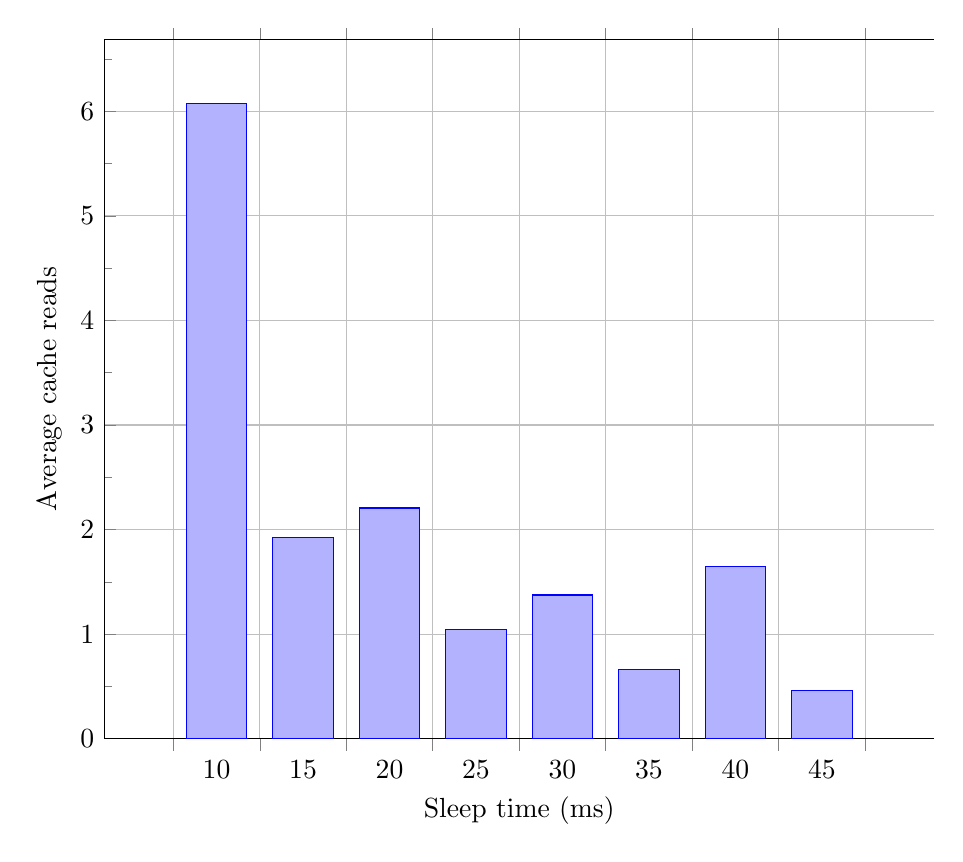
\begin{tikzpicture}
\begin{axis}
[
width=\resultsPlotWidthScale\textwidth,
axis y line*=left,
xlabel=Sleep time (ms),
ymin = 0,
%xmin = 0,
ylabel=Average cache reads,
%xtick={1, 2, 3, 4, 5, 6, 7, 8, 9},
%xticklabels={10, 15, 20, 25, 30, 35, 40, 45, 50},
%boxplot/draw direction=y,
%grid=both,
%ymajorgrids=true,
%yminorgrids=true,
ybar interval=0.7,
ymajorgrids=true,
%yminorgrids=true,
minor y tick num=1
%minor tick num=1
]
%\buildBoxPlot[black]{0}{0}{0}{0}{0}
%\buildBoxPlot[black]{0}{0}{0}{0}{0}
%\buildBoxPlot[black]{0}{0}{0}{0}{0}
%\buildBoxPlot[black]{0}{0}{0}{0}{0}
%\buildBoxPlot[black]{0}{0}{0}{0}{0}
%\buildBoxPlot[black]{0}{0}{0}{0}{0}
%\buildBoxPlot[black]{0}{0}{0}{0}{0}
%\buildBoxPlot[black]{0}{0}{0}{0}{0}
%\buildBoxPlot[black]{0}{0}{0}{0}{0}
\addplot coordinates {
	(10 ,6.076278918444858)
	(15 ,1.9250837336102817)
	(20 ,2.206446850393701)
	(25 ,1.044688862465319)
	(30 ,1.3747593094220163)
	(35 ,0.661782154722354)
	(40 ,1.6464805561590268)
	(45 ,0.46317152740208856)
	(50 ,1.858914282814271)
};

%matlab info
%     General model:
%     f(x) = (a/(x+b))+ c
%     Coefficients (with 95% confidence bounds):
%     a =       7.017  (-8.781, 22.82)
%     b =      -8.622  (-11.55, -5.697)
%     c =      0.9821  (0.01249, 1.952)
     
%\addplot[
%red,
%domain=10:50,
%samples=201,
%]
%{(7.017/(x-8.622))+ 0.9821};

\end{axis}
\end{tikzpicture}
	\caption{Decentralized solution with variable wait time cache reads experiment}
	\label{fig:exp:decen:sleep-cache}
\end{figure}

\FloatBarrier

\Cref{fig:exp:decen:sleep-cache} show that the average cache reads is declining when increasing the sleep time. As described in \cref{sec:cachereads}, cache reads only indicates if a given state has been read before, thus the number does not increase with the number times the same state has been read. Again, the 10 ms data point should be disregarded due to limited experiment equipment.
%, a fitted function of the plot has been put on top (red), the plot is in Matlab fitted against the function $\dfrac{a}{x + b} + c$.

\clearpage
\subsubsection{\nameref{subsec:Exper:perfom:2}}

\begin{figure}[h!]
	\centering
%	\begin{tikzpicture}
\begin{axis}
[
width=\textwidth,
axis y line*=left,
xlabel=Number of turbines,
ylabel=Regulation cycle time (ms),
ymin = 0,
xtick={1, 2, 3, 4, 5, 6, 7, 8, 9, 10, 11, 12, 13, 14, 15, 16, 17, 18, 19, 20},
xticklabels={5, 10, 15, 20, 25, 30, 35, 40, 45, 50, 55, 60, 65, 70, 75, 80, 85, 90, 95, 100},
boxplot/draw direction=y
]

%% /home/stefan/work/TestResults/Test5_Decentralized_success_12-4-2014_2100/nTurbines/DecentralizedLog0.csv
\buildBoxPlot{19.526002}{20.412002}{15.272001}{26.620001}{0.282}

%% /home/stefan/work/TestResults/Test5_Decentralized_success_12-4-2014_2100/nTurbines/DecentralizedLog1.csv
\buildBoxPlot{20.257002}{20.365001}{20.158001}{24.403002}{0.828002}

%% /home/stefan/work/TestResults/Test5_Decentralized_success_12-4-2014_2100/nTurbines/DecentralizedLog2.csv
\buildBoxPlot{20.221001}{20.311002}{20.126002}{24.641001}{3.778}

%% /home/stefan/work/TestResults/Test5_Decentralized_success_12-4-2014_2100/nTurbines/DecentralizedLog3.csv
\buildBoxPlot{20.203002}{20.321002}{20.066}{24.962}{0.246002}

%% /home/stefan/work/TestResults/Test5_Decentralized_success_12-4-2014_2100/nTurbines/DecentralizedLog4.csv
\buildBoxPlot{20.174001}{20.343}{19.946}{25.983002}{0.273002}

%% /home/stefan/work/TestResults/Test5_Decentralized_success_12-4-2014_2100/nTurbines/DecentralizedLog5.csv
\buildBoxPlot{20.190001}{20.286002}{20.051}{24.771001}{10.959001}

%% /home/stefan/work/TestResults/Test5_Decentralized_success_12-4-2014_2100/nTurbines/DecentralizedLog6.csv
\buildBoxPlot{20.079}{20.391001}{19.563001}{27.503001}{0.371002}

%% /home/stefan/work/TestResults/Test5_Decentralized_success_12-4-2014_2100/nTurbines/DecentralizedLog7.csv
\buildBoxPlot{20.176}{20.303001}{19.965}{30.63}{9.225}

%% /home/stefan/work/TestResults/Test5_Decentralized_success_12-4-2014_2100/nTurbines/DecentralizedLog8.csv
\buildBoxPlot{19.998}{20.351001}{19.215}{30.385002}{0.543001}

%% /home/stefan/work/TestResults/Test5_Decentralized_success_12-4-2014_2100/nTurbines/DecentralizedLog9.csv
\buildBoxPlot{20.008}{20.384001}{19.068001}{29.380001}{4.096002}

%% /home/stefan/work/TestResults/Test5_Decentralized_success_12-4-2014_2100/nTurbines/DecentralizedLog10.csv
\buildBoxPlot{19.902002}{20.353}{18.909001}{33.447001}{2.831002}

%% /home/stefan/work/TestResults/Test5_Decentralized_success_12-4-2014_2100/nTurbines/DecentralizedLog11.csv
\buildBoxPlot{19.937001}{20.373}{18.991001}{33.877001}{1.672002}

%% /home/stefan/work/TestResults/Test5_Decentralized_success_12-4-2014_2100/nTurbines/DecentralizedLog12.csv
\buildBoxPlot{20.056}{20.415001}{19.421002}{40.952001}{0.923001}

%% /home/stefan/work/TestResults/Test5_Decentralized_success_12-4-2014_2100/nTurbines/DecentralizedLog13.csv
\buildBoxPlot{20.215}{21.471}{19.378}{151.296001}{0.528001}

%% /home/stefan/work/TestResults/Test5_Decentralized_success_12-4-2014_2100/nTurbines/DecentralizedLog14.csv
\buildBoxPlot{19.920001}{20.535002}{18.897001}{53.699}{0.768}

%% /home/stefan/work/TestResults/Test5_Decentralized_success_12-4-2014_2100/nTurbines/DecentralizedLog15.csv
\buildBoxPlot{20.129002}{21.354002}{18.846002}{69.145001}{0.589001}

%% /home/stefan/work/TestResults/Test5_Decentralized_success_12-4-2014_2100/nTurbines/DecentralizedLog16.csv
\buildBoxPlot{20.189001}{22.247}{18.578001}{89.297001}{0.707}

%% /home/stefan/work/TestResults/Test5_Decentralized_success_12-4-2014_2100/nTurbines/DecentralizedLog17.csv
\buildBoxPlot{20.902001}{25.559001}{18.828}{142.836}{0.615001}

%% /home/stefan/work/TestResults/Test5_Decentralized_success_12-4-2014_2100/nTurbines/DecentralizedLog18.csv
\buildBoxPlot{25.609001}{35.368002}{20.078002}{150.034001}{0.579001}

%% /home/stefan/work/TestResults/Test5_Decentralized_success_12-4-2014_2100/nTurbines/DecentralizedLog19.csv
\buildBoxPlot{36.934001}{53.153001}{24.836001}{150.673002}{0.684001}


\addplot[thick, red!70] coordinates {
	(1 ,19.526002)
	(2 ,20.257002)
	(3 ,20.221001)
	(4 ,20.203002)
	(5 ,20.174001)
	(6 ,20.190001)
	(7 ,20.079)
	(8 ,20.176)
	(9 ,19.998)
	(10 ,20.008)
	(11 ,19.902002)
	(12 ,19.937001)
	(13 ,20.056)
	(14 ,20.215)
	(15 ,19.920001)
	(16 ,20.129002)
	(17 ,20.189001)
	(18 ,20.902001)
	(19 ,25.609001)
	(20 ,36.934001)
	
};

\end{axis}
\end{tikzpicture}
\begin{tikzpicture}
\begin{axis}
[
width=\textwidth,
axis y line*=left,
xlabel=Number of turbines,
ymin = 0,
ylabel=Average Cache hits,
xtick={1, 2, 3, 4, 5, 6, 7, 8, 9, 10, 11, 12, 13, 14, 15, 16, 17, 18, 19, 20},
xticklabels={5, 10, 15, 20, 25, 30, 35, 40, 45, 50, 55, 60, 65, 70, 75, 80, 85, 90, 95, 100},
boxplot/draw direction=y
]
\buildBoxPlot[black]{0}{0}{0}{0}{0}
\buildBoxPlot[black]{0}{0}{0}{0}{0}
\buildBoxPlot[black]{0}{0}{0}{0}{0}
\buildBoxPlot[black]{0}{0}{0}{0}{0}
\buildBoxPlot[black]{0}{0}{0}{0}{0}
\buildBoxPlot[black]{0}{0}{0}{0}{0}
\buildBoxPlot[black]{0}{0}{0}{0}{0}
\buildBoxPlot[black]{0}{0}{0}{0}{0}
\buildBoxPlot[black]{0}{0}{0}{0}{0}
\buildBoxPlot[black]{0}{0}{0}{0}{0}
\buildBoxPlot[black]{0}{0}{0}{0}{0}
\buildBoxPlot[black]{0}{0}{0}{0}{0}
\buildBoxPlot[black]{0}{0}{0}{0}{0}
\buildBoxPlot[black]{0}{0}{0}{0}{0}
\buildBoxPlot[black]{0}{0}{0}{0}{0}
\buildBoxPlot[black]{0}{0}{0}{0}{0}
\buildBoxPlot[black]{0}{0}{0}{0}{0}
\buildBoxPlot[black]{0}{0}{0}{0}{0}
\buildBoxPlot[black]{0}{0}{0}{0}{0}
\buildBoxPlot[black]{0}{0}{0}{0}{0}
\addplot[thick, orange!70] coordinates {
	(1 ,0.2591015249347438)
	(2 ,0.3423283799799435)
	(3 ,0.4286200856364344)
	(4 ,0.7913519050319182)
	(5 ,1.171919068056407)
	(6 ,0.4440826120490188)
	(7 ,1.8595523144717856)
	(8 ,0.506366007056297)
	(9 ,1.8951768000539848)
	(10 ,2.037951753081981)
	(11 ,2.0728170589196186)
	(12 ,2.0275369832294468)
	(13 ,1.2416290071090674)
	(14 ,3.5220372523313626)
	(15 ,2.115832267020478)
	(16 ,3.7417427229878832)
	(17 ,5.311682134712245)
	(18 ,8.473847137142263)
	(19 ,14.663734246038112)
	(20 ,22.06932793366117)
};
\end{axis}
\end{tikzpicture}
	% This file was created by matlab2tikz.
% Minimal pgfplots version: 1.3
%
%The latest updates can be retrieved from
%  http://www.mathworks.com/matlabcentral/fileexchange/22022-matlab2tikz
%where you can also make suggestions and rate matlab2tikz.
%
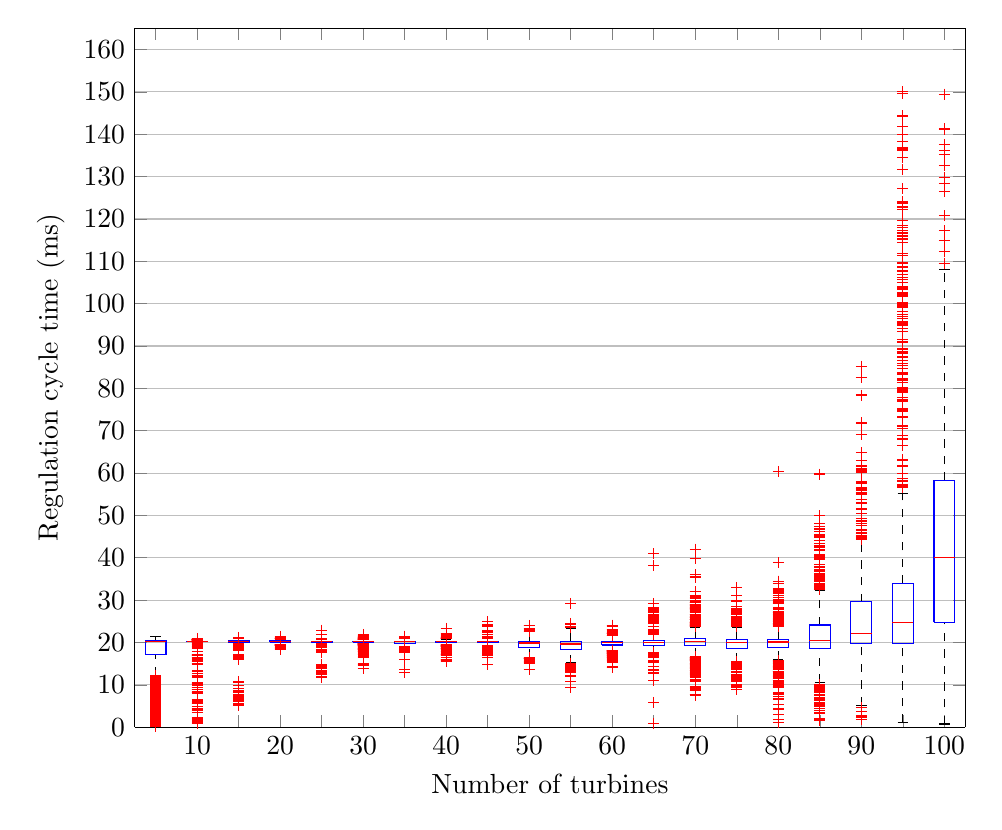
\begin{tikzpicture}

\begin{axis}[%
	width=\resultsPlotWidthScale\textwidth,
	separate axis lines,
	xlabel=Number of turbines,
	ylabel=Regulation cycle time (ms),	
	xmin=0.5,
	xmax=20.5,
	max space between ticks=17.5,
	xtick=			{1, 2, 3, 4, 5, 6, 7, 8, 9, 10, 11, 12, 13, 14, 15, 16, 17, 18, 19, 20},
	xticklabels={, 10, , 20, , 30, , 40,  , 50,   , 60,   , 70,   , 80,   , 90,  , 100},
	ymin=0,
	ymajorgrids=true,
	yminorgrids=true	
]
\addplot [color=black,dashed,forget plot]
  table[row sep=crcr]{%
1	20.4880015\\
1	21.315\\
};
\addplot [color=black,dashed,forget plot]
  table[row sep=crcr]{%
2	20.312501\\
2	20.526\\
};
\addplot [color=black,dashed,forget plot]
  table[row sep=crcr]{%
3	20.405501\\
3	20.839001\\
};
\addplot [color=black,dashed,forget plot]
  table[row sep=crcr]{%
4	20.3405015\\
4	20.805\\
};
\addplot [color=black,dashed,forget plot]
  table[row sep=crcr]{%
5	20.292001\\
5	20.604002\\
};
\addplot [color=black,dashed,forget plot]
  table[row sep=crcr]{%
6	20.3220005\\
6	20.633001\\
};
\addplot [color=black,dashed,forget plot]
  table[row sep=crcr]{%
7	20.2860015\\
7	20.969\\
};
\addplot [color=black,dashed,forget plot]
  table[row sep=crcr]{%
8	20.315001\\
8	20.815\\
};
\addplot [color=black,dashed,forget plot]
  table[row sep=crcr]{%
9	20.311001\\
9	20.895002\\
};
\addplot [color=black,dashed,forget plot]
  table[row sep=crcr]{%
10	20.2740005\\
10	22.548001\\
};
\addplot [color=black,dashed,forget plot]
  table[row sep=crcr]{%
11	20.325\\
11	23.385002\\
};
\addplot [color=black,dashed,forget plot]
  table[row sep=crcr]{%
12	20.289502\\
12	21.569001\\
};
\addplot [color=black,dashed,forget plot]
  table[row sep=crcr]{%
13	20.386501\\
13	21.981002\\
};
\addplot [color=black,dashed,forget plot]
  table[row sep=crcr]{%
14	21.027001\\
14	23.521001\\
};
\addplot [color=black,dashed,forget plot]
  table[row sep=crcr]{%
15	20.6225015\\
15	23.646001\\
};
\addplot [color=black,dashed,forget plot]
  table[row sep=crcr]{%
16	20.771001\\
16	23.726001\\
};
\addplot [color=black,dashed,forget plot]
  table[row sep=crcr]{%
17	24.128002\\
17	32.259002\\
};
\addplot [color=black,dashed,forget plot]
  table[row sep=crcr]{%
18	29.602502\\
18	44.273002\\
};
\addplot [color=black,dashed,forget plot]
  table[row sep=crcr]{%
19	33.9330015\\
19	55.095001\\
};
\addplot [color=black,dashed,forget plot]
  table[row sep=crcr]{%
20	58.175501\\
20	108.037001\\
};
\addplot [color=black,dashed,forget plot]
  table[row sep=crcr]{%
1	12.261002\\
1	17.1955015\\
};
\addplot [color=black,dashed,forget plot]
  table[row sep=crcr]{%
2	19.955001\\
2	20.1680005\\
};
\addplot [color=black,dashed,forget plot]
  table[row sep=crcr]{%
3	19.700001\\
3	20.1150005\\
};
\addplot [color=black,dashed,forget plot]
  table[row sep=crcr]{%
4	19.565\\
4	20.0290015\\
};
\addplot [color=black,dashed,forget plot]
  table[row sep=crcr]{%
5	19.763001\\
5	20.079001\\
};
\addplot [color=black,dashed,forget plot]
  table[row sep=crcr]{%
6	19.802001\\
6	20.108001\\
};
\addplot [color=black,dashed,forget plot]
  table[row sep=crcr]{%
7	19.151\\
7	19.830501\\
};
\addplot [color=black,dashed,forget plot]
  table[row sep=crcr]{%
8	19.491002\\
8	19.979002\\
};
\addplot [color=black,dashed,forget plot]
  table[row sep=crcr]{%
9	19.339\\
9	19.920501\\
};
\addplot [color=black,dashed,forget plot]
  table[row sep=crcr]{%
10	16.402001\\
10	18.723001\\
};
\addplot [color=black,dashed,forget plot]
  table[row sep=crcr]{%
11	15.179001\\
11	18.2495015\\
};
\addplot [color=black,dashed,forget plot]
  table[row sep=crcr]{%
12	18.128001\\
12	19.4080015\\
};
\addplot [color=black,dashed,forget plot]
  table[row sep=crcr]{%
13	17.723002\\
13	19.314502\\
};
\addplot [color=black,dashed,forget plot]
  table[row sep=crcr]{%
14	16.626001\\
14	19.263001\\
};
\addplot [color=black,dashed,forget plot]
  table[row sep=crcr]{%
15	15.513001\\
15	18.577001\\
};
\addplot [color=black,dashed,forget plot]
  table[row sep=crcr]{%
16	15.921001\\
16	18.8005\\
};
\addplot [color=black,dashed,forget plot]
  table[row sep=crcr]{%
17	10.532001\\
17	18.668502\\
};
\addplot [color=black,dashed,forget plot]
  table[row sep=crcr]{%
18	5.197002\\
18	19.750002\\
};
\addplot [color=black,dashed,forget plot]
  table[row sep=crcr]{%
19	1.037001\\
19	19.768001\\
};
\addplot [color=black,dashed,forget plot]
  table[row sep=crcr]{%
20	0.753001\\
20	24.7620015\\
};
\addplot [color=black,solid,forget plot]
  table[row sep=crcr]{%
0.875	21.315\\
1.125	21.315\\
};
\addplot [color=black,solid,forget plot]
  table[row sep=crcr]{%
1.875	20.526\\
2.125	20.526\\
};
\addplot [color=black,solid,forget plot]
  table[row sep=crcr]{%
2.875	20.839001\\
3.125	20.839001\\
};
\addplot [color=black,solid,forget plot]
  table[row sep=crcr]{%
3.875	20.805\\
4.125	20.805\\
};
\addplot [color=black,solid,forget plot]
  table[row sep=crcr]{%
4.875	20.604002\\
5.125	20.604002\\
};
\addplot [color=black,solid,forget plot]
  table[row sep=crcr]{%
5.875	20.633001\\
6.125	20.633001\\
};
\addplot [color=black,solid,forget plot]
  table[row sep=crcr]{%
6.875	20.969\\
7.125	20.969\\
};
\addplot [color=black,solid,forget plot]
  table[row sep=crcr]{%
7.875	20.815\\
8.125	20.815\\
};
\addplot [color=black,solid,forget plot]
  table[row sep=crcr]{%
8.875	20.895002\\
9.125	20.895002\\
};
\addplot [color=black,solid,forget plot]
  table[row sep=crcr]{%
9.875	22.548001\\
10.125	22.548001\\
};
\addplot [color=black,solid,forget plot]
  table[row sep=crcr]{%
10.875	23.385002\\
11.125	23.385002\\
};
\addplot [color=black,solid,forget plot]
  table[row sep=crcr]{%
11.875	21.569001\\
12.125	21.569001\\
};
\addplot [color=black,solid,forget plot]
  table[row sep=crcr]{%
12.875	21.981002\\
13.125	21.981002\\
};
\addplot [color=black,solid,forget plot]
  table[row sep=crcr]{%
13.875	23.521001\\
14.125	23.521001\\
};
\addplot [color=black,solid,forget plot]
  table[row sep=crcr]{%
14.875	23.646001\\
15.125	23.646001\\
};
\addplot [color=black,solid,forget plot]
  table[row sep=crcr]{%
15.875	23.726001\\
16.125	23.726001\\
};
\addplot [color=black,solid,forget plot]
  table[row sep=crcr]{%
16.875	32.259002\\
17.125	32.259002\\
};
\addplot [color=black,solid,forget plot]
  table[row sep=crcr]{%
17.875	44.273002\\
18.125	44.273002\\
};
\addplot [color=black,solid,forget plot]
  table[row sep=crcr]{%
18.875	55.095001\\
19.125	55.095001\\
};
\addplot [color=black,solid,forget plot]
  table[row sep=crcr]{%
19.875	108.037001\\
20.125	108.037001\\
};
\addplot [color=black,solid,forget plot]
  table[row sep=crcr]{%
0.875	12.261002\\
1.125	12.261002\\
};
\addplot [color=black,solid,forget plot]
  table[row sep=crcr]{%
1.875	19.955001\\
2.125	19.955001\\
};
\addplot [color=black,solid,forget plot]
  table[row sep=crcr]{%
2.875	19.700001\\
3.125	19.700001\\
};
\addplot [color=black,solid,forget plot]
  table[row sep=crcr]{%
3.875	19.565\\
4.125	19.565\\
};
\addplot [color=black,solid,forget plot]
  table[row sep=crcr]{%
4.875	19.763001\\
5.125	19.763001\\
};
\addplot [color=black,solid,forget plot]
  table[row sep=crcr]{%
5.875	19.802001\\
6.125	19.802001\\
};
\addplot [color=black,solid,forget plot]
  table[row sep=crcr]{%
6.875	19.151\\
7.125	19.151\\
};
\addplot [color=black,solid,forget plot]
  table[row sep=crcr]{%
7.875	19.491002\\
8.125	19.491002\\
};
\addplot [color=black,solid,forget plot]
  table[row sep=crcr]{%
8.875	19.339\\
9.125	19.339\\
};
\addplot [color=black,solid,forget plot]
  table[row sep=crcr]{%
9.875	16.402001\\
10.125	16.402001\\
};
\addplot [color=black,solid,forget plot]
  table[row sep=crcr]{%
10.875	15.179001\\
11.125	15.179001\\
};
\addplot [color=black,solid,forget plot]
  table[row sep=crcr]{%
11.875	18.128001\\
12.125	18.128001\\
};
\addplot [color=black,solid,forget plot]
  table[row sep=crcr]{%
12.875	17.723002\\
13.125	17.723002\\
};
\addplot [color=black,solid,forget plot]
  table[row sep=crcr]{%
13.875	16.626001\\
14.125	16.626001\\
};
\addplot [color=black,solid,forget plot]
  table[row sep=crcr]{%
14.875	15.513001\\
15.125	15.513001\\
};
\addplot [color=black,solid,forget plot]
  table[row sep=crcr]{%
15.875	15.921001\\
16.125	15.921001\\
};
\addplot [color=black,solid,forget plot]
  table[row sep=crcr]{%
16.875	10.532001\\
17.125	10.532001\\
};
\addplot [color=black,solid,forget plot]
  table[row sep=crcr]{%
17.875	5.197002\\
18.125	5.197002\\
};
\addplot [color=black,solid,forget plot]
  table[row sep=crcr]{%
18.875	1.037001\\
19.125	1.037001\\
};
\addplot [color=black,solid,forget plot]
  table[row sep=crcr]{%
19.875	0.753001\\
20.125	0.753001\\
};
\addplot [color=blue,solid,forget plot]
  table[row sep=crcr]{%
0.75	17.1955015\\
0.75	20.4880015\\
1.25	20.4880015\\
1.25	17.1955015\\
0.75	17.1955015\\
};
\addplot [color=blue,solid,forget plot]
  table[row sep=crcr]{%
1.75	20.1680005\\
1.75	20.312501\\
2.25	20.312501\\
2.25	20.1680005\\
1.75	20.1680005\\
};
\addplot [color=blue,solid,forget plot]
  table[row sep=crcr]{%
2.75	20.1150005\\
2.75	20.405501\\
3.25	20.405501\\
3.25	20.1150005\\
2.75	20.1150005\\
};
\addplot [color=blue,solid,forget plot]
  table[row sep=crcr]{%
3.75	20.0290015\\
3.75	20.3405015\\
4.25	20.3405015\\
4.25	20.0290015\\
3.75	20.0290015\\
};
\addplot [color=blue,solid,forget plot]
  table[row sep=crcr]{%
4.75	20.079001\\
4.75	20.292001\\
5.25	20.292001\\
5.25	20.079001\\
4.75	20.079001\\
};
\addplot [color=blue,solid,forget plot]
  table[row sep=crcr]{%
5.75	20.108001\\
5.75	20.3220005\\
6.25	20.3220005\\
6.25	20.108001\\
5.75	20.108001\\
};
\addplot [color=blue,solid,forget plot]
  table[row sep=crcr]{%
6.75	19.830501\\
6.75	20.2860015\\
7.25	20.2860015\\
7.25	19.830501\\
6.75	19.830501\\
};
\addplot [color=blue,solid,forget plot]
  table[row sep=crcr]{%
7.75	19.979002\\
7.75	20.315001\\
8.25	20.315001\\
8.25	19.979002\\
7.75	19.979002\\
};
\addplot [color=blue,solid,forget plot]
  table[row sep=crcr]{%
8.75	19.920501\\
8.75	20.311001\\
9.25	20.311001\\
9.25	19.920501\\
8.75	19.920501\\
};
\addplot [color=blue,solid,forget plot]
  table[row sep=crcr]{%
9.75	18.723001\\
9.75	20.2740005\\
10.25	20.2740005\\
10.25	18.723001\\
9.75	18.723001\\
};
\addplot [color=blue,solid,forget plot]
  table[row sep=crcr]{%
10.75	18.2495015\\
10.75	20.325\\
11.25	20.325\\
11.25	18.2495015\\
10.75	18.2495015\\
};
\addplot [color=blue,solid,forget plot]
  table[row sep=crcr]{%
11.75	19.4080015\\
11.75	20.289502\\
12.25	20.289502\\
12.25	19.4080015\\
11.75	19.4080015\\
};
\addplot [color=blue,solid,forget plot]
  table[row sep=crcr]{%
12.75	19.314502\\
12.75	20.386501\\
13.25	20.386501\\
13.25	19.314502\\
12.75	19.314502\\
};
\addplot [color=blue,solid,forget plot]
  table[row sep=crcr]{%
13.75	19.263001\\
13.75	21.027001\\
14.25	21.027001\\
14.25	19.263001\\
13.75	19.263001\\
};
\addplot [color=blue,solid,forget plot]
  table[row sep=crcr]{%
14.75	18.577001\\
14.75	20.6225015\\
15.25	20.6225015\\
15.25	18.577001\\
14.75	18.577001\\
};
\addplot [color=blue,solid,forget plot]
  table[row sep=crcr]{%
15.75	18.8005\\
15.75	20.771001\\
16.25	20.771001\\
16.25	18.8005\\
15.75	18.8005\\
};
\addplot [color=blue,solid,forget plot]
  table[row sep=crcr]{%
16.75	18.668502\\
16.75	24.128002\\
17.25	24.128002\\
17.25	18.668502\\
16.75	18.668502\\
};
\addplot [color=blue,solid,forget plot]
  table[row sep=crcr]{%
17.75	19.750002\\
17.75	29.602502\\
18.25	29.602502\\
18.25	19.750002\\
17.75	19.750002\\
};
\addplot [color=blue,solid,forget plot]
  table[row sep=crcr]{%
18.75	19.768001\\
18.75	33.9330015\\
19.25	33.9330015\\
19.25	19.768001\\
18.75	19.768001\\
};
\addplot [color=blue,solid,forget plot]
  table[row sep=crcr]{%
19.75	24.7620015\\
19.75	58.175501\\
20.25	58.175501\\
20.25	24.7620015\\
19.75	24.7620015\\
};
\addplot [color=red,solid,forget plot]
  table[row sep=crcr]{%
0.75	20.311001\\
1.25	20.311001\\
};
\addplot [color=red,solid,forget plot]
  table[row sep=crcr]{%
1.75	20.231001\\
2.25	20.231001\\
};
\addplot [color=red,solid,forget plot]
  table[row sep=crcr]{%
2.75	20.261\\
3.25	20.261\\
};
\addplot [color=red,solid,forget plot]
  table[row sep=crcr]{%
3.75	20.1890015\\
4.25	20.1890015\\
};
\addplot [color=red,solid,forget plot]
  table[row sep=crcr]{%
4.75	20.1940015\\
5.25	20.1940015\\
};
\addplot [color=red,solid,forget plot]
  table[row sep=crcr]{%
5.75	20.221001\\
6.25	20.221001\\
};
\addplot [color=red,solid,forget plot]
  table[row sep=crcr]{%
6.75	20.141002\\
7.25	20.141002\\
};
\addplot [color=red,solid,forget plot]
  table[row sep=crcr]{%
7.75	20.205501\\
8.25	20.205501\\
};
\addplot [color=red,solid,forget plot]
  table[row sep=crcr]{%
8.75	20.16\\
9.25	20.16\\
};
\addplot [color=red,solid,forget plot]
  table[row sep=crcr]{%
9.75	19.8785\\
10.25	19.8785\\
};
\addplot [color=red,solid,forget plot]
  table[row sep=crcr]{%
10.75	19.6445005\\
11.25	19.6445005\\
};
\addplot [color=red,solid,forget plot]
  table[row sep=crcr]{%
11.75	19.965501\\
12.25	19.965501\\
};
\addplot [color=red,solid,forget plot]
  table[row sep=crcr]{%
12.75	20.005501\\
13.25	20.005501\\
};
\addplot [color=red,solid,forget plot]
  table[row sep=crcr]{%
13.75	20.1585015\\
14.25	20.1585015\\
};
\addplot [color=red,solid,forget plot]
  table[row sep=crcr]{%
14.75	20.0240015\\
15.25	20.0240015\\
};
\addplot [color=red,solid,forget plot]
  table[row sep=crcr]{%
15.75	20.1070015\\
16.25	20.1070015\\
};
\addplot [color=red,solid,forget plot]
  table[row sep=crcr]{%
16.75	20.438502\\
17.25	20.438502\\
};
\addplot [color=red,solid,forget plot]
  table[row sep=crcr]{%
17.75	22.1250015\\
18.25	22.1250015\\
};
\addplot [color=red,solid,forget plot]
  table[row sep=crcr]{%
18.75	24.696001\\
19.25	24.696001\\
};
\addplot [color=red,solid,forget plot]
  table[row sep=crcr]{%
19.75	40.1645005\\
20.25	40.1645005\\
};
\addplot [color=blue,only marks,mark=+,mark options={solid,draw=red},forget plot]
  table[row sep=crcr]{%
1	0.282\\
1	0.385\\
1	0.471\\
1	0.491\\
1	0.595\\
1	0.625\\
1	0.626\\
1	0.788\\
1	1.127\\
1	1.291002\\
1	1.307\\
1	1.563\\
1	1.580001\\
1	1.597\\
1	1.669002\\
1	1.752002\\
1	1.840002\\
1	2.053001\\
1	2.078002\\
1	2.080001\\
1	2.085002\\
1	2.111001\\
1	2.189001\\
1	2.202001\\
1	2.319002\\
1	2.329002\\
1	2.352\\
1	2.361001\\
1	2.442\\
1	2.457\\
1	2.559\\
1	2.702001\\
1	2.71\\
1	2.818\\
1	2.922001\\
1	3.205001\\
1	3.22\\
1	3.305\\
1	3.307\\
1	3.314\\
1	3.333\\
1	3.339\\
1	3.408001\\
1	3.541001\\
1	3.600002\\
1	3.629002\\
1	3.642001\\
1	3.764001\\
1	3.769002\\
1	3.875002\\
1	3.881001\\
1	3.947001\\
1	3.962001\\
1	4.000001\\
1	4.057001\\
1	4.084002\\
1	4.101001\\
1	4.110001\\
1	4.144001\\
1	4.325001\\
1	4.379001\\
1	4.426001\\
1	4.438001\\
1	4.442002\\
1	4.448001\\
1	4.499001\\
1	4.510001\\
1	4.544001\\
1	4.563002\\
1	4.576001\\
1	4.580001\\
1	4.593001\\
1	4.628001\\
1	4.660001\\
1	4.684001\\
1	4.685001\\
1	4.722001\\
1	4.822001\\
1	4.861001\\
1	4.876001\\
1	4.889001\\
1	4.949001\\
1	4.991001\\
1	4.998001\\
1	5.003001\\
1	5.016001\\
1	5.029001\\
1	5.060001\\
1	5.098001\\
1	5.105001\\
1	5.196001\\
1	5.205001\\
1	5.220001\\
1	5.257001\\
1	5.299001\\
1	5.362001\\
1	5.373001\\
1	5.400002\\
1	5.523001\\
1	5.625001\\
1	5.777001\\
1	5.835002\\
1	5.876001\\
1	6.015001\\
1	6.204001\\
1	6.24\\
1	6.296\\
1	6.366002\\
1	6.461001\\
1	6.683001\\
1	6.716001\\
1	6.771002\\
1	6.881\\
1	6.907\\
1	7.06\\
1	7.116001\\
1	7.13\\
1	7.16\\
1	7.179\\
1	7.193001\\
1	7.316\\
1	7.497\\
1	7.592001\\
1	7.627001\\
1	7.796001\\
1	7.802002\\
1	7.886\\
1	7.892\\
1	8.083\\
1	8.123002\\
1	8.182001\\
1	8.289002\\
1	8.294002\\
1	8.321\\
1	8.531\\
1	8.659\\
1	8.710002\\
1	8.906\\
1	8.944001\\
1	8.964\\
1	9.073002\\
1	9.181\\
1	9.278\\
1	9.326002\\
1	9.518\\
1	9.875\\
1	10.140002\\
1	10.195\\
1	10.383002\\
1	10.614\\
1	10.658002\\
1	10.712002\\
1	10.853002\\
1	10.856002\\
1	10.983\\
1	10.987002\\
1	11.284002\\
1	11.298001\\
1	11.558001\\
1	11.583002\\
1	11.776\\
1	11.857001\\
1	12.063\\
1	12.202002\\
};
\addplot [color=blue,only marks,mark=+,mark options={solid,draw=red},forget plot]
  table[row sep=crcr]{%
2	0.929\\
2	1.047\\
2	1.407\\
2	1.588\\
2	1.728\\
2	2.129\\
2	2.3\\
2	3.459002\\
2	3.954002\\
2	4.153002\\
2	4.419002\\
2	4.953002\\
2	5.539001\\
2	5.625001\\
2	5.835001\\
2	6.045001\\
2	6.428001\\
2	8.074\\
2	8.174\\
2	8.252\\
2	8.527\\
2	8.895002\\
2	8.957001\\
2	9.336002\\
2	9.38\\
2	9.968\\
2	10.298\\
2	10.392\\
2	10.575001\\
2	11.657\\
2	12.094\\
2	12.302\\
2	12.763\\
2	13.111002\\
2	13.465002\\
2	14.828002\\
2	15.041002\\
2	15.088002\\
2	15.465001\\
2	15.526\\
2	15.662\\
2	16.028001\\
2	16.086001\\
2	16.516002\\
2	16.548002\\
2	16.824\\
2	16.890001\\
2	16.921001\\
2	17.024001\\
2	17.164001\\
2	17.169001\\
2	17.183001\\
2	17.206001\\
2	17.785001\\
2	18.500001\\
2	18.834001\\
2	19.024001\\
2	19.090001\\
2	19.198001\\
2	19.538\\
2	19.542001\\
2	19.654\\
2	19.897001\\
2	19.94\\
2	19.943001\\
2	19.951002\\
2	20.53\\
2	20.530001\\
2	20.538\\
2	20.538\\
2	20.538001\\
2	20.541002\\
2	20.542002\\
2	20.542002\\
2	20.558\\
2	20.56\\
2	20.560001\\
2	20.565001\\
2	20.567\\
2	20.568\\
2	20.569002\\
2	20.579\\
2	20.585001\\
2	20.588\\
2	20.592\\
2	20.595002\\
2	20.599002\\
2	20.6\\
2	20.6\\
2	20.601002\\
2	20.61\\
2	20.613\\
2	20.614001\\
2	20.623\\
2	20.625001\\
2	20.629002\\
2	20.632\\
2	20.634001\\
2	20.642001\\
2	20.654\\
2	20.655\\
2	20.666\\
2	20.672\\
2	20.684\\
2	20.706\\
2	20.708\\
2	20.710001\\
2	20.712\\
2	20.713002\\
2	20.726001\\
2	20.757\\
2	20.76\\
2	20.776\\
2	20.785001\\
2	20.802\\
2	20.847\\
2	20.867002\\
2	20.893\\
2	20.925\\
};
\addplot [color=blue,only marks,mark=+,mark options={solid,draw=red},forget plot]
  table[row sep=crcr]{%
3	5.013001\\
3	5.135001\\
3	5.143001\\
3	5.174001\\
3	5.198\\
3	5.205001\\
3	5.225001\\
3	5.242\\
3	5.295\\
3	5.336001\\
3	5.349\\
3	5.399\\
3	5.450001\\
3	5.459001\\
3	5.483001\\
3	5.526\\
3	5.612001\\
3	5.988001\\
3	6.318\\
3	6.396001\\
3	6.412002\\
3	6.619002\\
3	6.694002\\
3	6.750002\\
3	6.848002\\
3	6.856001\\
3	6.921001\\
3	6.923001\\
3	6.926002\\
3	6.998001\\
3	7.022001\\
3	7.050001\\
3	7.168001\\
3	7.303001\\
3	7.348001\\
3	7.379\\
3	7.431\\
3	7.541001\\
3	7.671001\\
3	8.195001\\
3	8.540001\\
3	9.028001\\
3	9.860001\\
3	10.653001\\
3	10.748001\\
3	10.825001\\
3	16.071001\\
3	16.100001\\
3	16.284\\
3	16.339001\\
3	16.357001\\
3	16.397001\\
3	16.438001\\
3	16.463\\
3	16.537001\\
3	16.552001\\
3	16.626001\\
3	16.935001\\
3	16.943001\\
3	17.077001\\
3	17.238001\\
3	18.041002\\
3	18.374002\\
3	18.541002\\
3	18.874002\\
3	18.969002\\
3	19.328001\\
3	19.389001\\
3	19.528\\
3	19.532\\
3	19.569\\
3	19.633001\\
3	20.845\\
3	20.847\\
3	20.904\\
3	20.913\\
3	20.938\\
3	20.941001\\
3	20.944001\\
3	20.965001\\
3	20.965001\\
3	20.973002\\
3	20.987001\\
3	21.025001\\
3	21.068\\
3	21.081\\
3	21.180001\\
};
\addplot [color=blue,only marks,mark=+,mark options={solid,draw=red},forget plot]
  table[row sep=crcr]{%
4	18.351\\
4	18.364001\\
4	18.462001\\
4	18.510001\\
4	18.811001\\
4	18.815\\
4	19.062\\
4	19.202\\
4	19.204001\\
4	19.27\\
4	19.271001\\
4	19.274\\
4	19.310001\\
4	19.311001\\
4	19.331001\\
4	19.372\\
4	19.375001\\
4	19.380001\\
4	19.386001\\
4	19.393001\\
4	19.450001\\
4	19.479001\\
4	19.479002\\
4	19.495001\\
4	19.498001\\
4	19.513\\
4	19.515002\\
4	19.521002\\
4	19.522001\\
4	19.530001\\
4	19.559001\\
4	20.822\\
4	20.836\\
4	20.842\\
4	20.842001\\
4	20.845\\
4	20.872\\
4	20.913002\\
4	20.97\\
4	20.977001\\
4	20.984\\
4	21.143\\
4	21.166002\\
4	21.461002\\
};
\addplot [color=blue,only marks,mark=+,mark options={solid,draw=red},forget plot]
  table[row sep=crcr]{%
5	11.850002\\
5	12.356001\\
5	12.736001\\
5	12.928\\
5	13.008\\
5	13.251\\
5	13.858002\\
5	13.878\\
5	13.890002\\
5	13.900001\\
5	13.963001\\
5	14.080001\\
5	14.130001\\
5	14.163002\\
5	14.181001\\
5	14.185002\\
5	14.208001\\
5	14.233001\\
5	14.252002\\
5	14.257002\\
5	14.367001\\
5	14.456001\\
5	14.516001\\
5	14.560001\\
5	14.593001\\
5	14.617\\
5	14.620001\\
5	14.622\\
5	14.647001\\
5	14.713001\\
5	14.756001\\
5	17.591\\
5	17.782002\\
5	17.785001\\
5	18.065002\\
5	18.135001\\
5	18.220002\\
5	18.235\\
5	18.238\\
5	18.240001\\
5	18.316001\\
5	18.350001\\
5	18.774001\\
5	18.928001\\
5	18.963001\\
5	19.042001\\
5	19.068\\
5	19.096001\\
5	19.099001\\
5	19.102001\\
5	19.153\\
5	19.206002\\
5	19.226001\\
5	19.232\\
5	19.315002\\
5	19.320001\\
5	19.324002\\
5	19.341001\\
5	19.395001\\
5	19.396001\\
5	19.451002\\
5	19.472001\\
5	19.483001\\
5	19.496001\\
5	19.506001\\
5	19.519001\\
5	19.532002\\
5	19.535001\\
5	19.537002\\
5	19.538002\\
5	19.542001\\
5	19.580002\\
5	19.6\\
5	19.627001\\
5	19.652002\\
5	19.653001\\
5	19.654001\\
5	19.654002\\
5	19.662002\\
5	19.666002\\
5	19.680001\\
5	19.691002\\
5	19.701001\\
5	19.702002\\
5	19.705002\\
5	19.712001\\
5	19.721001\\
5	19.735002\\
5	19.737002\\
5	19.745001\\
5	19.751001\\
5	20.621001\\
5	20.636\\
5	20.677002\\
5	20.723\\
5	20.772\\
5	20.825\\
5	20.837\\
5	20.960001\\
5	21.796001\\
5	22.921001\\
};
\addplot [color=blue,only marks,mark=+,mark options={solid,draw=red},forget plot]
  table[row sep=crcr]{%
6	13.851001\\
6	14.613001\\
6	14.747\\
6	14.894\\
6	14.966\\
6	16.553001\\
6	16.696001\\
6	17.046001\\
6	17.103\\
6	17.402001\\
6	17.547001\\
6	17.802001\\
6	17.908001\\
6	17.917001\\
6	17.943001\\
6	18.012002\\
6	18.092\\
6	18.276002\\
6	18.284\\
6	18.296\\
6	18.306001\\
6	18.343002\\
6	18.370001\\
6	18.389002\\
6	18.414001\\
6	18.502001\\
6	18.554\\
6	18.558001\\
6	18.646001\\
6	18.655001\\
6	18.656\\
6	18.671\\
6	18.679\\
6	18.725001\\
6	18.767001\\
6	18.780001\\
6	18.882001\\
6	18.941\\
6	19.009002\\
6	19.014001\\
6	19.019002\\
6	19.119001\\
6	19.154\\
6	19.154001\\
6	19.181\\
6	19.184001\\
6	19.199001\\
6	19.228001\\
6	19.291001\\
6	19.296\\
6	19.338001\\
6	19.351002\\
6	19.380001\\
6	19.380001\\
6	19.417002\\
6	19.423001\\
6	19.451\\
6	19.457002\\
6	19.465002\\
6	19.473001\\
6	19.490001\\
6	19.507001\\
6	19.513\\
6	19.521002\\
6	19.534001\\
6	19.554001\\
6	19.557\\
6	19.558001\\
6	19.562\\
6	19.564001\\
6	19.577\\
6	19.597\\
6	19.598001\\
6	19.605002\\
6	19.625001\\
6	19.640001\\
6	19.646\\
6	19.652\\
6	19.672001\\
6	19.676001\\
6	19.683001\\
6	19.691\\
6	19.698\\
6	19.707\\
6	19.711\\
6	19.712001\\
6	19.712001\\
6	19.714002\\
6	19.718001\\
6	19.719001\\
6	19.723\\
6	19.728\\
6	19.735001\\
6	19.744002\\
6	19.776001\\
6	20.661001\\
6	20.667001\\
6	20.682002\\
6	20.695001\\
6	20.709001\\
6	20.720001\\
6	20.734001\\
6	20.735001\\
6	20.736\\
6	20.738001\\
6	20.741\\
6	20.742001\\
6	20.742001\\
6	20.744\\
6	20.817002\\
6	20.848001\\
6	20.848001\\
6	20.866001\\
6	20.869001\\
6	20.884002\\
6	20.89\\
6	20.892002\\
6	20.903001\\
6	20.931002\\
6	20.955002\\
6	21.023002\\
6	21.048001\\
6	21.063002\\
6	21.065\\
6	21.097002\\
6	21.154002\\
6	21.169002\\
6	21.195001\\
6	21.267001\\
6	21.327001\\
6	21.375001\\
6	21.488001\\
6	21.491002\\
6	21.585001\\
6	21.610002\\
6	21.922002\\
};
\addplot [color=blue,only marks,mark=+,mark options={solid,draw=red},forget plot]
  table[row sep=crcr]{%
7	12.820002\\
7	13.599\\
7	15.88\\
7	17.569002\\
7	17.635\\
7	17.935\\
7	18.048\\
7	18.101\\
7	18.199\\
7	18.261\\
7	18.319002\\
7	18.355\\
7	18.372\\
7	18.382002\\
7	18.42\\
7	18.438\\
7	18.444002\\
7	18.470002\\
7	18.495\\
7	18.502002\\
7	18.684001\\
7	18.699\\
7	18.706001\\
7	18.717002\\
7	18.723\\
7	18.727\\
7	18.735002\\
7	18.746\\
7	18.755\\
7	18.794001\\
7	18.875002\\
7	18.895\\
7	18.905\\
7	18.931001\\
7	18.942\\
7	18.950001\\
7	18.952\\
7	18.962\\
7	18.974\\
7	18.988002\\
7	19.013002\\
7	19.024\\
7	19.028001\\
7	19.042\\
7	19.046\\
7	19.048002\\
7	19.052002\\
7	19.057\\
7	19.065\\
7	19.07\\
7	19.085\\
7	19.086\\
7	19.106002\\
7	19.129001\\
7	19.132001\\
7	19.136\\
7	19.136\\
7	19.14\\
7	19.145001\\
7	20.976002\\
7	20.984\\
7	20.988\\
7	21.019\\
7	21.045\\
7	21.047002\\
7	21.066\\
7	21.135002\\
7	21.145\\
7	21.145002\\
7	21.148001\\
7	21.159\\
7	21.176\\
7	21.184\\
7	21.190002\\
7	21.407\\
7	21.429002\\
7	21.494002\\
};
\addplot [color=blue,only marks,mark=+,mark options={solid,draw=red},forget plot]
  table[row sep=crcr]{%
8	15.499002\\
8	15.552001\\
8	15.742\\
8	15.776002\\
8	15.823\\
8	15.852\\
8	15.862\\
8	15.872002\\
8	15.892002\\
8	15.964\\
8	16.416\\
8	16.829\\
8	16.852\\
8	17.059\\
8	17.075\\
8	17.075\\
8	17.086002\\
8	17.219002\\
8	17.251\\
8	17.413002\\
8	17.458002\\
8	17.691002\\
8	17.757002\\
8	17.767\\
8	17.870002\\
8	18.2\\
8	18.327002\\
8	18.399\\
8	18.519002\\
8	18.563\\
8	18.583\\
8	18.633001\\
8	18.643002\\
8	18.649002\\
8	18.661001\\
8	18.681002\\
8	18.794\\
8	18.902\\
8	18.985002\\
8	19.008002\\
8	19.01\\
8	19.027\\
8	19.03\\
8	19.037\\
8	19.037\\
8	19.049\\
8	19.054\\
8	19.103\\
8	19.152\\
8	19.156002\\
8	19.199\\
8	19.228002\\
8	19.23\\
8	19.292\\
8	19.292002\\
8	19.314002\\
8	19.316\\
8	19.326002\\
8	19.338002\\
8	19.343002\\
8	19.355\\
8	19.378002\\
8	19.403002\\
8	19.409\\
8	19.429\\
8	19.440002\\
8	19.459002\\
8	19.470002\\
8	19.474002\\
8	20.847\\
8	20.856002\\
8	20.862002\\
8	20.864002\\
8	20.908002\\
8	20.923\\
8	20.935\\
8	20.942002\\
8	20.975\\
8	21.002002\\
8	21.013002\\
8	21.020002\\
8	21.06\\
8	21.062\\
8	21.085\\
8	21.092\\
8	21.225002\\
8	21.243002\\
8	21.382\\
8	21.513\\
8	21.516\\
8	21.793\\
8	22.061002\\
8	22.183002\\
8	23.325002\\
};
\addplot [color=blue,only marks,mark=+,mark options={solid,draw=red},forget plot]
  table[row sep=crcr]{%
9	14.845001\\
9	16.427\\
9	16.479001\\
9	16.988001\\
9	17.024001\\
9	17.096001\\
9	17.149\\
9	17.281\\
9	17.337\\
9	17.438001\\
9	17.492\\
9	17.524001\\
9	17.580002\\
9	17.621001\\
9	17.654001\\
9	17.666001\\
9	17.670001\\
9	17.682002\\
9	17.700001\\
9	17.713002\\
9	17.761001\\
9	17.774\\
9	17.78\\
9	17.786\\
9	17.786001\\
9	17.806002\\
9	17.846002\\
9	17.862001\\
9	17.874001\\
9	17.91\\
9	17.943\\
9	17.958002\\
9	17.959001\\
9	17.990001\\
9	18.019\\
9	18.026\\
9	18.028\\
9	18.043002\\
9	18.060002\\
9	18.062002\\
9	18.066\\
9	18.068002\\
9	18.069\\
9	18.079001\\
9	18.096001\\
9	18.096002\\
9	18.108\\
9	18.108\\
9	18.113002\\
9	18.131002\\
9	18.139\\
9	18.142001\\
9	18.156002\\
9	18.173\\
9	18.182\\
9	18.22\\
9	18.225002\\
9	18.231001\\
9	18.237001\\
9	18.239002\\
9	18.241001\\
9	18.289001\\
9	18.320001\\
9	18.323001\\
9	18.345001\\
9	18.383001\\
9	18.394001\\
9	18.411001\\
9	18.416\\
9	18.417002\\
9	18.437001\\
9	18.438001\\
9	18.460001\\
9	18.483001\\
9	18.573002\\
9	18.629002\\
9	18.656\\
9	18.688\\
9	18.828002\\
9	18.919002\\
9	18.975002\\
9	19.038001\\
9	19.04\\
9	19.123002\\
9	19.128\\
9	19.168001\\
9	19.223\\
9	19.257\\
9	19.299001\\
9	19.320001\\
9	19.327\\
9	20.907001\\
9	20.953\\
9	20.966001\\
9	20.989002\\
9	21.004001\\
9	21.014001\\
9	21.047002\\
9	21.052\\
9	21.068002\\
9	21.104001\\
9	21.388002\\
9	21.975001\\
9	21.983002\\
9	22.359001\\
9	22.375001\\
9	22.521001\\
9	22.553001\\
9	22.555001\\
9	22.776001\\
9	23.74\\
9	23.741001\\
9	23.868001\\
9	23.977001\\
9	24.236001\\
9	24.847001\\
};
\addplot [color=blue,only marks,mark=+,mark options={solid,draw=red},forget plot]
  table[row sep=crcr]{%
10	13.518\\
10	15.071001\\
10	15.267\\
10	15.347001\\
10	15.541001\\
10	15.594\\
10	15.771001\\
10	15.986\\
10	16.096002\\
10	16.211002\\
10	16.229001\\
10	16.230002\\
10	16.240002\\
10	16.266\\
10	16.268\\
10	16.278\\
10	16.315\\
10	16.336001\\
10	16.37\\
10	16.392001\\
10	22.647001\\
10	22.694001\\
10	22.761001\\
10	23.090001\\
10	23.218001\\
10	23.253001\\
10	23.961\\
10	23.994001\\
10	24.044002\\
};
\addplot [color=blue,only marks,mark=+,mark options={solid,draw=red},forget plot]
  table[row sep=crcr]{%
11	9.422\\
11	10.779\\
11	11.912\\
11	12.306001\\
11	12.921001\\
11	13.059001\\
11	13.106001\\
11	13.185001\\
11	13.284001\\
11	13.439001\\
11	13.541001\\
11	13.623001\\
11	13.778\\
11	13.854\\
11	13.976001\\
11	14.026\\
11	14.115\\
11	14.123\\
11	14.181001\\
11	14.320001\\
11	14.532\\
11	14.813001\\
11	14.843002\\
11	15.011001\\
11	15.054001\\
11	23.619001\\
11	23.652001\\
11	23.701001\\
11	23.728001\\
11	23.820001\\
11	24.142001\\
11	24.422\\
11	24.481001\\
11	29.228\\
};
\addplot [color=blue,only marks,mark=+,mark options={solid,draw=red},forget plot]
  table[row sep=crcr]{%
12	14.116001\\
12	14.139001\\
12	14.429001\\
12	15.385001\\
12	15.688001\\
12	15.744001\\
12	15.920002\\
12	15.950001\\
12	16.116001\\
12	16.302\\
12	16.326\\
12	16.355\\
12	16.357001\\
12	16.506001\\
12	16.513\\
12	16.602001\\
12	16.65\\
12	16.722001\\
12	16.803001\\
12	16.821\\
12	16.840001\\
12	16.856001\\
12	16.924001\\
12	16.950001\\
12	17.066001\\
12	17.138001\\
12	17.159\\
12	17.184001\\
12	17.280001\\
12	17.290001\\
12	17.292\\
12	17.326\\
12	17.327\\
12	17.372001\\
12	17.398001\\
12	17.410001\\
12	17.476001\\
12	17.492001\\
12	17.538\\
12	17.543002\\
12	17.596001\\
12	17.619001\\
12	17.636001\\
12	17.650001\\
12	17.694001\\
12	17.717001\\
12	17.740001\\
12	17.755002\\
12	17.786001\\
12	17.787001\\
12	17.807001\\
12	17.834001\\
12	17.846002\\
12	17.859001\\
12	17.885001\\
12	17.922001\\
12	17.930001\\
12	17.981\\
12	17.987001\\
12	17.991001\\
12	17.992001\\
12	18.002001\\
12	18.009\\
12	18.009001\\
12	18.016001\\
12	18.017\\
12	18.031001\\
12	18.041001\\
12	18.052001\\
12	18.061001\\
12	18.071002\\
12	21.650001\\
12	21.662001\\
12	21.726001\\
12	21.998001\\
12	22.006001\\
12	22.032001\\
12	22.053001\\
12	22.062001\\
12	22.149001\\
12	22.201001\\
12	22.310001\\
12	22.424001\\
12	22.532001\\
12	22.823001\\
12	22.932001\\
12	23.077001\\
12	23.726001\\
12	24.023001\\
12	24.083001\\
};
\addplot [color=blue,only marks,mark=+,mark options={solid,draw=red},forget plot]
  table[row sep=crcr]{%
13	0.923001\\
13	5.864001\\
13	11.024002\\
13	12.673002\\
13	12.911002\\
13	13.508001\\
13	14.292002\\
13	14.314001\\
13	14.345002\\
13	15.170002\\
13	15.572002\\
13	15.834001\\
13	16.552002\\
13	16.656\\
13	16.666001\\
13	16.736\\
13	16.880002\\
13	17.008001\\
13	17.028002\\
13	17.112002\\
13	17.151002\\
13	17.178002\\
13	17.235\\
13	17.237\\
13	17.302001\\
13	17.387\\
13	17.391\\
13	17.434002\\
13	17.461002\\
13	17.473002\\
13	17.487\\
13	17.495002\\
13	17.546\\
13	17.563002\\
13	17.605\\
13	17.627002\\
13	17.639\\
13	17.655\\
13	17.656\\
13	17.691\\
13	21.999001\\
13	22\\
13	22.034002\\
13	22.04\\
13	22.1\\
13	22.116002\\
13	22.118002\\
13	22.140002\\
13	22.168\\
13	22.198002\\
13	22.235\\
13	22.323\\
13	22.398001\\
13	22.415002\\
13	22.441\\
13	22.445002\\
13	22.523\\
13	22.552002\\
13	22.599001\\
13	22.833002\\
13	23.034001\\
13	23.034002\\
13	23.876001\\
13	24.544002\\
13	24.684002\\
13	24.770001\\
13	24.790001\\
13	24.899002\\
13	24.921002\\
13	25.115001\\
13	25.148002\\
13	25.428001\\
13	25.553001\\
13	25.636002\\
13	25.640001\\
13	25.873002\\
13	25.941001\\
13	26.028002\\
13	26.226002\\
13	26.267001\\
13	26.408002\\
13	26.648002\\
13	27.038002\\
13	27.140001\\
13	27.257001\\
13	27.307001\\
13	27.379002\\
13	27.548001\\
13	27.621001\\
13	27.639002\\
13	27.689002\\
13	27.707002\\
13	27.712002\\
13	28.075001\\
13	28.360002\\
13	29.213002\\
13	38.139001\\
13	40.952001\\
};
\addplot [color=blue,only marks,mark=+,mark options={solid,draw=red},forget plot]
  table[row sep=crcr]{%
14	7.584001\\
14	7.735001\\
14	8.674001\\
14	9.011001\\
14	9.422001\\
14	9.485001\\
14	10.843001\\
14	11.007001\\
14	11.143001\\
14	11.850001\\
14	12.258002\\
14	12.326001\\
14	12.539001\\
14	12.647001\\
14	12.687001\\
14	12.817001\\
14	12.838001\\
14	13.148001\\
14	13.267001\\
14	13.344001\\
14	13.372002\\
14	13.449001\\
14	13.688002\\
14	13.914001\\
14	13.936002\\
14	13.944002\\
14	14.087001\\
14	14.117001\\
14	14.180002\\
14	14.320001\\
14	14.364001\\
14	14.628001\\
14	14.641001\\
14	14.787001\\
14	14.878002\\
14	14.883002\\
14	14.914001\\
14	15.005002\\
14	15.028001\\
14	15.115002\\
14	15.333002\\
14	15.495002\\
14	15.544001\\
14	15.800002\\
14	15.819001\\
14	15.824001\\
14	15.838002\\
14	15.840001\\
14	15.842002\\
14	15.920002\\
14	15.935002\\
14	15.953002\\
14	15.967001\\
14	16.017001\\
14	16.072002\\
14	16.074002\\
14	16.096002\\
14	16.119002\\
14	16.151001\\
14	16.174001\\
14	16.242002\\
14	16.346001\\
14	16.419001\\
14	16.422002\\
14	16.441001\\
14	16.465002\\
14	16.479002\\
14	16.540001\\
14	16.581001\\
14	23.758001\\
14	23.780001\\
14	23.810001\\
14	23.835001\\
14	23.861002\\
14	23.864001\\
14	23.895001\\
14	23.920001\\
14	23.922001\\
14	23.923001\\
14	23.988001\\
14	24.017001\\
14	24.036001\\
14	24.107001\\
14	24.193001\\
14	24.221001\\
14	24.229001\\
14	24.269001\\
14	24.322002\\
14	24.345001\\
14	24.417002\\
14	24.443001\\
14	24.488001\\
14	24.562001\\
14	24.582001\\
14	24.587001\\
14	24.608001\\
14	24.630002\\
14	24.676001\\
14	24.681001\\
14	24.727001\\
14	24.794001\\
14	24.807001\\
14	24.866001\\
14	24.947001\\
14	25.301001\\
14	25.303001\\
14	25.327001\\
14	25.341001\\
14	25.363001\\
14	25.379001\\
14	25.423001\\
14	25.501001\\
14	25.762002\\
14	25.814001\\
14	25.838001\\
14	25.843001\\
14	25.925001\\
14	25.943001\\
14	26.134001\\
14	26.198001\\
14	26.205001\\
14	26.391001\\
14	26.486001\\
14	26.519002\\
14	26.575001\\
14	26.687001\\
14	27.131001\\
14	27.208001\\
14	27.218001\\
14	27.486001\\
14	27.786001\\
14	27.787001\\
14	27.883001\\
14	27.896001\\
14	27.926001\\
14	28.036001\\
14	28.059001\\
14	28.111001\\
14	28.172001\\
14	28.185001\\
14	28.252001\\
14	28.259001\\
14	28.451001\\
14	28.533001\\
14	28.686001\\
14	28.742001\\
14	28.763001\\
14	28.776001\\
14	28.887001\\
14	28.924001\\
14	29.007001\\
14	29.068001\\
14	29.384001\\
14	29.404001\\
14	29.456001\\
14	29.497001\\
14	29.530001\\
14	29.545001\\
14	29.821001\\
14	30.469001\\
14	30.625001\\
14	30.962001\\
14	31.959001\\
14	31.972001\\
14	35.341001\\
14	35.549001\\
14	35.944001\\
14	39.749001\\
14	42.055001\\
};
\addplot [color=blue,only marks,mark=+,mark options={solid,draw=red},forget plot]
  table[row sep=crcr]{%
15	8.826001\\
15	9.353001\\
15	9.707001\\
15	9.779001\\
15	9.983001\\
15	10.122001\\
15	10.777001\\
15	10.988001\\
15	11.301001\\
15	11.472001\\
15	11.731001\\
15	11.984001\\
15	12.137001\\
15	12.266001\\
15	12.469001\\
15	12.479001\\
15	12.489\\
15	12.903001\\
15	13.096001\\
15	13.138001\\
15	13.144001\\
15	13.550001\\
15	13.591001\\
15	13.634002\\
15	13.695001\\
15	13.931001\\
15	13.959002\\
15	14.042001\\
15	14.064001\\
15	14.128001\\
15	14.229001\\
15	14.275001\\
15	14.300001\\
15	14.385001\\
15	14.434001\\
15	14.536001\\
15	14.550001\\
15	14.575001\\
15	14.582001\\
15	14.622001\\
15	14.745001\\
15	14.772001\\
15	14.824001\\
15	14.846001\\
15	14.894001\\
15	14.900001\\
15	14.933001\\
15	14.994001\\
15	15.031001\\
15	15.055001\\
15	15.087001\\
15	15.095002\\
15	15.114002\\
15	15.135002\\
15	15.163001\\
15	15.258001\\
15	15.261001\\
15	15.288001\\
15	15.319001\\
15	15.361001\\
15	15.386001\\
15	15.414001\\
15	15.445\\
15	15.487001\\
15	15.491001\\
15	15.500001\\
15	23.709001\\
15	23.729001\\
15	23.745001\\
15	23.762001\\
15	23.765\\
15	23.77\\
15	23.775001\\
15	23.796001\\
15	23.796001\\
15	23.824001\\
15	23.825001\\
15	23.858001\\
15	23.958001\\
15	24.063002\\
15	24.071001\\
15	24.077001\\
15	24.156001\\
15	24.171\\
15	24.209002\\
15	24.212001\\
15	24.214001\\
15	24.322001\\
15	24.372001\\
15	24.396001\\
15	24.405001\\
15	24.483\\
15	24.677001\\
15	24.791001\\
15	24.833001\\
15	24.971001\\
15	25.045001\\
15	25.076001\\
15	25.140001\\
15	25.157001\\
15	25.242001\\
15	25.242001\\
15	25.245001\\
15	25.289\\
15	25.535001\\
15	25.573001\\
15	25.763001\\
15	25.993001\\
15	26.234001\\
15	26.566001\\
15	26.579001\\
15	26.649001\\
15	26.861001\\
15	27.205001\\
15	27.491001\\
15	27.717001\\
15	27.832001\\
15	27.885001\\
15	27.943\\
15	28.403001\\
15	29.783001\\
15	31.140001\\
15	32.972001\\
};
\addplot [color=blue,only marks,mark=+,mark options={solid,draw=red},forget plot]
  table[row sep=crcr]{%
16	1.098\\
16	1.792\\
16	2.898001\\
16	4.275001\\
16	4.407001\\
16	5.281001\\
16	6.577001\\
16	6.842\\
16	7.162\\
16	7.768\\
16	7.953\\
16	7.988\\
16	8.181\\
16	9.387001\\
16	9.400001\\
16	9.543\\
16	9.545\\
16	9.660001\\
16	9.749001\\
16	9.965\\
16	10.009001\\
16	10.047002\\
16	10.159\\
16	10.409\\
16	10.606\\
16	10.646\\
16	10.906\\
16	10.939002\\
16	10.993\\
16	11.429\\
16	11.521\\
16	11.538001\\
16	11.631\\
16	11.945\\
16	11.948001\\
16	11.955\\
16	12.042001\\
16	12.106001\\
16	12.274001\\
16	12.283001\\
16	12.515001\\
16	12.644\\
16	12.676001\\
16	12.830001\\
16	12.883\\
16	13.019001\\
16	13.064002\\
16	13.073\\
16	13.1\\
16	13.132\\
16	13.160001\\
16	13.233002\\
16	13.25\\
16	13.523002\\
16	13.531001\\
16	13.535002\\
16	13.596\\
16	13.724\\
16	13.809001\\
16	13.814002\\
16	13.979001\\
16	14.019001\\
16	14.027\\
16	14.035002\\
16	14.156002\\
16	14.308001\\
16	14.320001\\
16	14.364001\\
16	14.369002\\
16	14.399002\\
16	14.417\\
16	14.436001\\
16	14.473\\
16	14.597002\\
16	14.784001\\
16	14.879001\\
16	14.939001\\
16	14.987002\\
16	15.047001\\
16	15.106001\\
16	15.106001\\
16	15.11\\
16	15.243001\\
16	15.248001\\
16	15.295001\\
16	15.301002\\
16	15.417001\\
16	15.425001\\
16	15.479002\\
16	15.510002\\
16	15.587002\\
16	15.605001\\
16	15.618001\\
16	15.619002\\
16	15.652\\
16	15.667001\\
16	15.696\\
16	15.780001\\
16	15.800001\\
16	23.762001\\
16	23.855002\\
16	23.869\\
16	23.991001\\
16	24.080001\\
16	24.096001\\
16	24.128\\
16	24.141001\\
16	24.165\\
16	24.180001\\
16	24.254\\
16	24.365001\\
16	24.378001\\
16	24.394001\\
16	24.516001\\
16	24.527\\
16	24.530001\\
16	24.567002\\
16	24.574001\\
16	24.846\\
16	24.927\\
16	24.929001\\
16	24.943001\\
16	24.943002\\
16	25.067\\
16	25.151\\
16	25.271002\\
16	25.318001\\
16	25.319001\\
16	25.481001\\
16	25.509001\\
16	25.689002\\
16	25.732002\\
16	25.739001\\
16	25.74\\
16	25.819001\\
16	25.925001\\
16	26.074\\
16	26.229\\
16	26.264001\\
16	26.413002\\
16	26.490001\\
16	26.545\\
16	26.598001\\
16	26.607001\\
16	26.862\\
16	26.973001\\
16	26.982001\\
16	27.064001\\
16	27.087002\\
16	27.144\\
16	27.159001\\
16	27.176002\\
16	27.304001\\
16	27.317\\
16	27.891002\\
16	28.051001\\
16	28.166\\
16	29.163001\\
16	29.196001\\
16	29.223001\\
16	29.297001\\
16	29.377\\
16	29.417001\\
16	29.600001\\
16	29.863001\\
16	29.878001\\
16	30.058\\
16	30.178\\
16	30.649\\
16	31.022001\\
16	31.613001\\
16	31.921002\\
16	32.185001\\
16	32.462\\
16	32.747\\
16	33.996001\\
16	34.488\\
16	34.499001\\
16	38.837\\
16	60.375\\
};
\addplot [color=blue,only marks,mark=+,mark options={solid,draw=red},forget plot]
  table[row sep=crcr]{%
17	1.698002\\
17	1.951002\\
17	3.147001\\
17	3.201001\\
17	3.500002\\
17	3.836002\\
17	3.990002\\
17	4.379002\\
17	5.005002\\
17	5.433002\\
17	5.469001\\
17	5.857002\\
17	6.209002\\
17	6.374001\\
17	6.508002\\
17	6.514002\\
17	6.724002\\
17	6.809002\\
17	6.994002\\
17	7.407002\\
17	7.436002\\
17	7.565001\\
17	7.610002\\
17	7.635001\\
17	7.768001\\
17	8.136001\\
17	8.443002\\
17	8.463002\\
17	8.628002\\
17	8.772002\\
17	9.179\\
17	9.287002\\
17	9.371002\\
17	9.681\\
17	9.740002\\
17	9.828002\\
17	9.946002\\
17	9.970002\\
17	10.074002\\
17	32.485\\
17	32.500002\\
17	32.550001\\
17	32.622002\\
17	32.711002\\
17	32.767002\\
17	32.847002\\
17	32.887002\\
17	33.035002\\
17	33.109002\\
17	33.125001\\
17	33.171002\\
17	33.279002\\
17	33.300002\\
17	33.360002\\
17	33.371002\\
17	33.386002\\
17	33.745002\\
17	33.759002\\
17	33.775\\
17	33.826002\\
17	34.403002\\
17	34.602\\
17	34.862\\
17	35.061002\\
17	35.450002\\
17	35.795001\\
17	35.970001\\
17	36.012002\\
17	36.173001\\
17	36.262001\\
17	36.268001\\
17	36.702\\
17	36.715002\\
17	36.737001\\
17	36.775\\
17	36.815002\\
17	36.895002\\
17	37.041002\\
17	37.051002\\
17	37.259002\\
17	37.326002\\
17	37.647002\\
17	37.753002\\
17	37.779002\\
17	37.855001\\
17	38.459001\\
17	38.463002\\
17	39.491001\\
17	39.555001\\
17	39.609002\\
17	39.915001\\
17	40.053002\\
17	40.240001\\
17	40.458001\\
17	40.683001\\
17	40.858002\\
17	41.820001\\
17	41.845002\\
17	42.033001\\
17	42.511002\\
17	42.573002\\
17	42.769002\\
17	43.468002\\
17	44.155002\\
17	44.895002\\
17	44.965001\\
17	45.286002\\
17	45.457002\\
17	46.202002\\
17	46.295002\\
17	46.306001\\
17	46.715002\\
17	46.862002\\
17	47.312001\\
17	48.023001\\
17	49.901002\\
17	59.771001\\
};
\addplot [color=blue,only marks,mark=+,mark options={solid,draw=red},forget plot]
  table[row sep=crcr]{%
18	1.893001\\
18	2.188002\\
18	2.627001\\
18	3.690002\\
18	4.613002\\
18	44.397001\\
18	44.502001\\
18	44.680002\\
18	44.973002\\
18	45.062001\\
18	45.186001\\
18	45.729002\\
18	45.824001\\
18	45.992001\\
18	46.020001\\
18	46.522001\\
18	46.613001\\
18	47.593001\\
18	48.084001\\
18	48.135001\\
18	48.142001\\
18	48.497001\\
18	48.824001\\
18	49.321001\\
18	50.438001\\
18	51.467001\\
18	51.713001\\
18	52.792001\\
18	52.997001\\
18	53.730001\\
18	54.966001\\
18	55.102001\\
18	55.175001\\
18	55.459001\\
18	55.480001\\
18	55.980001\\
18	56.110001\\
18	56.284001\\
18	56.293001\\
18	56.304001\\
18	56.673001\\
18	57.581001\\
18	57.687001\\
18	58.114001\\
18	60.201001\\
18	60.462001\\
18	60.718001\\
18	61.142001\\
18	61.581002\\
18	61.690001\\
18	62.908001\\
18	64.828001\\
18	69.102001\\
18	71.806001\\
18	71.893001\\
18	78.422001\\
18	82.614001\\
18	82.624001\\
18	85.222001\\
};
\addplot [color=blue,only marks,mark=+,mark options={solid,draw=red},forget plot]
  table[row sep=crcr]{%
19	56.578001\\
19	56.854001\\
19	57.157001\\
19	57.388001\\
19	58.122001\\
19	58.650001\\
19	59.981001\\
19	61.673001\\
19	63.035001\\
19	63.184001\\
19	66.609001\\
19	67.956001\\
19	68.103001\\
19	68.818001\\
19	70.603001\\
19	71.118001\\
19	73.104001\\
19	73.161\\
19	73.390001\\
19	74.537001\\
19	74.730001\\
19	75.020001\\
19	75.155001\\
19	75.286001\\
19	76.915001\\
19	77.126001\\
19	77.453001\\
19	77.818\\
19	78.974\\
19	79.019001\\
19	79.060001\\
19	79.319\\
19	79.512001\\
19	79.811001\\
19	80.086001\\
19	80.097001\\
19	81.411001\\
19	81.795001\\
19	81.814001\\
19	82.013001\\
19	82.247001\\
19	82.423001\\
19	83.191001\\
19	83.345001\\
19	83.499001\\
19	83.743\\
19	84.782\\
19	85.48\\
19	85.844001\\
19	85.913\\
19	86.683001\\
19	87.378001\\
19	87.565\\
19	88.252001\\
19	88.347\\
19	88.369001\\
19	88.720001\\
19	89.306001\\
19	89.358001\\
19	90.821001\\
19	91.165001\\
19	91.472001\\
19	93.323001\\
19	94.036\\
19	94.791001\\
19	94.889001\\
19	94.956001\\
19	95.054\\
19	95.280001\\
19	95.410001\\
19	95.480001\\
19	95.717001\\
19	96.469001\\
19	96.875001\\
19	97.354001\\
19	98.056\\
19	99.090001\\
19	99.302001\\
19	99.56\\
19	99.583\\
19	99.744001\\
19	100.061001\\
19	100.311001\\
19	100.335001\\
19	101.632001\\
19	101.841\\
19	102.016001\\
19	102.057001\\
19	102.485001\\
19	102.67\\
19	102.686001\\
19	103.413001\\
19	103.613001\\
19	103.777001\\
19	103.975\\
19	105.053\\
19	105.763\\
19	106.208\\
19	106.214001\\
19	106.908001\\
19	107.613001\\
19	107.835\\
19	108.648001\\
19	109.560001\\
19	109.615001\\
19	111.448001\\
19	111.758001\\
19	114.34\\
19	115.085001\\
19	115.468\\
19	115.807001\\
19	116.089001\\
19	116.477001\\
19	116.706001\\
19	117.326001\\
19	118.027001\\
19	118.379\\
19	119.565001\\
19	122.328001\\
19	122.739001\\
19	122.962001\\
19	123.694001\\
19	123.879001\\
19	124.044001\\
19	127.179001\\
19	131.697001\\
19	134.595\\
19	136.102001\\
19	136.384001\\
19	136.746001\\
19	138.305001\\
19	139.873001\\
19	141.881001\\
19	144.158001\\
19	144.308001\\
19	149.539001\\
19	149.682001\\
19	150.034001\\
};
\addplot [color=blue,only marks,mark=+,mark options={solid,draw=red},forget plot]
  table[row sep=crcr]{%
20	109.410001\\
20	109.544001\\
20	112.226001\\
20	114.846001\\
20	117.199001\\
20	120.77\\
20	126.536001\\
20	128.315001\\
20	129.694001\\
20	132.526001\\
20	135.147001\\
20	136.085001\\
20	137.491001\\
20	141.108\\
20	141.108\\
20	141.330001\\
20	149.483002\\
};
%\node[above, align=center, inner sep=0mm, text=black]
%at (axis cs:8.68,-12,0) {1};
%\node[above, align=center, inner sep=0mm, text=black]
%at (axis cs:26.04,-12,0) {2};
%\node[above, align=center, inner sep=0mm, text=black]
%at (axis cs:43.4,-12,0) {3};
%\node[above, align=center, inner sep=0mm, text=black]
%at (axis cs:60.76,-12,0) {4};
%\node[above, align=center, inner sep=0mm, text=black]
%at (axis cs:78.12,-12,0) {5};
%\node[above, align=center, inner sep=0mm, text=black]
%at (axis cs:95.48,-12,0) {6};
%\node[above, align=center, inner sep=0mm, text=black]
%at (axis cs:112.84,-12,0) {7};
%\node[above, align=center, inner sep=0mm, text=black]
%at (axis cs:130.2,-12,0) {8};
%\node[above, align=center, inner sep=0mm, text=black]
%at (axis cs:147.56,-12,0) {9};
%\node[above, align=center, inner sep=0mm, text=black]
%at (axis cs:164.92,-12,0) {10};
%\node[above, align=center, inner sep=0mm, text=black]
%at (axis cs:182.28,-12,0) {11};
%\node[above, align=center, inner sep=0mm, text=black]
%at (axis cs:199.64,-12,0) {12};
%\node[above, align=center, inner sep=0mm, text=black]
%at (axis cs:217,-12,0) {13};
%\node[above, align=center, inner sep=0mm, text=black]
%at (axis cs:234.36,-12,0) {14};
%\node[above, align=center, inner sep=0mm, text=black]
%at (axis cs:251.72,-12,0) {15};
%\node[above, align=center, inner sep=0mm, text=black]
%at (axis cs:269.08,-12,0) {16};
%\node[above, align=center, inner sep=0mm, text=black]
%at (axis cs:286.44,-12,0) {17};
%\node[above, align=center, inner sep=0mm, text=black]
%at (axis cs:303.8,-12,0) {18};
%\node[above, align=center, inner sep=0mm, text=black]
%at (axis cs:321.16,-12,0) {19};
%\node[above, align=center, inner sep=0mm, text=black]
%at (axis cs:338.52,-12,0) {20};
\end{axis}
\end{tikzpicture}%
	
	\caption{Decentralized solution variable number of turbines experiment 1}
	\label{fig:exp:decen:turbines}
\end{figure}

\Cref{fig:exp:decen:turbines} shows how the regulation cycle time of the decentralized solution changes with the number of turbines.
When the number of turbines reach 85, the distribution of datapoints starts to widen. The outliers take on more extreme values as well. This can be explained by limitations in the test setup. Thus, results from 85 turbines to 100 turbines are not to be taken into account.
It should be noted that all the data with a cycle time above 132~ms are collected from the same test machine.

Looking at data points from from 5 to 80 turbines, the median of the regulation cycle time is nearly constant.
The quartiles are with the exception of the 5 turbines experiment of almost constant until 80 turbines. The upper outliers are focused around the quartiles until 60 turbines. The lower outliers are more inconsistent and less focused around the quartiles.
The outliers span from 0 ms to 150 ms of regulation cycle time.

\begin{figure}[h!]
	\centering
	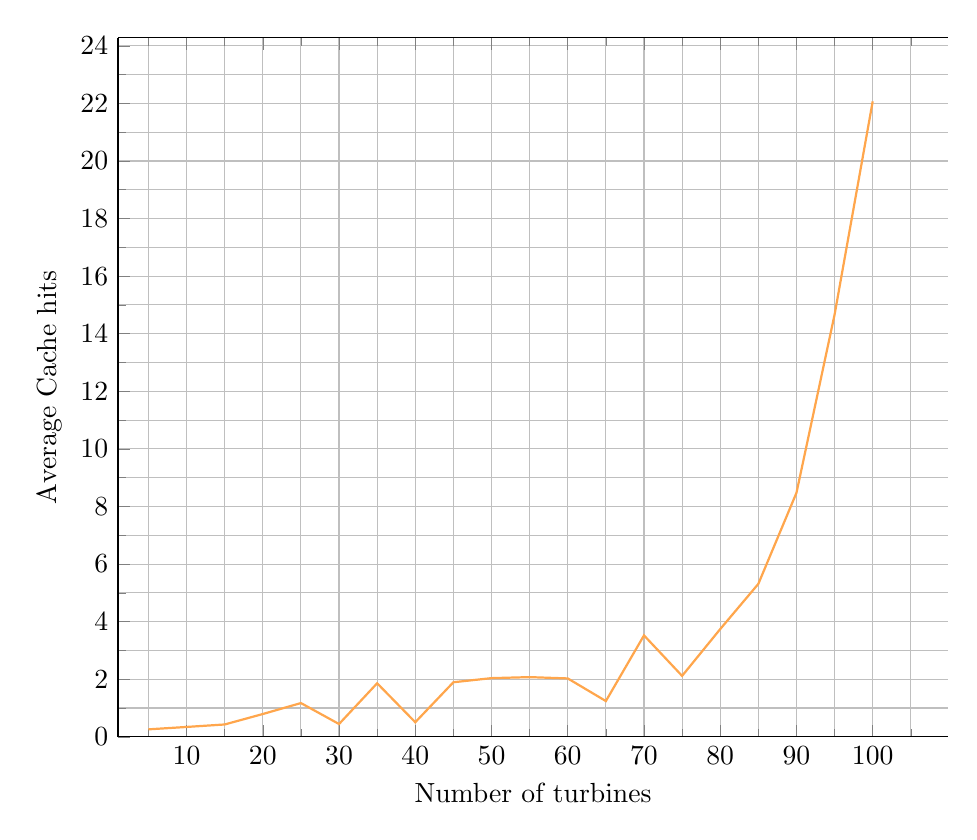
\begin{tikzpicture}
\begin{axis}
[
width=\resultsFigureWidthScale\textwidth,
axis y line*=left,
xlabel=Number of turbines,
ymin = 0,
xmin = 1,
ylabel=Average Cache hits,
%xtick={1, 2, 3, 4, 5, 6, 7, 8, 9, 10, 11, 12, 13, 14, 15, 16, 17, 18, 19, 20},
%xticklabels={5, 10, 15, 20, 25, 30, 35, 40, 45, 50, 55, 60, 65, 70, 75, 80, 85, 90, 95, 100},
%boxplot/draw direction=y,
grid=both,
minor tick num=1
]
%\buildBoxPlot[black]{0}{0}{0}{0}{0}
%\buildBoxPlot[black]{0}{0}{0}{0}{0}
%\buildBoxPlot[black]{0}{0}{0}{0}{0}
%\buildBoxPlot[black]{0}{0}{0}{0}{0}
%\buildBoxPlot[black]{0}{0}{0}{0}{0}
%\buildBoxPlot[black]{0}{0}{0}{0}{0}
%\buildBoxPlot[black]{0}{0}{0}{0}{0}
%\buildBoxPlot[black]{0}{0}{0}{0}{0}
%\buildBoxPlot[black]{0}{0}{0}{0}{0}
%\buildBoxPlot[black]{0}{0}{0}{0}{0}
%\buildBoxPlot[black]{0}{0}{0}{0}{0}
%\buildBoxPlot[black]{0}{0}{0}{0}{0}
%\buildBoxPlot[black]{0}{0}{0}{0}{0}
%\buildBoxPlot[black]{0}{0}{0}{0}{0}
%\buildBoxPlot[black]{0}{0}{0}{0}{0}
%\buildBoxPlot[black]{0}{0}{0}{0}{0}
%\buildBoxPlot[black]{0}{0}{0}{0}{0}
%\buildBoxPlot[black]{0}{0}{0}{0}{0}
%\buildBoxPlot[black]{0}{0}{0}{0}{0}
%\buildBoxPlot[black]{0}{0}{0}{0}{0}
\addplot[thick, orange!70] coordinates {
	(5 ,0.2591015249347438)
	(10 ,0.3423283799799435)
	(15 ,0.4286200856364344)
	(20 ,0.7913519050319182)
	(25 ,1.171919068056407)
	(30 ,0.4440826120490188)
	(35 ,1.8595523144717856)
	(40 ,0.506366007056297)
	(45 ,1.8951768000539848)
	(50 ,2.037951753081981)
	(55 ,2.0728170589196186)
	(60 ,2.0275369832294468)
	(65 ,1.2416290071090674)
	(70 ,3.5220372523313626)
	(75 ,2.115832267020478)
	(80 ,3.7417427229878832)
	(85 ,5.311682134712245)
	(90 ,8.473847137142263)
	(95 ,14.663734246038112)
	(100 ,22.06932793366117)
};
\end{axis}
\end{tikzpicture}
	\caption{Decentralized solution variable number of turbines experiment}
	\label{fig:exp:decen:turbines_cache}
\end{figure}


\Cref{fig:exp:decen:turbines_cache} shows the change in average cache reads when the number of turbines increase. The number of cache reads are below 4 from 5 turbines to 80 turbines, with an increasing trend. From 85 turbines to 95 turbines the number of cache reads increase with an exponential tendency. This can again be explained by limitations in the test setup, and the results should be disregarded.
        
        
\subsection{Discussion} 
The decentralized solution aims to detach the regulation cycle time from the number of turbines, by making reception of turbine state happen in parallel with the regulation cycle. As a consequence of this the term cache reads has been introduced to the system, since the detaching of receiving states from the regulation cycle opens for the possibility, that a given state from a turbine is used multiple times in a row for regulation. 

Looking at Experiment 1, we disregard the 10 ms data sets for both \cref{subsec:Exper:perfom:1} and \cref{fig:exp:decen:sleep-cache}, due to limited experiment equipment. Running with a 10 ms sleep time, caused our experiment setup to approach maximum network adapter capacity, due to too many packages, thus resulting in package delays.

Looking at \cref{subsec:Exper:perfom:1} we observe a linearly dependency between the sleep time and the regulation cycle time (with the 10 ms data set disregarded). This is expected since the sleep operation is a part of the regulation cycle. The outliers with lower values than the median, means we observe a lower regulation cycle time than the sleep time. This happens if the decentralized solution receives a new state from all turbines during the sleep operation, thus making the oldest state .



The outliers below the median are another matter. The reception of turbine states is decoupled from the regulation cycle meaning that whenever a turbine has a new state it will distribute it immediately. With the states of all turbines available at each turbine there is no need to wait for state updates before running the regulation algorithm. Regulation cycle time is calculated from the timestamp of reception of the oldest state used in the regulation algorithm to the timestamp taken just after the newly calculated state has been distributed. Thus, if all turbines have updated their state half way into the sleep time of the regulation cycle the time from the oldest received state until a new state is distributed may be smaller than the sleep time of the regulation cycle, embodied by the outliers that have a smaller regulation cycle time than the median.



Looking at \cref{fig:exp:decen:turbines} we see that the decentralized solution seems to be independent from the number of turbines, if the number of turbines is sufficiently low.
From 5 to 80 turbines the regulation cycle time is nearly constant at 20 ms.
The near constant regulation cycle time is caused by the fact that the regulation cycle in the decentralized solution is not forced to wait for data, before running the regulation algorithm because data is continually received in parallel with the regulation cycle. Adding a turbine to the decentralized solution adds an extra turbine state to read into the setpoint calculation in the regulation algorithm, thus adding network traffic to the system. 

When looking at regulation cycle time of the decentralized solution we must also look at the number of cache reads.
As explained in \cref{sec:exp:performance} a cache read happens when a turbine does not provide a new turbine state package before the next regulation cycle is started.
This forces the regulation cycle to use old turbine states from cache.
Looking at \cref{fig:exp:decen:turbines_cache} we see that the average number of cache reads in the decentralized solution are below 4 and increasing slightly until we reach 80 turbines. From there the number of cache reads increase exponentially.

The increase in regulation cycle time and cache reads when the number of turbines reaches 85 can be explained by the fact equipment used for this experiment is approaching maximum CPU capacity, which results in package delays. We use one computer for logging and two computers for simulating turbines, thus, when simulating 80 turbines, 40 turbines are run on the same computer.
Since regulation cycle time in the decentralized system is dependent on the reception time of the oldest turbine state package, the delayed packages has a direct impact on regulation cycle time.
Thus similarly lost or delayed network packages increases the use of cached data. The increased regulation cycle time and cache reads are thus not a limitation of the decentralized solution but a limitation imposed by the test setup. In order to create a realistic comparison we must disregard the results that are a direct effect of the limitations of our test setup.

Disregarding the limitations imposed by the test setup observe that the regulation cycle time is constant to the limit of turbines we can simulate. 

As stated above there is a small increase in regulation cycle time for every turbine added because the state of this turbine has to be taken into consideration when calculating new setpoints on all other turbines. This time addition is not visible in \cref{fig:exp:decen:turbines}. Thus the regulation cycle time will be affected by the addition of turbines but the effect is so small that it is indistinguishable by other factors.
The amount of outliers in \cref{fig:exp:decen:turbines} is fairly high. This is to be expected as the regulation cycle time factors in network traffic. Thus, the outliers that is higher than the median can be explained by a delay or a loss of a package in the network. Another explanation could be that the turbines are not running synchronized with each other. This means that one turbine may receive states from other turbines just at the time when the sleep time of the regulation cycle time elapses. Thus, it is possible that some turbines may not deliver their states in time for them to be used in the current regulation cycle which forces the use of cache reads, which in turn increases the regulation cycle time.


Still disregarding the limitations imposed by the test setup when looking at the number of cache reads we see another result. The number of cache reads increases slowly with a factor of around 1 cache read for every 30 turbines added, which gives a scale factor of $1 / 30 = 0.033$ added cache reads per turbine added.

The number of cache reads can be reduced by increasing the regulation cycle time as presented in \cref{fig:exp:decen:sleep-cache}.
Thus, the factor deciding the time of the regulation cycle is the maximum number of average cache reads accepted for a single regulation cycle.

\clearpage